%% This template can be used to write a paper for
%% Computer Physics Communications using LaTeX.
%% For authors who want to write a computer program description,
%% an example Program Summary is included that only has to be
%% completed and which will give the correct layout in the
%% preprint and the journal.
%% The `elsarticle' style is used and more information on this style
%% can be found at 
%% http://www.elsevier.com/wps/find/authorsview.authors/elsarticle.
%%
%%
%\documentclass[preprint,12pt]{elsarticle}

%% Use the option review to obtain double line spacing
%% \documentclass[preprint,review,12pt]{elsarticle}

%% Use the options 1p,twocolumn; 3p; 3p,twocolumn; 5p; or 5p,twocolumn
%% for a journal layout:
%% \documentclass[final,1p,times]{elsarticle}
%% \documentclass[final,1p,times,twocolumn]{elsarticle}
%% \documentclass[final,3p,times]{elsarticle}
%% \documentclass[final,3p,times,twocolumn]{elsarticle}
%% \documentclass[final,5p,times]{elsarticle}
%% \documentclass[final,5p,times,twocolumn]{elsarticle}

%% if you use PostScript figures in your article
%% use the graphics package for simple commands
%% \usepackage{graphics}
%% or use the graphicx package for more complicated commands
%\usepackage{graphicx}
%% or use the epsfig package if you prefer to use the old commands
%% \usepackage{epsfig}

%% The amssymb package provides various useful mathematical symbols
%\usepackage{amssymb}
%% The amsthm package provides extended theorem environments
%% \usepackage{amsthm}

%% Additional needed packages.
%\usepackage{amsmath}
%\usepackage{verbatim}
%\usepackage{color}

%% The lineno packages adds line numbers. Start line numbering with
%% \begin{linenumbers}, end it with \end{linenumbers}. Or switch it on
%% for the whole article with \linenumbers after \end{frontmatter}.
%\usepackage{lineno}
%\usepackage{hyperref}

%% natbib.sty is loaded by default. However, natbib options can be
%% provided with \biboptions{...} command. Following options are
%% valid:

%%   round  -  round parentheses are used (default)
%%   square -  square brackets are used   [option]
%%   curly  -  curly braces are used      {option}
%%   angle  -  angle brackets are used    <option>
%%   semicolon  -  multiple citations separated by semi-colon
%%   colon  - same as semicolon, an earlier confusion
%%   comma  -  separated by comma
%%   numbers-  selects numerical citations
%%   super  -  numerical citations as superscripts
%%   sort   -  sorts multiple citations according to order in ref. list
%%   sort&compress   -  like sort, but also compresses numerical citations
%%   compress - compresses without sorting
%%
%% \biboptions{comma,round}

% \biboptions{}

%% This list environment is used for the references in the
%% Program Summary
%%
%\newcounter{bla}
%\newenvironment{refnummer}{%
%\list{[\arabic{bla}]}%
%{\usecounter{bla}%
% \setlength{\itemindent}{0pt}%
% \setlength{\topsep}{0pt}%
% \setlength{\itemsep}{0pt}%
% \setlength{\labelsep}{2pt}%
% \setlength{\listparindent}{0pt}%
% \settowidth{\labelwidth}{[9]}%
% \setlength{\leftmargin}{\labelwidth}%
% \addtolength{\leftmargin}{\labelsep}%
% \setlength{\rightmargin}{0pt}}}
% {\endlist}

%\journal{Computer Physics Communications}

% ****** Start of file aipsamp.tex ******
%
%   This file is part of the AIP files in the AIP distribution for REVTeX 4.
%   Version 4.1 of REVTeX, October 2009
%
%   Copyright (c) 2009 American Institute of Physics.
%
%   See the AIP README file for restrictions and more information.
%
% TeX'ing this file requires that you have AMS-LaTeX 2.0 installed
% as well as the rest of the prerequisites for REVTeX 4.1
%
% It also requires running BibTeX. The commands are as follows:
%
%  1)  latex  aipsamp
%  2)  bibtex aipsamp
%  3)  latex  aipsamp
%  4)  latex  aipsamp
%
% Use this file as a source of example code for your aip document.
% Use the file aiptemplate.tex as a template for your document.
%\documentclass[%
% aip,
%%jmp,%
%%bmf,%
% sd,%
%%rsi,%
% amsmath,amssymb,
%%preprint,%
% reprint,%
%%author-year,%
%%author-numerical,%
%]{revtex4-1}

% Use this file as a source of example code for your aip document.
% Use the file aiptemplate.tex as a template for your document.
\documentclass[
 aps,
 jmp,
 amsmath,amssymb,
 twocolumn,
% preprint,%
% reprint,%
%author-year,%
%author-numerical,%
]{revtex4-1}

\usepackage{graphicx}% Include figure files
\usepackage{dcolumn}% Align table columns on decimal point
\usepackage{bm}% bold math
%\usepackage[mathlines]{lineno}% Enable numbering of text and display math
%\linenumbers\relax % Commence numbering lines
\usepackage{verbatim}
%\usepackage{subfloat}
%\usepackage{subcaption}
%\usepackage{placeins}
%\usepackage{caption}
%\captionsetup{font=scriptsize}
\usepackage{color}

%\usepackage{lineno}
\usepackage{hyperref}
% use st command to strike out text
\usepackage{soul}
\usepackage[makeroom]{cancel}

\newcommand{\pdv}[2]{\frac{\partial{#1}}{\partial{#2}}}
\newcommand{\fp}[2]{\pdv{#1}{#2}}
\newcommand{\pdwc}[3]{\left(\fp{#1}{#2}\right)_{#3}}
%\newcommand{\ppdv}[3]{\displaystyle \frac{\partial^2 #1}{\partial #2\partial #3}}
\newcommand{\ppdv}[3]{\frac{\partial^2 #1}{\partial #2\partial #3}}
\newcommand{\oover}[1]{\ensuremath{\frac{1}{#1}}}

\newcommand{\vect}[1]{\boldsymbol{#1}}
\newcommand{\matr}[1]{\mathbf{#1}}
\newcommand{\dI}{\text{d}}
\newcommand{\odv}[2]{\frac{\dI #1}{\dI #2}}
\newcommand{\ddv}[2]{\odv{#1}{#2}}
\newcommand{\christ}[3]{\genfrac{\{}{\}}{0pt}{}{#1}{#2 #3}}
%\newcommand{\christ}[3]{\Gamma^{#1}_{#2 #3}}
%\newcommand{\ddv}[2]{\frac{\Delta #1}{\Delta #2}}
\newcommand{\collpdv}[2]{\pdv{#1}{#2}\Big|_{coll}}
\newcommand{\mfp}{\lambda}
\newcommand{\tmfp}{\tilde{\lambda}}
\newcommand{\mfpe}{\lambda_e}
\newcommand{\mfpei}{\lambda_{ei}}
\newcommand{\Zbar}{\bar{Z}}
\newcommand{\nue}{\nu_{e}}
\newcommand{\nuei}{\nu_{ei}}
\newcommand{\nutot}{\nu_{t}}
\newcommand{\vmag}{v}
\newcommand{\vth}{v_{th}}
\newcommand{\vn}{\vect{n}}
\newcommand{\E}{\vect{E}}
\newcommand{\B}{\vect{B}}
\newcommand{\tE}{\vect{\tilde{E}}}
\newcommand{\tEz}{\tilde{E}_z}
\newcommand{\tB}{\vect{\tilde{B}}}
\newcommand{\qe}{q_e}
\newcommand{\me}{m_e}
\newcommand{\kB}{k_B}
\newcommand{\crs}{\sigma}
\newcommand{\fM}{f_M}
\newcommand{\tfM}{\tilde{f}_M}
\newcommand{\tvfM}{\vect{\tilde{f}_M}}
\newcommand{\daf}{\delta f}
\newcommand{\fzero}{f_0}
\newcommand{\dafzero}{\delta f_0}
\newcommand{\vfzero}{\vect{f_0}}
\newcommand{\davfzero}{\vect{\delta f_0}}
\newcommand{\fone}{\vect{f_1}}
\newcommand{\fonez}{f_{1_z}}
\newcommand{\SM}{\vect{S}_M}
\newcommand{\MI}{\matr{I}}
\newcommand{\MA}{\matr{A}}
\newcommand{\intO}{\int_{\Omega}}
\newcommand{\intv}{\int_{\vmag}}
\newcommand{\IM}{\boldsymbol{\mathcal{M}}}
\newcommand{\ID}{\boldsymbol{\mathcal{D}}}
\newcommand{\IV}{\boldsymbol{\mathcal{V}}}
\newcommand{\IB}{\boldsymbol{\mathcal{B}}}
\newcommand{\anisomega}{\fone/\fzero}
\newcommand{\acl}{\vect{M}_{\left(\anisomega\right)}}

\newcommand{\Wzero}{\psi}
\newcommand{\Wone}{\matr{w}}
\newcommand{\Wcurl}{\vect{W_c}}
\newcommand{\Wdiv}{\vect{W_d}}



\newcommand{\figref}[1]{FIG.~\ref{#1}}
\newcommand{\refeq}[1]{\eqref{#1}}
\newcommand{\secref}[1]{Section~\ref{#1}}
\newcommand{\appref}[1]{Appendix~\ref{#1}}
\newcommand{\tabref}[1]{TABLE~\ref{#1}}
\newcommand{\figscale}{0.48}


\begin{document}

\preprint{AIP/123-QED}

\title[AWBS kinetic modeling of electrons with nonlocal Ohm's law in plasmas relevant to inertial confinement fusion]{AWBS kinetic modeling of electrons with nonlocal Ohm's law in plasmas relevant to inertial confinement fusion}% Force line breaks with \\
%\thanks{Footnote to title of article.}

%\author{Authors}
\author{M. Holec}
 \email{holec1@llnl.gov}
 \affiliation{
Center for Applied Scientific Computing, Lawrence Livermore National
Laboratory, P.O. Box 808, L-561, Livermore, CA 94551, USA.
 }
 \affiliation{
Centre Lasers Intenses et Applications, Universite de Bordeaux-CNRS-CEA,\\ 
UMR 5107, F-33405 Talence, France.
}

\author{P. Loiseau}
 \affiliation{
 CEA, DAM, DIF, F-91297 Arpajon Cedex, France.
}

\author{J. P. Brodrick}
 \affiliation{
York Plasma Institute, Department of Physics, University of York,\\ 
Heslington, York, YO10 5DD, UK.
}

\author{D. Del Sorbo}
 \affiliation{
York Plasma Institute, Department of Physics, University of York,\\ 
Heslington, York, YO10 5DD, UK.
}

\author{A. Debayle}
 \affiliation{
 CEA, DAM, DIF, F-91297 Arpajon Cedex, France.
}

\author{V. Tikhonchuk}
 \affiliation{
Centre Lasers Intenses et Applications, Universite de Bordeaux-CNRS-CEA,\\ 
UMR 5107, F-33405 Talence, France.
}

\author{J.-L. Feugeas}
 \affiliation{
Centre Lasers Intenses et Applications, Universite de Bordeaux-CNRS-CEA,\\ 
UMR 5107, F-33405 Talence, France.
}

\author{Ph. Nicolai}
 \affiliation{
Centre Lasers Intenses et Applications, Universite de Bordeaux-CNRS-CEA,\\ 
UMR 5107, F-33405 Talence, France.
}

\author{B. Dubroca}
 \affiliation{
, Universite de Bordeaux,\\ 
France.
}

\author{C. P. Ridgers}
 \affiliation{
York Plasma Institute, Department of Physics, University of York,\\ 
Heslington, York, YO10 5DD, UK.
}

\author{R. J. Kingham}
 \affiliation{
Plasma Physics Group, Blackett Laboratory, Imperial College,\\ 
London SW7 2BW, United Kingdom.
}

\date{\today}% It is always \today, today,
             %  but any date may be explicitly specified

\begin{abstract}
\textit{A preliminary version...}
The~interaction of lasers with plasmas very often leads to nonlocal transport 
conditions, where the classical hydrodynamic model fails to describe 
physical phenomena, such as heat-flow, related to highly mobile particles. In this study 
the~electron distribution in plasma is investigated for the~conditions relevant 
to ICF. In particular, we focus on the~transport of nonlocal (supra-thermal) 
electrons streaming down the~temperature gradient in the~ablating plasma. 
Nevertheless, the~nature of plasma (ionized gas) requires a~correct response 
of background electrons too. This is achieved by the~action of an~electric 
field, which provides a~self-consistent Ohm’s law based on the~kinetic modeling.Our approach leans on the~Albritton-Williams-Bernstein-Swartz collision 
operator \cite{AWBS_PRL1986} providing a~simple, computationally efficient, 
transport equation of electrons and is further benchmarked against 
Vlasov-Fokker-Planck and collisional PIC codes. %CPR comment - could benefit from a clearer description of what the main results are, preferably with numbers
\end{abstract}

\pacs{Valid PACS appear here}% PACS, the Physics and Astronomy
                             % Classification Scheme.

\keywords{kinetics; nonlocal electron transport; laser-heated plasmas; hydrodynamics, Ohm's law.}%Use showkeys class option if keyword display desired

\maketitle


%%
%% Start line numbering here if you want
%%
% \linenumbers

%\pagebreak
%\tableofcontents
%\pagebreak
%% main text
%\section{}
%\label{}
%---------------------------------------------------------------------
%---------------------------------------------------------------------

\section{Introduction}
\label{sec:Intro}
%In dealing with the nonequilibrium properties of
%systems whose particles obey an inverse-square law
%of interaction, it is convenient to make use of the fact
%that under most circumstances small-angle collisions
%are much more important than collisions resulting in
%large momentum changes. This leads to the method
%often used for treating such systems, in which one
%expands the collision integrand of the Boltzmann change per
%equation in powers of the momentum collision.

The~first modern attempts at kinetic modeling of plasma can be traced back 
to the~fifties, when Cohen, Spitzer, and Routly (CSR) \cite{CSR_1950} 
demonstrated that the~effect of Coulomb collisions between electrons and ions 
in the~ionized gas predominantly results 
from frequently occurring events of cumulative small deflections 
rather than occasional close encounters. This effect was originally described
by Jeans in \cite{Jeans_BOOK1929} and 
Chandrasekhar \cite{Chandrasekhar_RMP1943} 
proposed to use the~diffusion equation model of the~Vlasov-Fokker-Planck type 
(VFP)~\cite{Planck_1917}.
%CPR comment - do you need to start so far back in the history of plasma kinetic theory?


%A more generally valid approach to the problem of
%treating changes in a distribution function resulting
%each of which from frequently occurring "events",
%produces a small change in the momentum of a particle,
%is to use the Fokker-Planck equation \cite{Planck_1917}, 
%which has been discussed by Spitzer and collaborators 
%\cite{SpitzerHarm_PR1953} . 
A~classical paper by Spitzer and H\"arm (SH) 
\cite{SpitzerHarm_PR1953} provides the~computation of 
the~electron distribution function (EDF) in a~plasma (from low to high $\Zbar$)
with a~temperature gradient accounting for electron-electron (e-e) and 
electron-ion (e-i) collisions.
The~resulting expressions for current and heat flux are widely used in plasma 
hydrodynamic models.
%used the formalism of the VFP equation to evaluate the collision terms of 
%the~Boltzmann equation under the assumptions that 
%(a) the events producing changes in particle momenta
%are two-body interactions described by the associated
%differential scattering cross sections, and 
%(b) that 
The~distribution function based on the spherical harmonics method in 
its first approximation (P1) \cite{Jeans_MNRAS1917} is of the form 
$f^0+\mu f^1$, where $f^0$ and $f^1$ 
are isotropic and $\mu$, is the direction cosine between the particle 
velocity and the~temperature gradient. It should be emphasized that
the~SH solution assumes a~small perturbation from equilibrium, i.e. that 
$f^0$ is the~Maxwell-Boltzmann distribution and $\mu f^1$ represents 
a~very small anisotropic deviation. 
This approximation holds for $L_T\gg\mfpe$, 
a~condition which is often invalid in laser plasmas, 
where $L_T$ is the~temperature length scale and $\mfpe$ 
the~mean free path of electrons. Note that electrons having
3 to 4 times the~thermal velocity are dominantly responsible for heat-flow
and that those faster than 6 times the~thermal velocity can be completely 
neglected in this local theory.

%It is the purpose of this paper to present the mechanics 
%of two-body collisions in a somewhat simplified
%form, and to derive the Fokker-Planck equation for an function. 
%From this general arbitrary distribution equation such special cases 
%as those of Chandrasekhar and Spitzer may easily be obtained. 
%For more complex situations the equation is suitable for integration by an
%electronic computer \cite{Rosenbluth_PR1957}.

The~actual cornerstone of the~modern VFP simulations was set in place
by Rosenbluth \cite{Rosenbluth_PR1957}, when he derived a~simplified form 
of the~VFP equation for a~finite expansion of the~distribution function,
where all the~terms are computed according to plasma conditions, including
$f^0$, which of course needs to tend to the~Maxwell-Boltzmann distribution.
% CPR comment - again not sure you need to go back this far in history.
Consequently, the~pioneering work on numerical solution of the~VFP equation
\cite{Bell_1981_83, Matte_1982_86} revealed the~importance of the~nonlocal
electron transport in laser-heated plasmas. 
In particular, that the~heat flow down steep temperature gradients in 
unmagnetised plasma cannot be described by the classical, local fluid
description of transport \cite{SpitzerHarm_PR1953, Braginskii_1965_3}.
This is due to the~classical $f^1$ \textit{not being} a~small deviation 
(especially for electrons having 3 to 4 times the~thermal velocity), 
i.e. $f^0\sim f^1$ characterized by $L_T\sim\mfpe$.
It was also shown that a~thermal transport inhibition \cite{Bell_1981_83} 
around the peak of the temperature gradient, and a~nonlocal preheat 
ahead of the main heat wave front, naturally appear. 
These effects are attributed to significant deviations 
of $f^0$ from Maxwellian distribution.


%Previously the Vlasov-Fokker-Planck (VFP) equation has been solved
%numerically ignoring magnetic fields in 1-D (1 spatial dimension) 
%\cite{Bell_1981_83, Matte_1982_86} to address heatflow down steep temperature 
%gradients in unmagnetised plasma. Under these conditions the classical, fluid
%description of transport \cite{SpitzerHarm_PR1953, Braginskii_1965_3}, 
%which makes the local approximation, 
%breaks down. They found that nonlocal effects are responsible for 
%thermal transport inhibition \cite{Bell_1981_83}.

%Particle-in-cell (PIC) codes \cite{PIC_Birdsall_Langdon_1985}
%%\cite{Dawson_PoF1962, PIC_Birdsall_Langdon_1985} 
%%and Vlasov codes $[23]$ 
%are fully kinetic and are ideally suited to collisionless plasmas. 
%Typically PIC codes tend to use explicit methods and consequently require a
%time step small enough to resolve the fastest frequency present in the problem.
%They also suffer from the so called "finite grid instability" 
%\cite{PIC_Birdsall_Langdon_1985} 
%whereby the plasma numerically heats up until the electron debye length is
%resolved by the grid. These limitations mean that multidimensional, explicit, 
%PIC cannot readily simulate the low temperature, high density plasma 
%created inlaser–solid interactions. 
%%PIC codes utilising implicit methods do exist 
%%$[24]$. Implicitness greatly relaxes the time step constraint and mitigates 
%%the effects of the finite grid instability, so that lower temperatures 
%%and higher densities can be dealt with. 
%One spatial dimension PIC codes with electron–ion collisions have successfully 
%been applied to fast electron transport through solid density plasma 
%\cite{Guerin_PPCF1999, Perez_PoP2012}. 
%%Two spatial dimension PIC codes with electron collisions also exist, both
%%explicit $[25]$ and implicit $[26]$. 

%Explicit 2-D PIC is unable to access conditions where collisions dominate for
%the bulk of the electrons, though. Even though implicit methods overcome 
%this particular problem, the PIC method in general struggles to adequately 
%resolve the distribution function in a given cell when a realistic sized, 
%2-D problem is addressed. 
%Statistical noise and under resolution of 
%the electron distribution lead to an inaccurate treatment of collisions and 
%can overwhelm real physical effects present.

Nevertheless, numerical solution of the~VFP equation even in the~Rosenbluth
formalism remains very challenging computationally, because the~e-e collision
opereator is nonlinear due to its intrego-differential nature. 
More simple linear forms of e-e collision operator
are needed. Although some VFP simulations on experimentally relevant timescales 
have been performed (for recent examples see 
\cite{Hawreliak04,Ridgers08,Willingale10,Bissell10,Joglekar14,Joglekar16,Henchen_PRL2018}, 
an extensive review has been conducted by Thomas et al. \cite{Thomas13}), 
their relative computational inefficiency severely limits the range of 
simulations that can be performed.

The~purpose of this paper is to use an~efficient alternative 
to a full solution of the VFP equation introduced in \cite{Sorbo_2015}
to accurately calculate nonlocal transport, 
based on the~Albritton-Williams-Bernstein-Swartz 
collision operator (AWBS) \cite{AWBS_PRL1986}.
In Section \ref{sec:AWBSmodel} we propose a~modified form of 
the~AWBS collision operator. The~important properties of this operator 
are further presented in Section \ref{sec:DiffusiveKinetics} 
with the~emphasis on its
comparison to the~full VFP solution in the~local diffusive regime.
In \secref{sec:AWBSnonlocal} we define a~full model of electron kinetics and 
the~way of discretizing the~electron phase-space and also
the~coupling of the~kinetic model to magneto-hydrodynamics.
Section \ref{sec:BenchmarkingAWBS} focuses on the~performance of the~AWBS 
transport equation model compared to modern kinetic codes including VFP codes
Aladin and Impact \cite{Kingham_JCP2004}, and PIC code Calder 
\cite{Perez_PoP2012}, where the~cases related to real
laser-generated plasma conditions are studied. Finally, the~most important
outcomes of our research are concluded in Section \ref{sec:Conclusions}. 

\section{The~AWBS kinetic model}
\label{sec:AWBSmodel}

The~electrons in plasma can be modeled by the~deterministic Vlasov model 
of charged particles
\begin{equation}
  \pdv{\ft}{t} + \vv\cdot\gx \ft + 
  \frac{\qe}{\me}\left(\E + \frac{\vv}{c}\vect{\times}\B\right)\cdot\gv \ft = 
  C_{ee}(f) + C_{ei}(f) ,
  \label{eq:kinetic_equation}
\end{equation}
where $\ft(t, \vect{x}, \vect{v})$ represents the~density function of electrons
at time $t$, spatial point $\vect{x}$, and velocity $\vv$, $\E$ and $\B$ are 
the~electric and magnetic fields in plasma, $\qe$ and $\me$ being 
the~charge and mass of electron.

The~general form of the~e-e collision operator 
$C_{ee}$ is the~Fokker-Planck form published by Landau \cite{Landau_1936}
\begin{equation}
  C_{FP}(\ft) =
  \Gamma\int \gv\gv(\vv - \vvb) \cdot \left(
  \ft\, \gvb \ft - \ft\, \gv \ft \right)\, \dI\vvb ,
  \label{eq:LFP_model}
\end{equation}
where $\Gamma = \frac{4\pi\qe^4\lnc}{\me^2}$ and 
$\lnc$ is the~Coulomb logarithm.
The~e-i collision operator $C_{ei}$ could be expressed
in a~simpler form since massive ions are considered 
to be motionless compared to electrons \corrCPR{during a collision}. %CPR comment - sorry for the pedantic distinction just clarifying that it is possible to account for ion motion in the VFP equation while ignoring it in the collision operator
 The~scattering operator accounts
for the~change of electron velocity without change in the~velocity magnitude\corrCPR{, i.e. angular scattering}. 
It is expressed in spherical coordinates as
\begin{equation}
  C_{ei}(\ft) = \frac{\nuei}{2}
  \left(\pdv{}{\mu}\left((1 - \mu^2)\pdv{\ft}{\mu}\right)
  + \frac{1}{\sin^2\phi}\frac{\partial^2 \ft}{\partial\theta^2} \right) ,
  \label{eq:ei_scattering}
\end{equation}
where $\mu = \cos\phi$, $\phi$ and $\theta$ are the~polar and azimuthal 
angles, and $\nuei = \frac{\Zbar n_e \Gamma}{\vmag^3}$ is the~e-i
collision frequency.

The~e-e collision operator needs to be linearized for efficient computation\corrCPR{\st{s}}.
Fis\corrCPR{c}h introduced a~linear form of $C_{ee}$ in \cite{Fish_RMP1987} 
in the~high-velocity limit ($\vmag\gg\vth$) electron collision operator
\begin{multline}
  C_{H}(\ft) = \vmag \nue \pdv{}{\vmag}\left(\ft + 
  \frac{\vth^2}{\vmag}\pdv{f}{\vmag}\right) \\
  + \frac{\nue}{2}\left( 1 - \frac{\vth^2}{2\vmag^2}\right) 
  \left(\pdv{}{\mu}\left((1 - \mu^2)\pdv{f}{\mu}\right)
  + \frac{1}{\sin^2\phi}\frac{\partial^2f}{\partial\theta^2} \right)
  , \label{eq:HighVelocity_model}
\end{multline}
where $\nue = \frac{n_e \Gamma}{\vmag^3}$ is the~e-e collision 
frequency and $\vth = \sqrt{\frac{\kB T_e}{\me}}$ is the~electron thermal 
velocity.
The~linear form of $C_{H}$ arises from an~assumption that the~fast electrons 
predominantly interact with the~thermal (slow) electrons, 
which \corrCPR{ is an important simplification to} the~form \eqref{eq:LFP_model}.
However the~diffusion term in the~e-e collision operator 
\eqref{eq:HighVelocity_model} still presents numerical difficulties.

A~yet simpler form of the~collision operator of electrons was proposed in 
\cite{Sorbo_2015}
\begin{multline}
  C_{AWBS}(\ft) = \vmag \nue^*\pdv{}{\vmag}\left(\ft - \fM\right) \\
  + \frac{\nuei + \nue^*}{2} 
  \left(\pdv{}{\mu}\left((1 - \mu^2)\pdv{f}{\mu}\right)
  + \frac{1}{\sin^2\phi}\frac{\partial^2f}{\partial\theta^2} \right)
  , \label{eq:AWBS_model}
\end{multline}
where $\fM = \frac{n_e}{(2\pi)^{\frac{3}{2}}\vth^3}
\exp\left(-\frac{\vmag^2}{2\vth^2}\right)$ 
is the~Maxwell-Boltzmann equilibrium distribution.
Here, the~first term representing the AWBS operator \cite{AWBS_PRL1986}
accounts for relaxation to equilibrium due to the~e-e collisions, and 
the~second term accounts for the~e-i and e-e collisions contribution 
to scattering.

A~method of angular momenta for the~solution of the~electron kinetic equation
with the~collision operator \eqref{eq:AWBS_model} 
was introduced in \cite{Sorbo_2015, Sorbo_2016}. 

In \eqref{eq:AWBS_model} we have introduced a~modified e-e collision frequency
$\nue^*$ in order to address a~proper behavior with respect to $\Zbar$, which
is further analyzed in Section \ref{sec:DiffusiveKinetics} and promising 
results compared to the~full FP operator are presented.

%The~Maxwell-Boltzmann averaged e-e scattering in 
%\eqref{eq:HighVelocity_model} can be approximated as 
%$\nue \int\left(1 - \frac{\vth^2}{2\vmag^2}\right)\fM 4\pi\vmag^2\, \dI\vmag = 
%\frac{\nue}{2}$.

\section{BGK, AWBS, and Fokker-Planck models in local diffusive regime}
\label{sec:DiffusiveKinetics}

%In a~broad analysis of the~electron transport, any qualitative information
%about its properties are highly welcome. Even better, if one can extract some 
%qualitative information, which provides comparative and reliable results in 
%a~clear way, the~confidence of using a~transport model, 
%e.g. \eqref{eq:AWBS_model}, can lead to efficient yet relatively
%cheap computation cost predictions of real physics.

An~approximate solution to the~so-called \textit{local diffusive regime} 
of electron transport can be found, since the~\textit{diffusive regime}
refers to a~low anisotropy given by the~projection $\mu$. i.e.
modeled by the~P1 form of EDF  
\begin{equation}
  \tilde{\ft}(z, \vmag, \mu) = \ft^0(z, \vmag) + \mu \ft^1(z, \vmag),
  \label{eq:f_approximation}
\end{equation}
where $z$ is the~spatial coordinate along the~axis $z$, $\vmag$ 
the~magnitude of transport velocity. 
%and $\mu = \cos\phi$, where $\phi$ 
%is the~pitch angle with respect to the~axis $z$.

%In the~words of mathematics this corresponds to the~first 
%order expansion in $\mfpei$ and $\mu$ of the~distribution function as
%\begin{equation}
%  \tilde{\ft}(z, \vmag, \mu) = \ft^0(z, \vmag) + \ft^1(z, \vmag) \mfpei\mu ,
%  \label{eq:f_approximation}
%\end{equation}
%where $z$ is the~spatial coordinate along the~axis $z$, $\vmag$ the~magnitude 
%of transport velocity, and 
%$\mfpei = \frac{\vmag}{\nuei} = \frac{\vmag^4}{\Zbar n_e \Gamma}$.
%In other words, one can say that by evaluating numerically $\tilde{\ft}$
%in \eqref{eq:f_approximation}, we accept some error of the~order 
%$O(\mfpei^2) + O(\mu^2)$. The~expansion in a~small parameter $\mfpei$ is also
%coherent with a~time-steady approximation due to the~relation between the~mean
%free path and collision frequency, where the~higher the~collision frequency 
%the~more steady the~solution. 

The~approximate transport solution is then obtained when analyzing 
the~action of the~time-steady form of \eqref{eq:kinetic_equation} in 1D 
on the~approximation \eqref{eq:f_approximation} as
\begin{equation}
  \mu\left(\pdv{\tilde{f}}{z} 
  + \frac{\qe\Ez}{\me\vmag}\pdv{\tilde{f}}{\vmag}\right) 
  + \frac{\qe\Ez}{\me}\frac{(1-\mu^2)}{\vmag^2}\pdv{\tilde{f}}{\mu}
  %\mu\left(\pdv{f^0}{z} + \frac{\Ez}{\vmag}\pdv{f^0}{\vmag}\right) 
  %+ \frac{\Ez\mfpei}{\vmag^2} f^1 
  = \frac{1}{\vmag}C(\tilde{\ft}) ,
  \label{eq:1D_kinetic_equation}
\end{equation}
where $C$ is a~given collision operator including both e-e and e-i collisions.

The~locality of transport is the~best expressed in terms of the~Knudsen number
$Kn=\frac{\lambda}{L}$, where $\lambda$ is the~mean free path of electron and
$L$ the~characteristic length scale of plasma. Consequently, plasma conditions
characterized by $Kn\ll1$ exhibit a~local transport regime. This measure then
play a~very important role in our analysis, where we use the~electron-electron
and electron-ion mean free paths $\mfpe = \Zbar\mfpei = \frac{\vmag}{\nue}$,
and the~density and temperature plasma scale lengths 
$L_{n_e} = n_e/\pdv{n_e}{z}$ and $L_{T_e} = T_e/\pdv{T_e}{z}$.

In practice, the~Knudsen number of thermal electrons is often used as 
a~measure of the~locality of transport corresponding to given plasma conditions,
where $Kn(\vth)<0.001$ is considered the~limit of validity of 
the~local transport theory \cite{LMV_1983_7}.


\subsection{The~BGK local diffusive electron transport}
\label{sec:BGKDiffusiveRegime}

Bhatnagar, Gross, and Krook  introduced a~very simple form
of a~collision operator \cite{BGK_1954}
\begin{equation}
  C_{BGK}(\tilde{\ft})
  =
  \nue(\fM - \tilde{\ft})
  + \frac{\nuei + \nue}{2}
  \pdv{}{\mu}(1 - \mu^2)\pdv{\tilde{\ft}}{\mu} .
  \label{eq:BGK_model_1D}
\end{equation}
In spite of its~simple form, BGK collision operator \eqref{eq:BGK_model_1D} 
serves as a~useful model providing a~relevant kinetic response, yet only 
qualitative with respect to the~FP collision operator \eqref{eq:LFP_model}.
In particular, the~conservation of kinetic energy, momentum, 
and number of particles is often violated 
\cite{Shkarofsky_Particle_Kinetics_book_1966_24}.

%of the~Boltzmann transport collision 
%operator, because of two reasons: a) it can be treated analytically in 
%the~local diffusive regime; and b) it represents the~so-called phenomenological
%collision operator by explicitly using the~Maxwell-Boltzmann equilibrium 
%distribution $\fM$, which proves to be very useful in coupling of the~nonlocal 
%electron transport to hydrodynamics.

%If one applies the~action of the~right hand side, i.e. of 
%\eqref{eq:BGK_model_1D}, 
%on the~approximation \eqref{eq:f_approximation} and sets the~result to be equal 
%to the~left hand side \eqref{eq:LHS_kinetic_equation}, the~corresponding terms
%in $\mu$ are governed by the~following equations
However, the~form of \eqref{eq:BGK_model_1D} provides a~simple analytical 
treatment of local diffusive transport regime, when used in 
\eqref{eq:1D_kinetic_equation}. As a~result, one finds a~simple form of
the~BGK isotropic and anisotropic terms of \eqref{eq:f_approximation} to be
\begin{eqnarray}
  \ft^0 &=& \fM ,
  % \frac{\vth^2}{\vmag^2}f^1 ,
  \label{eq:BGK_f0} \\
  \ft^1 &=& - \frac{\mfpe}{\Zbar + 2}
  \left( \pdv{\fM}{z} + \frac{\qe\Ez}{\me\vmag}\pdv{\fM}{\vmag} \right) ,
  %\left( \pdv{\ft^0}{z} + \frac{\qe\Ez}{\me\vmag}\pdv{\ft^0}{\vmag} \right) , 
  \label{eq:BGK_f1}
\end{eqnarray}
where 
%$Kn = \frac{\mfpe}{L_{n_e}} + \frac{5}{2}\frac{\mfpe}{L_{T_e}}$
a~detailed derivation of \eqref{eq:BGK_f0} and \eqref{eq:BGK_f1} 
can be found in Appendix~\ref{app:DiffusiveKinetics}.
When the~quasi-neutrality constraint imposed by $\E_L$
\eqref{app_eq:BGK_Efield} is used, one finally obtains the~analytical BGK form 
of the~anisotropic term %\eqref{eq:f_approximation}
\begin{equation}
  \ft^1 = - \mu 
  \left( \frac{\vmag^2}{2 \vth^2} - 4\right)\frac{1}{\Zbar + 2}
  \frac{\mfpe}{L_{T_e}}\fM
  %\tilde{\ft}_{BGK} = \fM - \mu 
  %\left( \frac{\vmag^2}{2 \vth^2} - 4\right)\frac{1}{\Zbar + 2}
  %\frac{\mfpe}{L_{T_e}}\fM 
  . 
  \label{eq:BGK_approximation}
\end{equation}
The~details about the~BGK distribution function compared to other
collision operators can be found in Section~\ref{sec:SummaryDiffusiveKinetics}.

\subsection{The~AWBS local diffusive electron transport}
\label{sec:AWBSDiffusiveRegime}
%The~main object of this work presented in Sec~\ref{sec:AWBSmodel} simplifies
%in 1D to a~relatively simple form of the~Boltzmann transport collision operator
%(compared to \eqref{eq:LFP_model})
%\begin{equation}
%  C_{AWBS}(f)
%  = 
%  \vmag \nue^* \pdv{}{\vmag}\left(f - \fM\right) %\\
%  + \frac{\nuei + \nue^*}{2}\pdv{}{\mu}(1 - \mu^2)\pdv{f}{\mu} .
%  \label{eq:AWBS_model_1D}
%\end{equation}
Similarly to the~BGK model, the~AWBS collision operator \ref{eq:AWBS_model} 
explicitly uses equilibration to the~Maxwell-Boltzmann distribution $\fM$. 
On the~other hand, AWBS originates from $C_H$, which is derived from 
the~full FP operator \eqref{eq:LFP_model}. This makes the~AWBS operator 
to be superior to the~BGK operator, which is considered a~purely
phenomenological model.
%and also, 
%makes it a~very attractive model of the~nonlocal electron
%transport to be coupled to hydrodynamics via the~plasma electron temperature 
%and density.

%A~qualitative information about the~AWBS model is obtained while repeating
%the~action on \eqref{eq:f_approximation} by the~left hand side 
%\eqref{eq:LHS_kinetic_equation} and by the~right hand side 
%\eqref{eq:AWBS_model_1D} and setting the~equality. The~corresponding terms
%in $\mu$ are then governed by the~following equations
If \eqref{eq:AWBS_model} is used in \eqref{eq:1D_kinetic_equation}, one obtains
the~following equations governing the~AWBS isotropic and anisotropic terms of 
\eqref{eq:f_approximation}
\begin{eqnarray}
  \pdv{f^0}{\vmag} &=& \pdv{\fM}{\vmag} ,
  %+ Kn \frac{\vth^2}{\vmag^2}\frac{f^1}{\vmag} ,
  \label{eq:AWBS_f0} \\
  \pdv{f^1}{\vmag}  
  - \frac{\Zbar +  r_A}{\vmag r_A} f^1 &=& 
  %\frac{\mfpe}{\vmag\zeta}
  %\left(\pdv{f^0}{z} + \frac{\qe\Ez}{\me\vmag}\pdv{f^0}{\vmag}\right) ,
  \frac{\mfpe}{\vmag r_A}
  \left(\pdv{\fM}{z} + \frac{\qe\Ez}{\me\vmag}\pdv{\fM}{\vmag}\right) ,
  \label{eq:AWBS_f1} 
  %\\  
  %\frac{\vmag}{\Zbar}\pdv{f^1}{\vmag} + \frac{4}{\Zbar}f^1 
  %- \frac{\Zbar + 1}{\Zbar} f^1 &=&
  %\pdv{f^0}{z} + \frac{\tilde{E}_z}{\vmag}\pdv{f^0}{\vmag}
  %\nonumber
\end{eqnarray}
where $ r_A$ represents a~scaling parameter defining the~modified
e-e collision frequency as $\nue^* =  r_A \nue$.
A~detailed derivation of \eqref{eq:AWBS_f0} and \eqref{eq:AWBS_f1} 
can be found in Appendix~\ref{app:DiffusiveKinetics}.
%One observes that $\ft^0$ goes to Maxwellian when 
%the~local regime of transport is settled. 
%Indeed, according to equation~\eqref{eq:AWBS_f0} the~derivative 
%$\pdv{\ft^0}{\vmag}\rightarrow\pdv{\fM}{\vmag}$  when $Kn\ll1$ for any 
%electron velocity, thus leading to $\ft^0\rightarrow\fM$.
Consequently, one finds the~AWBS model equation for $\ft^1$ 
in local diffusive regime to be
%i.e. $\ft^0 = \fM + O(\mfpei^2)$, however, the~$\ft^1$ does not have 
%a~straightforward analytic formula. In reality, $\ft^1$ arises from 
%the~ordinary differential equation 
%(by inserting $\fM$ into \eqref{eq:AWBS_f1})
\begin{multline}
  \pdv{f^1_{\text{AWBS}}}{\vmag} 
  + \frac{\Zbar +  r_A}{\vmag r_A}f^1_{\text{AWBS}}
  = \\
  \frac{\mfpe}{\vmag r_A}\left(\frac{1}{L_{n_e}} + 
  \left( \frac{\vmag^2}{2 \vth^2} - \frac{3}{2}\right)
  \frac{1}{L_{T_e}} - \frac{\qe\Ez}{\me\vth^2}\right)\fM .
  %\frac{\mfpe}{\vmag}\left(\frac{1}{n_e}\pdv{n_e}{z} + 
  %\left( \frac{\vmag^2}{2 \vth^2} - \frac{3}{2}\right)
  %\frac{1}{T}\pdv{T}{z} - \frac{\qe\Ez}{\me\vth^2}\right)\fM .
  \label{eq:AWBS_f1_ODE}
\end{multline}
which can be solved analytically by using quadratures
\begin{equation}
  \text{Vladimir's analytical formula} .
  \label{eq:VT_quadratures}
\end{equation}
\begin{comment} % Substitute with Vladimir's analytical formula.
Since there is no simple analytical formula for $\ft^1$ solving 
\eqref{eq:AWBS_f1_ODE}, we adopt the~implicit Euler numerical integration
with $\Delta v < 0$, i.e. we integrate from high electron velocity 
($v_{max} = 7\vth$) to the~velocity equal to zero (using 10$^4$ steps). 
This mimics a~particle deceleration due to collisions. The~correct numerical
solution of \eqref{eq:AWBS_f1_ODE} corresponds to an~appropriate value of 
$\Ez$ leading to a~zero current. 
%Interestingly, this numerical value matches
%precisely the~Spitzer electric field \eqref{app_eq:BGK_Efield}.
As in the~BGK case, the~numerical solution of \eqref{eq:AWBS_f1_ODE} reveals
that $\ft^1 \sim Kn \fM$ and that $\ft^0$ equilibrates to $\fM$ 
as $O(Kn^2)$ based on \eqref{eq:AWBS_f0}.
\end{comment} % Substitute with Vladimir's analytical formula.

The~details about the~AWBS distribution function compared to other
collision operators and a~proper evaluation of the~scaling parameter $ r_A$
can be found in Section~\ref{sec:SummaryDiffusiveKinetics}.

\subsection{The~Fokker-Planck local diffusive electron transport}
\label{sec:FPDiffusiveRegime}

The~solution to the~1D transport equation \eqref{eq:1D_kinetic_equation}
using the~Fokker-Planck collision operator \eqref{eq:LFP_model}
is very ambitious, as demonstrated in 
\cite{Chandrasekhar_RMP1943, CSR_1950, Rosenbluth_PR1957}, fortunately, one 
can use the~explicit evaluation of the~electron distribution function
published in \cite{SpitzerHarm_PR1953}, which takes the~following form
\begin{multline}
  %\ft^1(\vmag, \mu) 
  \ft^1_{\text{SH}} = %\frac{\me^2}{4 \pi \qe^4\lnc} 
  \frac{\vtwoh^4}{\Gamma\Zbar n_e}\\
  \left( 2\tilde{D}_T\left(\frac{\vmag}{\vtwoh}\right) 
  + \frac{3}{2}\frac{\gamma_T}{\gamma_E} 
  \tilde{D}_E\left(\frac{\vmag}{\vtwoh}\right) \right)%\\ 
  \frac{\fM}{T}\pdv{T_e}{z}  ,
  \label{eq:f1_SH}
\end{multline}
where $\tilde{D}_T(x) = \Zbar D_{T}(x) / B$, 
$\tilde{D}_E(x) = \Zbar D_{E}(x) / A$, $\gamma_T$,
and $\gamma_E$ are numerical values in TABLE~I, TABLE~II, and
TABLE~III in \cite{SpitzerHarm_PR1953}, and 
$\vtwoh = \sqrt{\frac{\kB T_e}{2\me}}$.

One should be aware, that the~solution of \eqref{eq:1D_kinetic_equation}
equipped with the~full FP collision operator reveals the~importance of
e-e Coulomb collisions, which is emphasized in the~$\Zbar$ dependence 
of the~distribution function, current, heat flux, electric field, etc.
In particular, the latter exhibits the~following dependence 
\cite{SpitzerHarm_PR1953}
\begin{equation}
  \E = \frac{\me \vth^2}{\qe}
  \left(\frac{\nabla n_e}{n_e} + 
  \left(1 + \frac{3}{2}\frac{\Zbar + 0.477}{\Zbar + 2.15} \right)
  \frac{\nabla T_e}{T_e} \right),
  \label{eq:SH_Efield} 
\end{equation}
which for $\Zbar\gg1$ corresponds to the~classical Lorentz electric field 
\eqref{app_eq:BGK_Efield}.

%In the~case of high $\Zbar$ limit, $\gamma_T \rightarrow 1$,
%$\gamma_E \rightarrow 1$, $d_E(x) = x^4$, and $d_T(x) = x^4 (2.5 - x^2)/2$
%\cite{SpitzerHarm_PR1953}, which leads to the~standard Lorentz gas model
%\begin{equation}
%   f_1(\vmag, \theta) = \cos(\theta) \frac{\me^2}{4 \pi e^4\lnc} 
%  \frac{\vmag^4}{\Zbar}\left( 4 - \frac{\vmag^2}{\vtwoh^2} \right) 
%  \frac{\fM(\vmag)}{n_e}\frac{\nabla T}{T}  ,
%  \label{eq:f1_Lorentz} 
%\end{equation} 

\subsection{Summary of the~BGK, AWBS, and Fokker-Planck local diffusive 
transport}
\label{sec:SummaryDiffusiveKinetics}

Ever since the~SH paper \cite{SpitzerHarm_PR1953}, the~effect of microscopic
electron transport on the~current $\int \qe \vv \tilde{\ft} \, \dI\vv$ 
and the~heat flux $\int \frac{\me |\vv|^2}{2} \vv \tilde{\ft} \, \dI\vv$ 
in plasmas
under local diffusive conditions has been understood. By overcoming some 
delicate aspects of the~numerical solution to \eqref{eq:LFP_model} presented 
in the~CSR paper \cite{CSR_1950}, the~effect of electron-electron collisions
was properly quantified and the~correct dependence on $\Zbar$ of the~heat flux
$\vect{q}$ was approximated as \cite{SpitzerHarm_PR1953} 
\begin{equation}
  \vect{q} = \xi(\Zbar)~\vect{q}_L 
  = \frac{\Zbar + 0.24}{\Zbar + 4.2} \vect{q}_L ,
  \label{eq:qSH_approximation}
\end{equation}
where 
$\xi$ is the~$\Zbar$-dependence \cite{Epperlein_PoFB1991} approximation and
$\vect{q}_L$
%$\vect{q}_L = \kappa T_e^{\frac{5}{2}}\nabla T_e$ 
is the~heat flux given 
by the~Lorentz gas model \cite{Lorentz_1905} 
\begin{equation}
  \ft^1_{\text{Lorentz}} = - \mu 
  \left( \frac{\vmag^2}{2 \vth^2} - 4\right)
  \frac{\mfpei}{L_{T_e}}\fM
  . 
  \label{eq:Lorentz_approximation}
\end{equation}
 
In the~case of BGK the~collision operator \eqref{eq:BGK_model_1D} needs to be 
corrected in order to provide a~same local behavior as 
\eqref{eq:qSH_approximation}, i.e. a~correct dependence on 
$\Zbar$. Consequently, we define a~scaling formula 
\begin{equation}
  r_B(\Zbar) = \frac{\zeta\Zbar}{\xi(\Zbar + 2 \zeta)} ,
  \label{eq:BGK_r_scaling}
\end{equation}
based on comparison of the~formula \eqref{eq:BGK_approximation} to 
$\xi \ft^1_{\text{Lorentz}}$ and we write a~consistent local diffusion version
of BGK 
\begin{equation}
  C_{BGK}(\tilde{\ft})
  =
  r_B \nue(\fM - \tilde{\ft})
  + \frac{r_B}{\zeta}\frac{\nuei + \zeta\nue}{2}
  \pdv{}{\mu}(1 - \mu^2)\pdv{\tilde{\ft}}{\mu}
  %\nue^{BGK} = \frac{r\nue}{\xi},\quad \nuei^{BGK} = \frac{\nuei}{\xi}
   ,
  \label{eq:BGK_scaling}
\end{equation}
where the~constant $\zeta$ can be set arbitrarily, because it does not affect 
the~local EDF of \eqref{eq:BGK_scaling}
\begin{equation}
  \ft^1_{\text{BGK}} = - \mu 
  \left( \frac{\vmag^2}{2 \vth^2} - 4\right)\frac{\zeta}{r_B(\Zbar)}
  \frac{1}{\Zbar + 2\zeta}\frac{\mfpe}{L_{T_e}}\fM
  ,
  \label{eq:f1BGK_approximation}
\end{equation}
which is identical to $\xi \ft^1_{\text{Lorentz}}$ for any value of $\zeta$.
One should notice that $r_B(\Zbar\gg1) = \zeta$, i.e. $\zeta$ can be adjusted 
appropriately for example to better address the~transport in nonlocal regime.
%\textit{$\zeta = 2$ gives $r_B(\Zbar\gg1) = \zeta$, 
%which makes sence compared to John's hohlraum.}

\begin{table}
\begin{center}
  \begin{tabular}{c|ccccc}
    \hline\hline\\
    %$\Zbar$ & $1$ & $2$ & $4$ & $16$ & $\infty$ \\\\
    & $\,\Zbar=1\,$ & $\,\Zbar=2\,$ & $\,\Zbar=4\,$ & $\,\Zbar=16\,$ & $\,\Zbar=116\,$ \\\\
    \hline\\
    $\bar{\Delta}\vect{q}_{AWBS}$ & 0.057 & 0.004 & 0.037 & 0.021 & 0.004 \\\\
    \hline\\
    $\phi(\Zbar)$ & -0.037 & -0.003 & 0.04 & 0.058 & 0.065 \\\\ 
    \hline\hline
  \end{tabular}
  \caption{
  Relative error $\bar{\Delta}\vect{q}_{AWBS} = 
  |\vect{q}_{AWBS} - \vect{q}_{SH}| / \vect{q}_{SH}$ of 
  the~$\nue^* = \frac{\nue}{2}$~scaling used in the~AWBS model
  \refeq{eq:AWBS_model} showing the~discrepancy 
  (maximum 6$\%$) with respect to the~original solution of 
  the~heat flux given by numerical solution in Spitzer and Harm 
  \cite{SpitzerHarm_PR1953}. The~values of $\phi(\Zbar)$ (a~weak dependence 
  \eqref{eq:qAWBS_approximation}) are also shown. 
  }
\label{tab:qAWBS}
\end{center}
\end{table}

We have performed an~extensive analysis in the case of 
the~AWBS operator in order to obtain the~heat flux behavior while varying 
$\Zbar$. As expected, the~heat flux magnitude did not match exactly 
the~$\Zbar$-dependence \eqref{eq:qSH_approximation}, e.g. for $\Zbar=1$
the~AWBS heat flux was about 60$\%$ less than the~SH calculation, while
there was a~perfect match in the case of $\Zbar\gg1$. By assuming that the~e-e
collisions are responsible for this inadequacy, we searched for a~scaling of
$\nue$ in \eqref{eq:AWBS_model}. Interestingly, we found an~almost constant
scaling $ r_A$, i.e. with a~very weak dependence on $\Zbar$ as  
\begin{equation}
  \nue^* =  r_A(\Zbar)~\nue 
  = \left(\frac{1}{2} + \phi(\Zbar)\right) \nue \approx \frac{\nue}{2} ,
  \label{eq:qAWBS_approximation}
\end{equation}
where can be approximated as 
$\phi(\Zbar) = \frac{0.59 \Zbar - 1.11}{8.37 \Zbar + 5.15} \ll\frac{1}{2}$ 
for any $\Zbar$, i.e. we decide to use $r_A = \frac{1}{2}$.
Indeed, \tabref{tab:qAWBS} shows $\phi(\Zbar)$ and corresponding relative
error (maximum 6$\%$) of the~heat flux modeled by 
\eqref{eq:AWBS_model} vs. SH results represented by 
\eqref{eq:qSH_approximation}. It should be noted that the~error is calculated 
with respect to original values presented in TABLE~III in 
\cite{SpitzerHarm_PR1953}. It is worth mentioning, that the zero current 
condition was imposed in all AWBS calculations, where
the consistent electric field yield an~equal value to the~classical Lorentz
value \eqref{app_eq:BGK_Efield} for any $\Zbar$. 
 
Nevertheless, the~electron-electron collisions scaling 
\cite{Epperlein_PoFB1991} represented by 
\eqref{eq:qSH_approximation} provides only an~integrated information about
the~heat flux magnitude. If one takes a~closer look at the~distribution
function itself, the~conformity of the~modified AWBS collision operator
is even more emphasized as can be seen in \figref{fig:q1s_summary} showing
the~flux moment in spherical coordinates of velocity
\begin{equation}
  q_1 = \frac{\me\vmag^2}{2}\vmag \ft^1 \vmag^2 .
  \label{eq:q1}
\end{equation}
In the~case of the~high $\Zbar$ plasma ($\Zbar = 116$), 
AWBS exactly aligns with the~Lorentz gas limit \eqref{eq:Lorentz_approximation}.
In the~opposite case of the~low
$\Zbar$ Hydrogen plasma ($\Zbar = 1$), the~AWBS distribution function 
approaches closely the~numerical SH solution \eqref{eq:f1_SH}. 
BGK \eqref{eq:BGK_scaling} takes 
the~Lorentz gas distribution function for any $\Zbar$ 
only scaled by $\xi$.  
The~AWBS collision operator \eqref{eq:AWBS_model} (red dashed line) represented
by a~derivative with respect to $\vmag$ provides 
a~significant improvement with respect to the~SH (Fokker-Planck) solution
\eqref{eq:f1_SH} (solid black line) compared to the~simplest BGK model 
\eqref{eq:f1BGK_approximation} (dashed-dot blue line) 
in \figref{fig:q1s_summary}.

\begin{figure}[tbh]
  \begin{center}
    \begin{tabular}{c}
      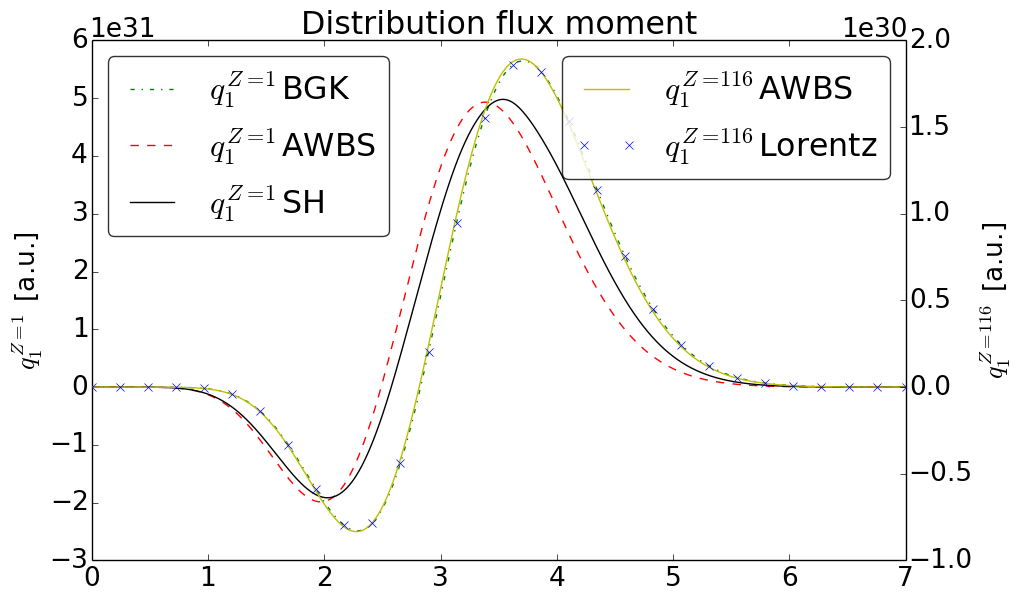
\includegraphics[width=0.5\textwidth]{q1s.png}
    \end{tabular}
  \caption{  
  The~flux velocity moment of the~anisotropic part of the~electron distribution 
  function in low $\Zbar=1$ and high $\Zbar=116$ plasmas in diffusive regime. 
  In the~case of $\Zbar = 1$ the~AWBS model matches very well 
  the~reference solution given by the~SH calculation \cite{SpitzerHarm_PR1953} 
  in comparison to the~BGK model. In the~case of $\Zbar = 116$ the~AWBS model
  aligns exactly with the~Lorentz gas approximation as expected. 
  The~BGK and the~SH curves are not shown for $\Zbar = 116$, but also 
  correspond to the~Lorentz gas distribution function.
  }
  \label{fig:q1s_summary}
  \end{center} 
\end{figure}

%At last, we provide a~quantitative information with respect to the~dominant 
%velocity of electrons contributing to the~heat flux. In the~high $\Zbar$ case
%all the~models give 3.7$\times \vth$, while SH solution gives 3.5$\times \vth$
%and AWBS 3.4$\times \vth$ in the~case of low $\Zbar$ plasmas, thus showing 
%the~right tendency of the~maximum velocity shift modeled by the~modified AWBS
%collision operator \eqref{eq:AWBS_model}.
%\begin{itemize} 
%  \item Point out the~behavior of the~maximum velocity of $q_1$, Lorentz 3.71, SHZ1 3.53, AWBSZ1 3.39.
%\end{itemize}


\section{The AWBS nonlocal transport model of electrons}
\label{sec:AWBSnonlocal}

In order to define a~nonlocal transport model of electrons, 
we use the~AWBS collision operator and the~P1 angular 
discretization of the~electron distribution function
\begin{equation}
  \tilde{\ft}(\vect{x}, \vn, \vmag) = 
  \fzero(\vect{x}, \vmag) + \vn\cdot\fone(\vect{x}, \vmag) , 
  \label{eq:P1approximation}
\end{equation}
consisting of the~isotropic part represented by the zeroth angular moment 
$\fzero = \frac{1}{4\pi}\int_{4\pi} \tilde{\ft} \dI\vn$ 
and the~directional part represented by the~first angular moment 
$\fone = \frac{3}{4\pi}\int_{4\pi} \vn
\tilde{\ft} \dI\vn$, where $\vn$ is the~transport direction.
%It should be noticed, that \eqref{eq:P1approximation} represents 
%a~multi-dimensional equivalent to \eqref{eq:f_approximation}, where 
%the~following relations between the~spherical harmonics method
%and the~moments method hold $\ft^0 = \frac{\fzero}{4\pi}$ and 
%$\ft^1 = \frac{3}{4\pi}|\fone|$.
Then, the~first two angular moments
\cite{Shkarofsky_Particle_Kinetics_book_1966_24} applied to the~stationary 
form of 
\eqref{eq:kinetic_equation} with collision operator \eqref{eq:AWBS_model} 
(extended by \eqref{eq:qAWBS_approximation}) lead to the~model equations
\begin{eqnarray}
  \vmag\frac{\nue}{2}\pdv{}{\vmag}\left(\fzero - \fM \right) &=&
  \frac{\vmag}{3}\nabla\cdot\fone + \frac{\qe}{\me}\frac{\E}{3}\cdot\left(
  \pdv{\fone}{\vmag} + \frac{2}{\vmag}\fone\right) , 
  \nonumber \\
  \label{eq:AP1f0}\\
  \vmag\frac{\nue}{2}\pdv{\fone}{\vmag}
  - \nuscat\fone &=& 
  \vmag\nabla\fzero + 
  \frac{\qe}{\me}\E\pdv{\fzero}{\vmag} 
  +\frac{\qe\B}{\me c}\vect{\times} \fone
  ,
  \nonumber \\
  \label{eq:AP1f1}
\end{eqnarray}
where $\nuscat = \nuei + \frac{\nue}{2}$. The system of equations 
\eqref{eq:AP1f0} and \eqref{eq:AP1f1} is called the~{\bf AP1 model} 
(AWBS + P1).  

The~AP1 model gives us information about the~electron distribution function 
%and
%a~macroscopic interpretation of the~microscopic EDF properties is of great
%importance 
providing a~bridge between kinetic and fluid description of 
plasma. For example the~\textit{flux} quantities as 
electric current and heat flux due to the~motion of electrons
\begin{equation}
  \vect{j} = \frac{4\pi}{3}\qe \int \vmag \fone \vmag^2\dI\vmag,~~ 
  \vect{q}_h = \frac{4\pi}{3}\frac{\me}{2} \int \vmag^3 \fone \vmag^2\dI\vmag,
  \nonumber
\end{equation}
where $\dI\tilde{\vmag} = \vmag^2\dI\vmag$ 
the~spherical coordinates metric,
are based on corresponding velocity moments (integrals) of the~first angular 
moment of EDF. Consequently, the~explicit formula for the~first angular moment
from \eqref{eq:AP1f1} 
%(the~inversion inspired by \cite{Shkarofsky_1979_73})
proves to be extremely useful
\begin{equation}
  \fone = \frac{\nuscat^2 \vect{F}^* + \omegaB~\omegaB\cdot\vect{F}^* 
  - \nuscat~\omegaB \vect{\times} \vect{F}^*}{\nuscat (\omegaB^2 + \nuscat^2)}
  ,
  \label{eq:f1_explicit}
\end{equation} 
because it provides a~valuable 
information about the~dependence of macroscopic \textit{flux} quantities on
electric and magnetic fields in plasma, 
where $\omegaB = \frac{\qe\B}{\me c}$ is the~electron gyro-frequency and 
$\vect{F}^* = \vmag\frac{\nue}{2}\pdv{\fone}{\vmag} - \vmag\nabla\fzero 
 - \frac{\qe}{\me}\E\pdv{\fzero}{\vmag}$.

\subsection{Nonlocal Ohm's Law}
\label{sec:Efield}
The~expression \eqref{eq:f1_explicit} becomes extremely useful when used
to describe the~electron fluid momentum, i.e. the~current velocity moment
%\begin{equation}
%  \vect{j}_{(f, \E, \B)} = \qe \int \vmag \fone \vmag^2 \dI \vmag
%  .
%  \nonumber
%\end{equation}
%\begin{multline}
%  \vect{j}_{(f, \E, \B)} = \qe \int \vmag \fone \vmag^2~\dI \vmag = \\
%  - \frac{\qe^2}{\me} \int \vmag \frac{\nuei^2 \E^* 
%  + \omegaB~\omegaB\cdot\E^* - \nuei~\omegaB \vect{\times} \E^*}
%  {\nuei (\omegaB^2 + \nuei^2)}~\dI \tilde{\vmag} ,
%  \nonumber %\label{eq:NonlocalOhm}
%\end{multline}
%where $\E^* = \E~\pdv{\fzero}{\vmag} + \frac{\me}{\qe}\vmag \nabla \fzero$ 
%is the~effective electric field in plasma. 
can be written as
\begin{equation}
  \vect{j}_{(f, \E, \B)} = \Iohm\pdv{\fzero}{\vmag}\E 
  + \frac{\me}{\qe} \Iohm\left(\vmag \nabla \fzero 
  - \vmag\frac{\nue}{2}\pdv{\fone}{\vmag} \right)  
  ,
  \label{eq:NonlocalOhm}
\end{equation}
where we used the~following notation 
$\Iohm\vect{g} = - \frac{4\pi \qe^2}{3 \me} \int \vmag \frac{\nuscat^2 \vect{g} 
  + \omegaB~\omegaB\cdot\vect{g} - \nuscat~\omegaB \vect{\times} \vect{g}}
  {\nuscat (\omegaB^2 + \nuscat^2)}~\vmag^2 \dI \vmag$ showing 
how the~operator $\Iohm$
acts on a~general vector field $\vect{g}$.
We refer to 
\eqref{eq:NonlocalOhm} as to the~{\bf nonlocal Ohm's law}.
The~need for a~nonlocal Ohm's law to accurately capture magnetic field 
advection by the~Nernst effect has previously been demonstrated 
\cite{Luciani85, Ridgers08, Brodrick18}, although a~full investigation 
of how well our new Ohm's law captures this is beyond 
the~scope of this article. 
The~proper high $\Zbar$ ($\nue \ll \nuei$) local asymptotic to 
the~standard Ohm's law  
can be found when $\fzero\rightarrow\fM$ and weak magnetization 
($\omegaB \ll \nuei$) is considered. Then \eqref{eq:NonlocalOhm} simplifies to
\begin{multline}
  \vect{j} =- \frac{\qe^2}{\me} \int \frac{\vmag^3}{\nuei}
  \left( \E~\pdv{\fM}{\vmag} + \frac{\me}{\qe}\vmag \nabla \fM \right)
  ~\dI \vmag =\\
  \frac{16\sqrt{\frac{2}{\pi}}\qe^2 \kB^\frac{3}{2} \Te^\frac{3}{2}}{\me^\frac{5}{2} \Gamma\Zbar}
  \left[\E - \frac{\frac{5}{2} \ed \kB \nabla \Te 
  + \nabla \ed \kB \Te}{\qe \ed}  \right] 
  ,
  \label{eq:AsymptoticOhm}
\end{multline}
which can be directly compared to the~local fluid theory 
%represented by the~\textit{generalized Ohm's law} 
\begin{equation}
  \E = \matr{\sigma}(\fzero)^{-1} \vect{j} 
  - \frac{\nabla P (\fzero)}{\qe \ed}
  \xrightarrow{\fzero \rightarrow \fM}
  \E_{l} = \frac{\vect{j}}{\sigma_{l}}
  + \frac{\nabla p_e - \vect{R}_{\Te}}{\qe \ed} 
  ,
  \label{eq:GeneralOhm} 
\end{equation}
while addressing properly the~local electric field $\E_{l}$ given by
the~pressure $p_e = \ed \kB \Te$,
the~thermal force $\vect{R}_{\Te} = - \frac{3}{2} \ed \kB \nabla \Te$ 
and the~local electrical conductivity 
$\sigma_{l} = 16\sqrt{\frac{2}{\pi}}\qe^2 \kB^\frac{3}{2} \Te^\frac{3}{2}
/ \me^\frac{5}{2} \Gamma\Zbar$ \cite{Braginskii_1965_3}.
In \eqref{eq:GeneralOhm} we defined the~nonlocal electrical tensor conductivity 
\begin{equation}
  \matr{\sigma} = \Iohm\pdv{\fzero}{\vmag}
  ,
  \label{eq:NonlocalSigma}
\end{equation}
and the~nonlocal microscopic force
\begin{equation}
  \nabla P = \matr{\sigma}^{-1}\me\ed \Iohm\vmag \nabla \fzero
  ,
  \label{eq:NonlocalGradP}
\end{equation}
based on \eqref{eq:NonlocalOhm}.

The~local dependence of the~AP1 current \eqref{eq:AsymptoticOhm} 
on electric field and gradients of $\ed$ and $\Te$ clearly demonstrates, 
that \eqref{eq:GeneralOhm} is a~local version of \eqref{eq:NonlocalOhm}.
This also implies that \eqref{eq:NonlocalOhm} provides a~very important 
physics related to the~magnetic field source in terms of nonlocal 
Biermann battery,
since the~curl on the~electric field 
\eqref{eq:GeneralOhm} gives
\begin{equation}
  \nabla\vect{\times} \frac{\nabla P}{\qe \ed} 
  \xrightarrow{\fzero \rightarrow \fM} 
  \nabla\vect{\times} \frac{\nabla p_e - \vect{R}_{\Te}}{\qe \ed} =
  \frac{\kB}{\qe\ed}\nabla \Te \vect{\times}\nabla \ed
  .
  \label{eq:NonlocalBiermann}
\end{equation}
The~nonlocal Biermann battery equivalent \eqref{eq:NonlocalBiermann} 
can lead to a~spontaneous magnetic field generation under uniform 
density plasma profile as has been shown in \cite{Kingham_PRL2002}.
%even in the~collisional case not considered PIC simulations

A~local version of the~{\bf nonlocal Ohm's law} \eqref{eq:NonlocalOhm} 
compared to the~\textit{generalized Ohm's law} \eqref{eq:GeneralOhm} when
a~magnetic field is applied would require a~much more delicate analysis and 
we leave it as a~future complementary work.

%It should be noted, that $\nue$-related terms in \eqref{eq:f1_explicit} 
%have been omitted in \eqref{eq:NonlocalOhm}, 
%since the~e-e collisions do not contribute 
%(cancel out when integrated over velocity) to the~momentum
%change, i.e. 
%$\int \vmag \left( \vmag\frac{\nue}{2}\pdv{\fone}{\vmag}
%  - \frac{\nue}{2}\fone\right) \dI\tilde{\vmag} = 0$.

\begin{comment} % Ohm's law with B.
\begin{eqnarray} 
  \E &=&  
  \frac{\nabla p_e - \vect{R}_{\Te}}{\qe \ed}
  +~~~~~~~~ 
  \frac{\vect{j}}{\sigma} 
  ~~~~~~-~~~~~~ 
  \frac{\vect{j}\vect{\times}\B}{\qe\ed c} 
  ,
  \nonumber \\
  %\E 
  %&=& 
  %\frac{\int \vmag^2 \nabla \fzero \vmag^2\, \dI \vmag}
  %{\int \vmag \pdv{\fzero}{\vmag} \vmag^2\, \dI \vmag}
  %+  
  %\frac{\int \vmag \nuei\fone \vmag^2\, \dI \vmag}
  %{\int \vmag \pdv{\fzero}{\vmag} \vmag^2\, \dI \vmag} 
  %+ 
  %\frac{\int \vmag \fone\times\B \vmag^2\, \dI \vmag}
  %{\int \vmag \pdv{\fzero}{\vmag} \vmag^2\, \dI \vmag} 
  %.
  %\nonumber
  \frac{\qe}{\me}\E 
  &=& 
  \frac{\int \vmag^2 \nabla \fzero~\dI \tilde{\vmag}}
  {\int \vmag \pdv{\fzero}{\vmag}~\dI \tilde{\vmag}}
  +  
  \frac{\int \vmag \nuei\fone~\dI \tilde{\vmag}}
  {\int \vmag \pdv{\fzero}{\vmag}~\dI \tilde{\vmag}} 
  + 
  \frac{\qe\int \vmag \fone\vect{\times}\B~\dI \tilde{\vmag}}
  {\me c \int \vmag \pdv{\fzero}{\vmag}~\dI \tilde{\vmag}} 
  .
  \nonumber
\end{eqnarray}
\end{comment} % Ohm's law with B.

\subsection{AWBS Nonlocal Magneto-Hydrodynamics}
\label{sec:ANTH}
The~\textit{AWBS nonlocal~magneto-hydrodynamic~model} (Nonlocal-MHD)
refers to two~temperature single-fluid hydrodynamic model 
extended by a~kinetic model of electrons using the~AWBS transport equation,
which provides a~direct coupling between hydrodynamics and Maxwell equations.

Mass, momentum density, and total energy 
$\rho$, $\rho\vect{u}$, and 
$E = \frac{1}{2}\rho\vect{u}\cdot\vect{u} + 
 \rho \varepsilon_i + \rho \varepsilon_e$, 
where $\rho$ is 
the~density of plasma, $\vect{u}$ the~plasma fluid velocity, $\varepsilon_i$ 
the~specific internal ion energy density, 
and $\varepsilon_e$ the~specific internal 
electron energy density,
are modeled by the~Euler equations in the~Lagrangian frame 
\cite{Holec_DGBGKT_2016, Holec_PoPNTH2018}
\begin{eqnarray}
 \frac{\dI \rho}{\dI t} &=& - \rho\nabla\cdot\vect{u}
 , 
 \label{eq:NTH_rho}\\
 \rho\, \frac{\dI \vect{u}}{\dI t} &=& - \nabla (p_i + p_e) 
 + \vect{j}_{(f, \E, \B)} \vect{\times}\B
 ,  
 \label{eq:NTH_v}\\
 \rho~C_{V_i}\frac{\dI \Ti}{\dI t} 
 &=& 
 \left(\rho^2 C_{\Ti} - p_i\right)\nabla\cdot\vect{u} 
 - G(\Ti - \Te)
 ,  
 \label{eq:NTH_Ti}\\
 \rho~C_{V_e} \frac{\dI \Te}{\dI t}
  %+ \frac{\dI \epsilon_R}{\dI t} 
  &=& 
 \left(\rho^2 C_{\Te} - p_e \right) \nabla\cdot\vect{u}  
 + G(T_i - \Te)
 \nonumber\\ 
 && - \nabla\cdot\vect{q}_{h(f, \E, \B)} + Q_{\text{IB}} 
 , 
 \label{eq:NTH_Te}
\end{eqnarray}
where $\Ti$ is the~temperature of ions, $\Te$ the~temperature of electrons,
$p_i$ the~ion pressure, $p_e$ the~electron pressure,
$\vect{q}_h$ the~heat flux, $Q_{\text{IB}}$ the~inverse-bremsstrahlung laser 
absorption (which can also distort the distribution function away from 
a~Maxwellian \cite{Langdon80}, strongly modifying the~transport 
\cite{Ridgers08_2}, an~effect which will not be considered further here) and 
$G = \rho C_{V_e} \nuei$ is 
the~ion-electron energy exchange rate. 
The~thermodynamic closure terms 
$p_e$, $p_i$, 
$C_{V_i} = \frac{\partial \varepsilon_i}{\partial \Ti}$, 
$C_{\Ti} = \pdv{\varepsilon_i}{\rho}$,
$C_{V_e} = \frac{\partial \varepsilon_e}{\partial \Te}$, 
$C_{\Te} = \pdv{\varepsilon_e}{\rho}$
%$\frac{\partial \varepsilon_e}{\partial T_e}$,
%$\frac{\partial \varepsilon_i}{\partial T_i}$,
%$\frac{\partial \varepsilon_e}{\partial \rho}$,
%$\frac{\partial \varepsilon_i}{\partial \rho}$ 
are obtained from an~equation of state (EOS), e.g.
the~SESAME equation of state tables
\cite{T4_SESAME_83, Lyon_SESAME_EOS_database-TechRep-92}.

The~magnetic and electric fields are modeled by Maxwell equations
\begin{eqnarray}
  \frac{1}{c}\frac{\partial \B}{\partial t} &=& - \nabla\vect{\times}\E
  ,
  \label{eq:Faraday} \\
  \frac{1}{c}\frac{\partial \E}{\partial t} &=& \nabla\vect{\times}\B - \frac{4\pi}{c}
  \vect{j}_{(f, \E, \B)}
  ,
  \label{eq:Ampere}
  %\frac{4\pi}{c}
  %\vect{j}(f, \vect{E}) &=& \nabla\vect{\times}\vect{B} ,
\end{eqnarray}
where the~initial state of $\B$ and $\E$ obeys the~Gauss's law.

We have explicitly written the~current and heat flux as dependent on
electron kinetics, represented by the~electron distribution function $f$,
and electric and magnetic fields. In principal, $\vect{j}_{(f, \E, \B)}$
and $\vect{q}_{h(f, \E, \B)}$ can be referred to as the~\textit{kinetic closure}
and is provided by the~{\bf AP1 model} \eqref{eq:AP1f0} and \eqref{eq:AP1f1}.
%where $\fM$ is given on the~spatial profile of $\Te$ 
%governed by \eqref{eq:NTH_Te}.
%All quantities are defined in the~fluid frame in the aforementioned 
%Nonlocal-MHD model.

\subsection{Numerical Implementation of the AWBS Electron Kinetics}
\label{sec:Numerics}

It is well known, that as the~electron transport exhibits a~quasi-steady
behavior, the~same holds for the~electric field in \eqref{eq:Ampere} on 
the~time scale of the~fluid. Consequently, Ampere's law \eqref{eq:Ampere} 
takes a~quasi-steady form 
$\frac{4\pi}{c} \vect{j}_{(f, \E, \B)} = \nabla\vect{\times}\B$
when used in hydrodynamics. Proceeding further, one can make use of 
the~{\bf nonlocal Ohm's law} \eqref{eq:NonlocalOhm} to write 
a~\textit{fully kinetic form of Ampere's law} 
governing the~electric field $\E$
\begin{equation}
  \Iohm\pdv{\fzero}{\vmag}\E 
  + \frac{\me}{\qe} \Iohm\vmag \nabla \fzero = 
  \frac{c}{4\pi} \nabla\vect{\times}\B 
  .
  \label{eq:AmpereKinetic}
\end{equation}

In order to solve the~kinetics of electrons, we adopt a~high-order 
finite element discretization 
\cite{Dobrev_Kolev_Rieben-High-order_curvilinear_finite_element_methods_for_Lagrangian_hydrodynamics, mfem-library} 
of the~model equations \eqref{eq:AP1f0}, \eqref{eq:AP1f1}, 
\eqref{eq:AmpereKinetic}
\begin{eqnarray}
  \matr{M}^{L_2}_{_{(\frac{\vmag\nue}{2})}}\cdot\ddv{\vfzero}{\vmag} 
  - \matr{V}^{L_2}_{_{(\frac{\qe\E}{3\me})}}\cdot\ddv{\fone}{\vmag}
  &=&
  \matr{D}^{L_2}_{_{(\frac{\vmag}{3})}}\cdot\fone 
  + \matr{M}^{L_2}_{_{(\frac{2\qe\E}{3\me\vmag})}}\cdot\fone
  \nonumber \\ 
  &&+ \vect{b}^{L_2}_{_{(\frac{\vmag\nue}{2}\pdv{\fM}{\vmag})}}, 
  \label{eq:FEMAP1f0}
  \\
  \matr{M}^{H_1}_{_{(\frac{\vmag\nue}{2})}}\cdot\ddv{\fone}{\vmag}
  - \matr{V}^{H_1}_{_{(\frac{\qe\E}{\me})}}\cdot\ddv{\vfzero}{\vmag}
   &=& 
  \matr{G}^{H_1}_{_{(\vmag)}}\cdot\vfzero 
  + \matr{M}^{H_1}_{_{(\nuscat)}}\cdot\fone 
  \nonumber \\
  && + \matr{C}^{H_1}_{_{(\frac{\qe\B}{\me c}\vect{\times})}}\cdot\fone
  ,
  \label{eq:FEMAP1f1}\\
  \matr{J}^{ND}_{_{(\pdv{\fzero}{\vmag})}}\cdot\E 
  &=& 
  \matr{JG}^{ND}_{_{(\frac{\me\vmag}{\qe})}}\cdot\vfzero
  + \vect{b}^{ND}_{_{(\frac{c}{4\pi} \nabla\vect{\times}\B)}} 
  ,
  \nonumber \\
  \label{eq:FEMAmpereKinetic}
\end{eqnarray}
where the~continuous differential operators are represented by standard 
discrete analogs (matrices of bilinear forms) 
$\matr{M}, \matr{G}, \matr{D}, \matr{V}, \matr{C}$, i.e. mass, gradient, 
divergence, vector field dot product, and vector field curl, and
by $\matr{J}, \matr{JG}$ matrices specific to {\bf nonlocal Ohm's law} 
\eqref{eq:NonlocalOhm}. The~linear form $\vect{b}$ represents sources, i.e.
temperature $\Te$ via $\pdv{\fM}{\vmag}$ and the~curl of 
the~magnetic field $\B$. These finite element discrete analogs are defined
on piece-wise continuous $L_2$ finite element space (domain of $\vfzero$),
continuous $H_1$ finite element space (domain of $\fone$) 
\cite{Dobrev_Kolev_Rieben-High-order_curvilinear_finite_element_methods_for_Lagrangian_hydrodynamics}, 
and Nedelec finite element space (domain of $\E$). We do not show their
definitions since it is out of the~scope of this article. 

The~strategy of solving 
\eqref{eq:FEMAP1f0} and \eqref{eq:FEMAP1f1} resides in integrating 
$\ddv{\vfzero}{\vmag}$
and $\ddv{\fone}{\vmag}$ along the~velocity magnitude. 
This is done by starting the~integration
from the~maximum  velocity 
($\vmag = 7 \vth^{max}$ is a~sufficiently high limit) 
to zero velocity using the~Implicit Runge-Kutta method. The~value
$\vth^{max}$ equals the~electron thermal velocity corresponding to the~maximum 
electron temperature in the~current profile of plasma.
It should be noted, that the~backward integration concept is crucial for 
the~model, since it corresponds to the~deceleration of electrons due to 
collisions \cite{Touati_2014}. Consequently, we refer to 
\textit{decelerating} AP1 model, which however, leads to the~limitation of 
the~electric field described in \appref{app:AP1limit}. 


\section{Benchmarking the~AWBS nonlocal transport model}
\label{sec:BenchmarkingAWBS}
Having shown several encouraging properties of the~AWBS transport 
equation defined by \eqref{eq:AWBS_model} under local diffusive conditions
in \secref{sec:DiffusiveKinetics}, this section focuses on analyzing 
its behavior under nonlocal plasma conditions, extensively investigated 
in numerous publications 
\cite{Malone_1975_15, Colombant_PoP2005, Bell_1981_83, LMV_1983_7, Brantov_Nonlocal_electron_transport_1998, Schurtz_2000, Sorbo_2015}.
A~variety of tests suitable for benchmarking the~nonlocal electron 
transport models have been published 
\cite{Epperlein_PoFB1991, marocchino2013, Sorbo_2015, 
Sorbo_2016, Sherlock_PoP2017, Brodrick_PoP2017}, we focus on 
conditions relevant to inertial confinement fusion plasmas generated by lasers.

We show results of our implementation of the~AP1 nonlocal transport model 
presented in \secref{sec:AWBSnonlocal} benchmarked against simulation results 
provided by a~rather complete set of kinetic models with varying complexity. 
The~most reliable models represents a~collisional Particle-In-Cell
code Calder \cite{Lefebvre_NF2003, Perez_PoP2012} resolving 
the~plasma frequency time scale, and a~standard VFP codes
Aladin and Impact \cite{Kingham_JCP2004}.
In addition, we compare the~SNB nonlocal transport model \cite{Schurtz_2000} 
used in hydrodynamic codes. 
That is a~first time when a~collisional PIC code is used
for benchmarking of nonlocal electron transport models. 

%%% CEA contribution starts
\textbf{Calder PIC code}

The~particle evolution in the~phase-space, including small angle 
binary collisions, is described with 
the~Maxwell equations \eqref{eq:Faraday}, \eqref{eq:Ampere}
%\begin{eqnarray}
%&&\nabla\cdot \mathbf{E}=\sum_\alpha \frac{q_\alpha}{\varepsilon_0} n_{\alpha},\\
%&&\nabla\cdot \mathbf{B}=0,\\
%&&\nabla\vect{\times} \mathbf{E}+\frac{\partial \mathbf{B}}{\partial t}=0,\\
%&&\nabla\vect{\times} \mathbf{B}-\mu_0\varepsilon_0\frac{\partial \mathbf{E}}{\partial t}=\mu_0\sum_\alpha\mathbf{j}_{\alpha},\label{maxw}
%\end{eqnarray}
coupled with the~ion and electron Vlasov equations with 
the~Landau-Beliaev-Budker collisions integral (LBB)
\cite{Landau_1936, Beliaev_SPD1956} 
\begin{multline}
\frac{\partial f_\alpha}{\partial t}+\mathbf{v}\cdot\nabla_{\mathbf{x}}f_\alpha+q_\alpha\left(\mathbf{E}+\mathbf{v}\vect{\times}\mathbf{B}\right)\nabla_{\mathbf{p}}f_\alpha =
\\
C_{LBB}(f_\alpha,f_\alpha)+\sum_\beta C_{LBB}(f_\alpha,f_\beta)
.
\end{multline}
The LBB collision integral takes the~form
\begin{multline}
C_{LBB}(f_\alpha,f_\beta)=
\\
-\frac{\partial}{\partial \mathbf{p}}\cdot\frac{\Gamma_{\alpha\beta}}{2}\left[\int \mathbf{U}(\mathbf{p},\mathbf{p}^\prime)\cdot(f_\alpha\nabla_{\mathbf{p}^\prime}f_\beta^\prime-f_\beta^\prime\nabla_{\mathbf{p}}f_\alpha)\right]d^3\mathbf{p}^\prime
,
\label{eq:LBB_model}
\end{multline}
where its relativistic kernel reads
$\mathbf{U}(\mathbf{p},\mathbf{p}^\prime)=\frac{r^2/\gamma\gamma^\prime}{(r^2-1)^{3/2}}$ 
$\left[(r^2-1)\mathbf{I}-\mathbf{p}\otimes\mathbf{p}-\mathbf{p}^\prime\otimes\mathbf{p}^\prime+r(\mathbf{p}\otimes\mathbf{p}^\prime+\mathbf{p}^\prime\otimes\mathbf{p})\right]$
with $\gamma=\sqrt{1+\mathbf{p}^2}$, $\gamma^\prime=\sqrt{1+\mathbf{p}^{\prime 2}}$ and $r=\gamma\gamma^\prime-\mathbf{p}\cdot\mathbf{p}^\prime$. 
The momemtum $\mathbf{p}_\alpha$ ($\mathbf{p}_\beta$) is normalized to 
$m_\alpha c$ (resp. $m_\beta c$). The~collision operator \eqref{eq:LBB_model} 
tends to \eqref{eq:LFP_model} in the non-relativistic limit.
%described in Appendix~\ref{app:CalderKinetics}. 
%The~latter is the~relativistic version of the~collision operator 
%introduced in \eqref{eq:LFP_model}. 
The aforementioned model is solved in 3D by the PIC code CALDER. 
\cite{Lefebvre_NF2003, Perez_PoP2012}.

\textbf{Impact and Aladin VFP codes}

PIC simulations are extremely expensive as the~collisions require description 
of the~velocity space in 3 dimensions. Yet, a~reduction of dimensions can be 
done by developing the~distribution function in a~Cartesian tensor series, 
equivalent to expansion in the spherical harmonics \cite{Johnston_PR1960}.
%as follows:\textit{CPR comment - Cartesian tensors are the same as spherical harmonics to first order}
%\begin{equation}
%  f(t,\mathbf{x},\vv) = f_0(t,\mathbf{x},\vmag) 
%  + \vn\cdot \vect{f}_1(t,\mathbf{x},\vmag)
%  +\vn\otimes\vn:\matr{f}_2(t,\mathbf{x},\vmag)+... .
%  \label{Pn}
%\end{equation}
%where $v=|\mathbf{v}|$, $\Omega=\mathbf{v}/v$. 
%A P$_n$ model refers to 
%neglecting orders higher than $\matr{f}_n$. 
The~first order form corresponds to the~P1 approximation 
\eqref{eq:P1approximation} and coupled with
%distribution function 
%approximation $f(t,\mathbf{x},\vv)\approx f_0(t,\mathbf{x},\vmag)
%+\vn\cdot \vect{f}_1(t,\mathbf{x},\vmag)$ coupled with 
the~Landau-Fokker-Planck collisional operator 
\eqref{eq:LFP_model} leads to the P$_1$-VFP model 
\cite{Johnston_PR1960, Kingham_JCP2004}:
\begin{eqnarray}
\frac{\partial \fzero}{\partial t}+\frac{\vmag}{3}\nabla \cdot \fone
+\frac{\qe}{3\me\vmag^2}\frac{\partial}{\partial \vmag}(\vmag^2\E\cdot \fone)
&=&
C^0_{ee}(\fzero) ,
 \label{eq:P1f0_Aladin}\\
\frac{\partial \fone}{\partial t}+\vmag\nabla \fzero
+ \frac{\qe\E}{\me}\frac{\partial \fzero}{\partial \vmag}
+\frac{\qe\B}{\me}\vect{\times} \fone 
&=&
- \nuei\fone .
\label{eq:P1f1_Aladin}
\end{eqnarray}
where only the~isotropic part of the~distribution function in 
the~e-e collision integral \eqref{eq:LFP_model} is used
\begin{eqnarray} 
C^0_{ee}(\fzero) &=& \frac{\Gamma}{v^2}\frac{\partial}{\partial \vmag}
\left[C(f_0)f_0+D(\fzero)\frac{\partial \fzero}{\partial \vmag}\right] ,
\label{eq:C0_collision_operator}
\\
C(\fzero(\vmag)) &=& 4\pi\int_0^\vmag \fzero(u) u^2 \dI u ,
\nonumber
\\
D(\fzero\vmag)) &=& \frac{4\pi}{\vmag}\int_0^\vmag u^2\int_u^\infty w \fzero(w) 
\dI w \dI u .
\nonumber
\end{eqnarray}

The~codes Impact and Aladin solve the system \eqref{eq:P1f0_Aladin} 
and \eqref{eq:P1f1_Aladin} with the Maxwell equations  
\eqref{eq:Faraday} and \eqref{eq:Ampere} in two spatial dimensions, 
assuming immobile ions.

The~model AP1 uses similar equations as Aladin
and Impact with the~difference, that AP1 describes the~steady-state 
electron distribution function with respect to the~ions,
and is using a~simplified (linear) collision operator inherently
coupled to ions via the~hydrodynamic equations.

%%% CEA contribution ends

\textbf{SNB approach}

Now considered as a~standard nonlocal electron transport models in hydrodynamic 
codes, SNB \cite{Schurtz_2000} represents an efficient P1 method based on
the~velocity dependent form of the~collision BGK operator. It uses EDF 
approximation representing deviation from the~local BGK theory
\begin{equation}
  \tilde{\ft} = 
  \fM + \delta\fzero 
  + \vn\cdot\left(\fone_M + \delta\fone\right) . 
  \label{eq:SNB_approximation}
\end{equation}
%where $\fone_M = - \xi\mfpei\left( \frac{\vmag^2}{2 \vth^2} - 4\right)\fM
%\frac{\nabla \Te}{\Te}$ is obtained from the~diffusive solution 
%\eqref{eq:BGK_approximation} with \eqref{eq:BGK_scaling}.
Equations for the~zero and first angular moments follow from 
the~electron transport equation with scaled collision operator 
\eqref{eq:BGK_scaling}
according to the~SNB approximation \eqref{eq:SNB_approximation} 
(similar to \eqref{eq:AP1f0} and \eqref{eq:AP1f1})
\begin{eqnarray}
  r_B \delta\fzero &=&
  - \frac{\vmag}{3}\nabla\cdot\delta\fone
  - \frac{\vmag}{3}\nabla\cdot\fone_M
  \nonumber\\ 
  &&\xcancel{- \frac{\qe}{\me}\frac{\E}{3}\cdot\left(
  \pdv{\fone_M}{\vmag} + \pdv{\delta\fone}{\vmag} 
  + \frac{2}{\vmag}\left(\fone_M + \delta\fone\right)\right)} , 
  \nonumber \\
  \label{eq:SNBf0}\\
  \frac{\nuei}{\xi}\delta\fone &=& - \vmag\nabla\delta\fzero 
  ~\xcancel{- \frac{\qe}{\me}\E\pdv{\delta\fzero}{\vmag}}
  %- \omegaB\vect{\times} \delta\fone } 
  \nonumber \\
  &&\underbrace{- \frac{\nuei}{\xi}\fone_M - \vmag\nabla\fM
  - \frac{\qe}{\me}\E\pdv{\fM}{\vmag}
  %- \omegaB\vect{\times} \fone_M
  }_{~~~~~~~~~~~~~=~0~defines~\fone_M} 
  %+\frac{\qe\B}{\me c}\vect{\times} \left(\fone_M + \delta\fone\right)
  ,
  \nonumber \\
  \label{eq:SNBf1}
\end{eqnarray}
where the~magnetic field was neglected, the~under-braced part
of \eqref{eq:SNBf1} when $\delta\fzero$ and $\delta \fone$ are zero
defines the~local anisotropic term
%where $\fone_M = \frac{\frac{\nuei^2}{\xi^2} \vect{F}_M 
%+ \omegaB~\omegaB\cdot\vect{F}_M - \frac{\nuei}{\xi}~\omegaB \vect{\times} 
%\vect{F}_M}{\frac{\nuei}{\xi} \left(\omegaB^2 + \frac{\nuei^2}{\xi^2}\right)}$
%, where $\vect{F}_M = -\vmag \left( \frac{\fM}{\ed}\nabla\ed 
%+ \left( \frac{\vmag^2}{2\vth^2} - \frac{3}{2}\right)
%\frac{\fM}{\Te}\nabla\Te - \frac{\qe \fM}{\me\vth^2}\E\right)$.
\begin{equation}
  \fone_M = -\xi\mfpei\fM\left( \frac{\nabla\ed}{\ed} 
+ \left( \frac{\vmag^2}{2\vth^2} - \frac{3}{2}\right)
\frac{\nabla\Te}{\Te} - \frac{\qe\E}{\me\vth^2}\right) ,
  \label{eq:f1M}
\end{equation}
%One should notice, that the~local
%EDF contribution cancels out in \eqref{eq:SNBf1} when the~electric field 
%adjusts to the~local Lorentz electric field \eqref{app_eq:BGK_Efield}. 
and the~efficiency of SNB resides in omitting the~electric field 
effect (crossed out terms in \eqref{eq:SNBf0} and \eqref{eq:SNBf1}), which
leads to a~simple diffusion equation for the~correction to the~isotropic 
part of the~distribution function
\begin{equation}
  \frac{1}{\mfpe^{SNB}}\delta\fzero 
  - \nabla\cdot\frac{\mfpei^{SNB}}{3}\nabla\delta\fzero =
  \nabla\cdot\frac{\xi\mfpei}{3}\fM\frac{\nabla \Te}{\Te}
  ,
  \label{eq:SNB_model}
\end{equation}
where $\frac{1}{\mfpei^{SNB}} = 
\frac{\nuei}{\xi\vmag} + \frac{|\qe\E|}{\frac{1}{2}\me\vmag^2}$ 
and $\mfpe^{SNB} = \frac{\vmag}{r_B \nue}$, and the~source term based on 
$\fone_M$ simplifies by avoiding the~electric field effect, density gradient 
and the~$\vmag$-dependent bracket in \eqref{eq:f1M}. The~missing
effect of $\E$ in \eqref{eq:SNB_model} is accounted for by 
an~isotropic scattering in definition of $\mfpei^{SNB}$ \cite{Schurtz_2000}.
Consequently, the~effect of the~electric field in SNB
is accounted for only via $\fone_M$, where the~electric field is
fixed to $\E_L$. 
%A~self consistent zero current condition 
%$\vect{j} = \qe \int \vmag (\fone_M + \delta\fone)~\dI\tilde{\vmag} = 0$ then
%defines the~actual value of the~electric field from \eqref{eq:SNBf1} as
%\begin{equation}
% \E = -\frac{\int \frac{\xi\vmag^2}{\nuei}\nabla
% \left(\fM + \delta\fzero\right)~\dI\tilde{\vmag}}
% {\int \frac{\xi\vmag}{\nuei}\frac{\qe}{\me}\pdv{\fM}{\vmag}
% ~\dI\tilde{\vmag} } 
% = \E_L - \frac{\int \frac{\vmag^2}{\nuei}\nabla
% \delta\fzero~\dI\tilde{\vmag}}
% {\frac{\qe}{\me}\int \frac{\vmag}{\nuei}\pdv{\fM}{\vmag}
% ~\dI\tilde{\vmag} } ,
% \label{eq:SNB_E} 
%\end{equation}

As shown previously, the~BGK collision operator \eqref{eq:BGK_scaling}
provides one free parameter $\zeta$.
We propose to use $\zeta = 2$ giving $r_B(\Zbar\gg1) = 2$ which agrees 
with $r=2$ in SNB formulation proposed in \cite{Brodrick_PoP2017} 
for the~case of ICF relevant plasma. We also have $r_B(\Zbar = 1) = 1.677$,
which means that our pure kinetic derivation of SNB varies just slightly
from a~constant value $r_B=2$ \cite{Brodrick_PoP2017}, yet it provides 
slightly better results. The~explicit form of the~anisotropic 
part of EDF then reads $\fone = \fone_M - \mfpei^{SNB}\nabla\delta\fzero$.

\begin{figure*}[htb]
  \begin{center}
    \begin{tabular}{cc}
      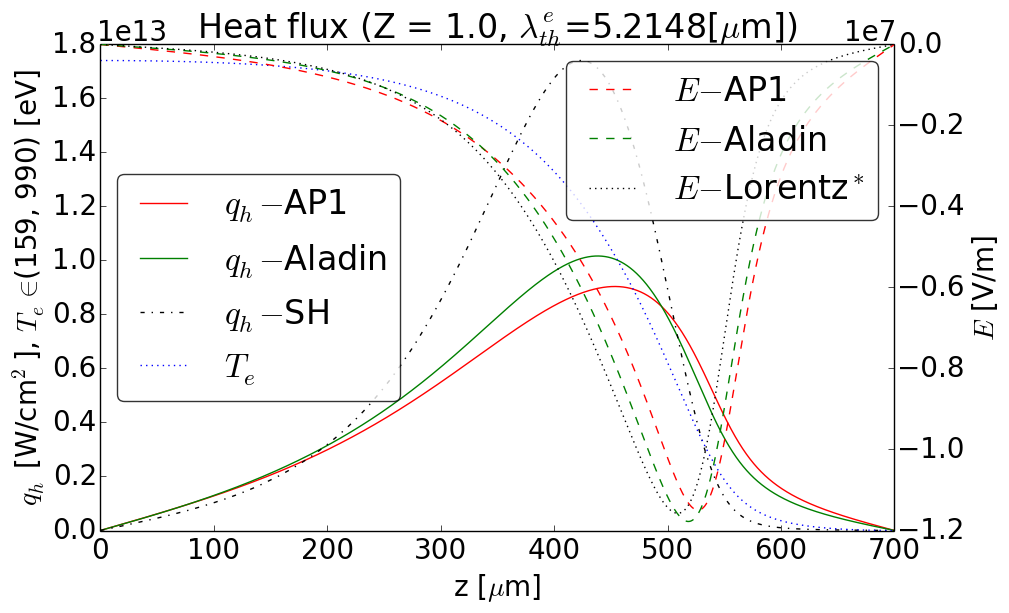
\includegraphics[width=\figscale\textwidth]{../VFPdata/C7_Aladin_case5_heatflux.png} 
	  &
      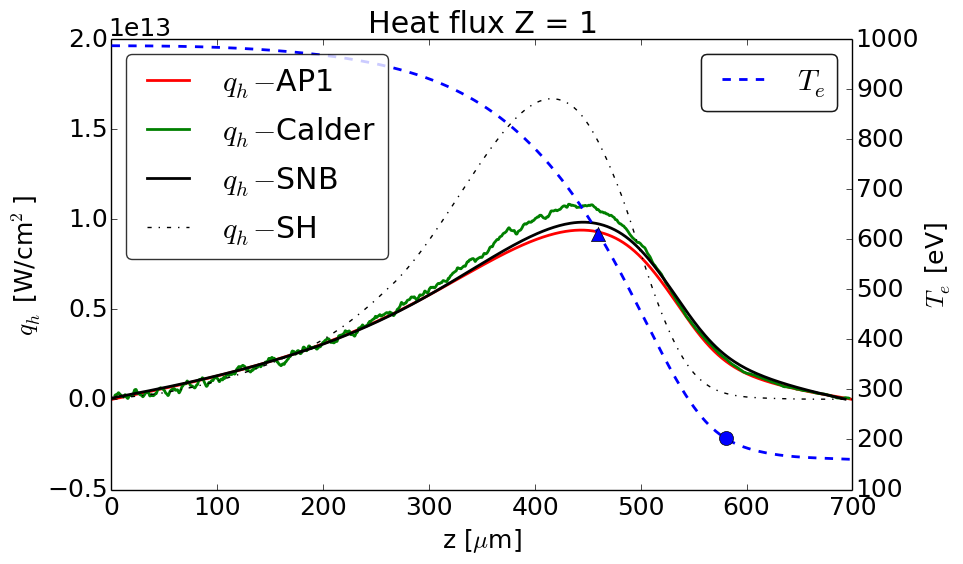
\includegraphics[width=\figscale\textwidth]{../VFPdata/C7_Calder_case5_heatflux.png} 
	  \\ 
      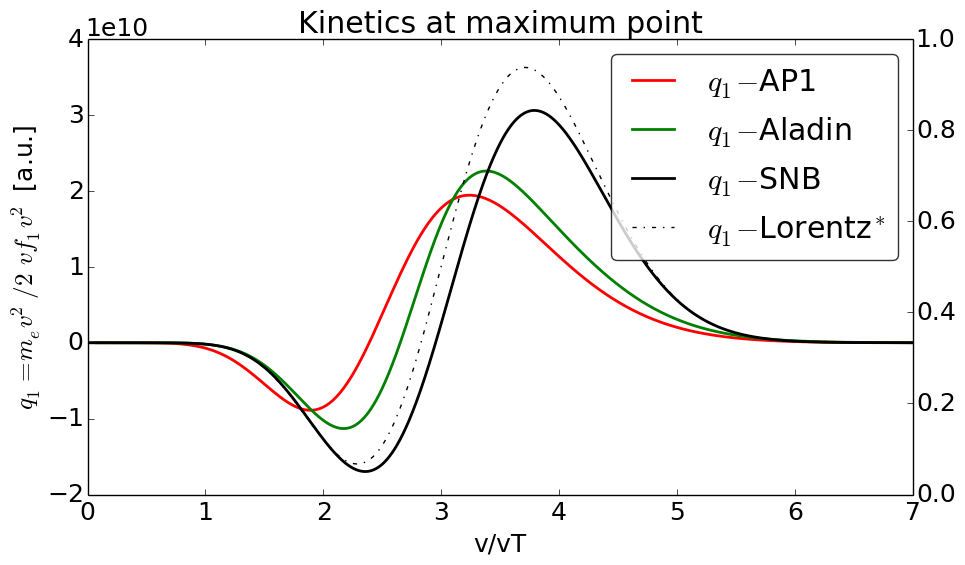
\includegraphics[width=\figscale\textwidth]{../VFPdata/C7_Aladin_case5_kinetics.png} 
	  &
      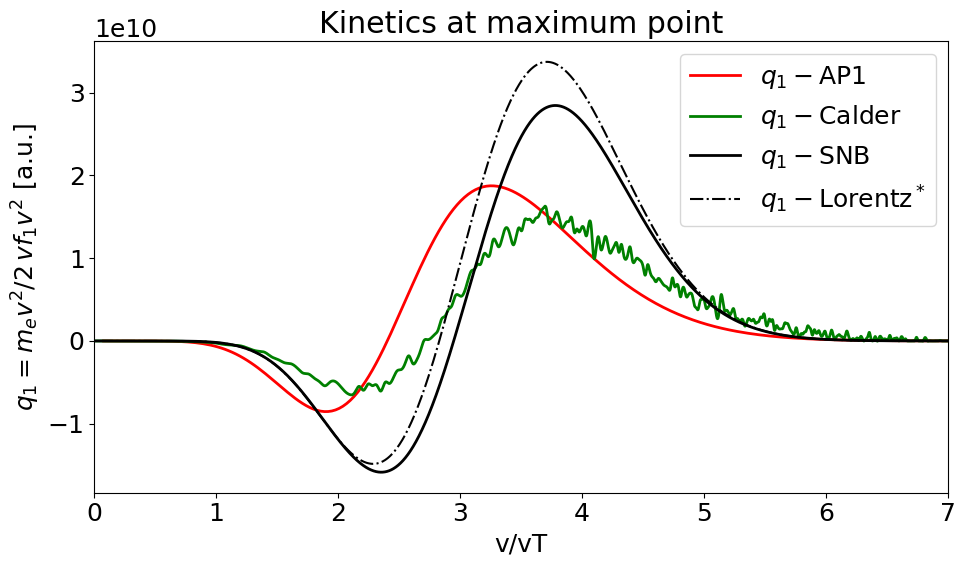
\includegraphics[width=\figscale\textwidth]{../VFPdata/C7_Calder_case5_kinetics.png} 
	  \\
	  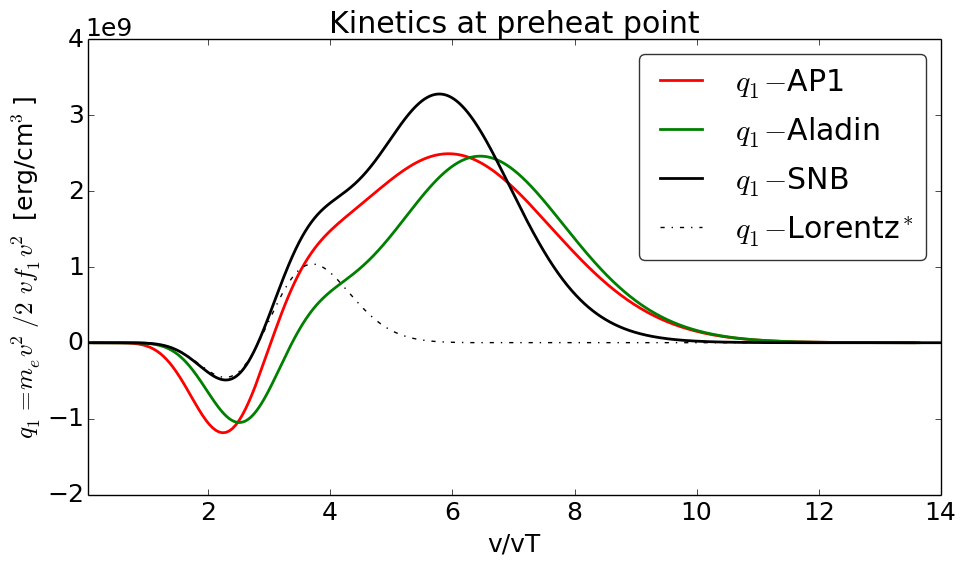
\includegraphics[width=\figscale\textwidth]{../VFPdata/C7_Aladin_case5_nonlocal_kinetics.png} 
      &
      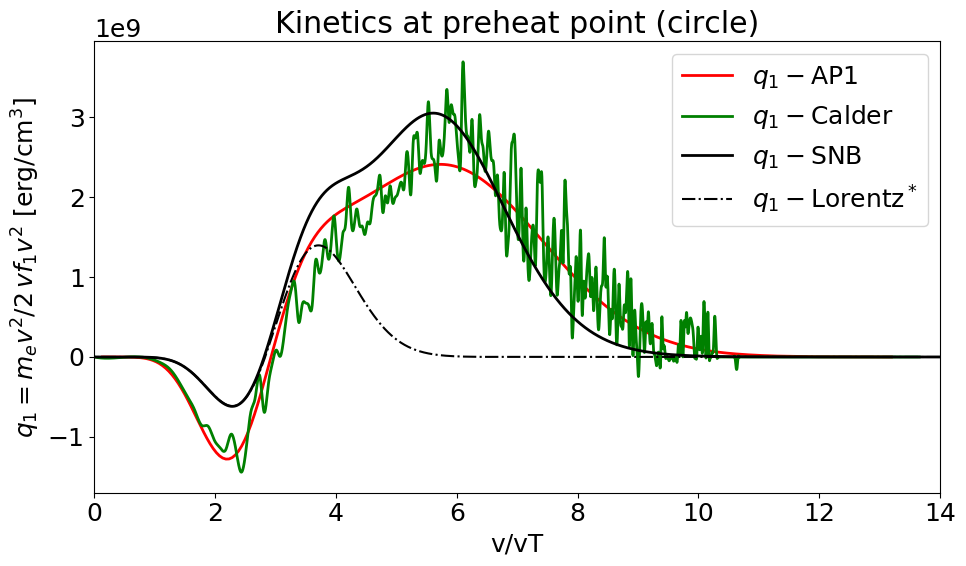
\includegraphics[width=\figscale\textwidth]{../VFPdata/C7_Calder_case5_nonlocal_kinetics.png}
	\end{tabular}
  \caption{  
  AP1 performance in a~low-$\Zbar$ heat-bath problem compared to the~VFP code 
  Aladin (left) and the~collisionl PIC code Calder (right). 
  The~heat flux and temperature
  profiles at 20 ps are shown in the~top plots also for AP1 and SNB.
  Middle and bottom plots show a~kinetic detail of the~anisotropic part
  of EDF (its flux velocity moment) at two different spatial points. 
  The~results of the~local Lorentz gas theory scaled by the~SH correction
  are also shown for reference. An~excellent agreement in EDF between
  AP1 (AWBS collision operator \eqref{eq:AWBS_model}) 
  and Calder (full Landau-Fokker-Planck collision operator 
  \eqref{eq:LFP_model}) is observed.
  %Snapshot 20 ps. Top: correct steady solution of heat flux. 
  %Middle: correct comparison to kinetic profiles at point 460 $\mu$m 
  %by Aladin and Calder. 
  %Velocity limit 4.2/4.3 $\vth$ at temperature 622.4/611.3 eV.
  %Bottom: correct comparison to kinetic profiles at point 580 $\mu$m 
  %by Aladin. Velocity limit 9.1/8.5 $\vth$ at temperature 192.3/202.4 eV.
  }
  \label{fig:C7_AladinCalder_case5}
  \end{center} 
\end{figure*}

\subsection{Heat-bath problem}  
\label{sec:heatbath_test}
AP1 is compared to Calder, Aladin, Impact, and SNB by 
calculating the~heat flow in the~case of a~homogeneous plasma
with a~large temperature variation
\begin{equation}
  T_e(z) = 0.575 - 0.425 \tanh\left((z-450) s\right) ,
  \label{eq:T_init}
\end{equation}
which exhibits a~steep gradient at the~point 450~$\mu$m 
connecting a~hot bath ($T_e = 1$~keV) 
and cold bath ($T_e = 0.17$~keV) and $s$ is the~parameter of steepness. 
This test is referred to as a~simple non-linear heat-bath problem and
originally was introduced in \cite{marocchino2013} and further investigated
in  \cite{Sorbo_2015, Sorbo_2016, Sherlock_PoP2017, Brodrick_PoP2017}.
\begin{figure}[htb]
  \begin{center}
    \begin{tabular}{c}
      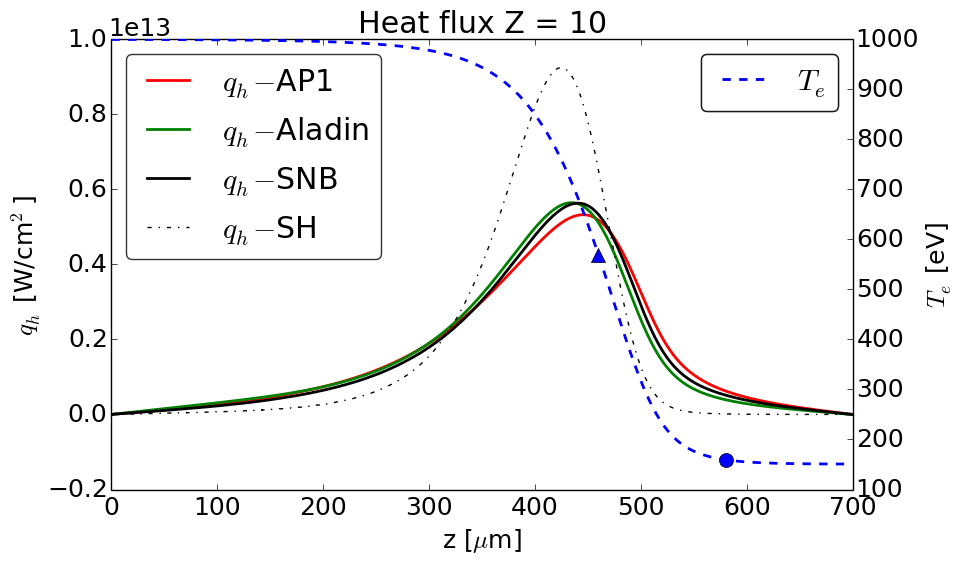
\includegraphics[width=\figscale\textwidth]{../VFPdata/C7_Aladin_case3_heatflux.png} \\
      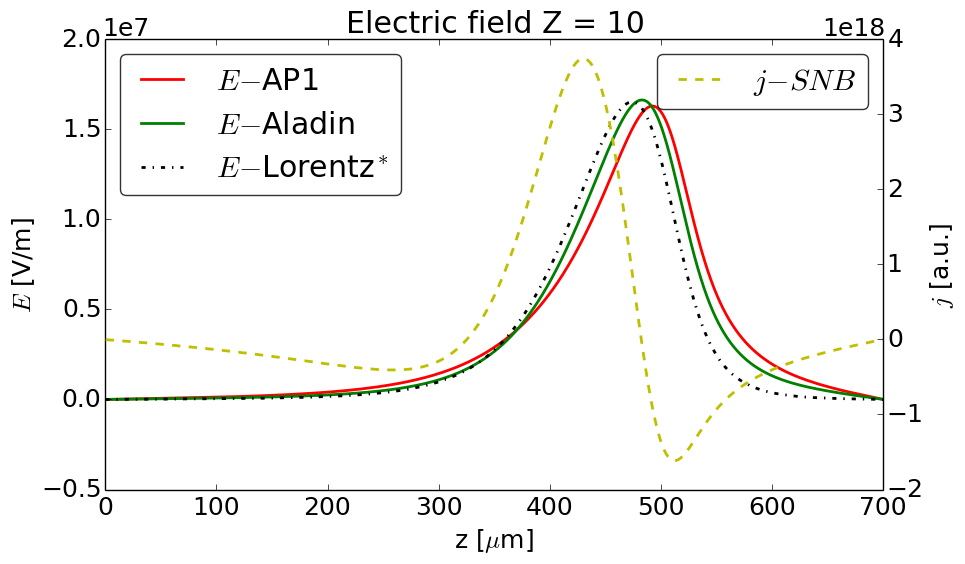
\includegraphics[width=\figscale\textwidth]{../VFPdata/C7_Aladin_case3_Efield.png} \\
      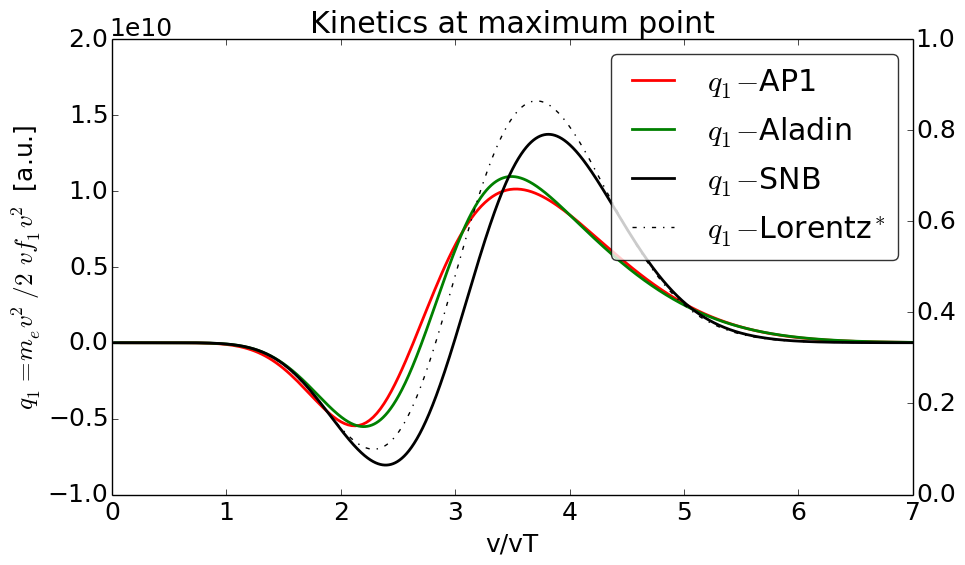
\includegraphics[width=\figscale\textwidth]{../VFPdata/C7_Aladin_case3_kinetics.png} \\
      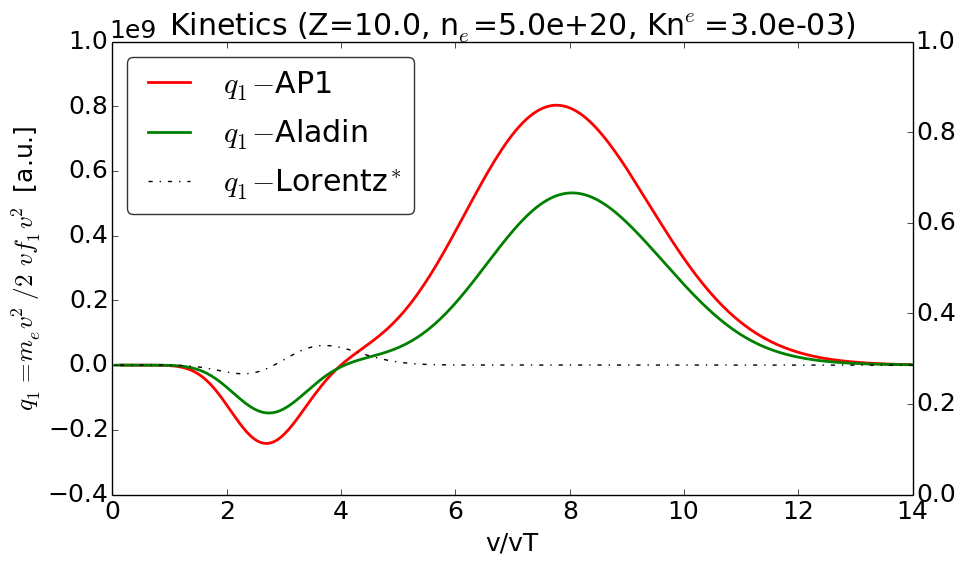
\includegraphics[width=\figscale\textwidth]{../VFPdata/C7_Aladin_case3_nonlocal_kinetics.png}  
    \end{tabular}
  \caption{  
  A~moderate-$\Zbar$ heat-bath problem. The~temperature profile evolved 
  up to 12 ps by Aladin.
  Top plots show heat flux profiles and electric fields by AP1, Aladin, 
  and SNB. The~resulting current of SNB using explicitly the~local electric 
  field $\E_L$ is also shown. Botom plots show a~kinetic detail of
  the~anisotropic part of EDF (its flux velocity moment) at two different 
  spatial points by AP1 and SNB compared to Aladin. 
  %Snapshot 12 ps. Top: correct steady solution of heat flux.  
  %Middle: correct comparison to kinetic profiles at point 460 $\mu$m 
  %by Aladin. 
  %Velocity limit 3.3 $\vth$ at temperature 569.2 eV.
  %Bottom: correct comparison to kinetic profiles at point 580 $\mu$m 
  %by Aladin. Velocity limit 13.1 $\vth$ at temperature 159.4 eV.
  %TODO Fig reordered so change description, E field and current now in Z=10. 
  }
  \label{fig:C7_Aladin_case3}
  \end{center} 
\end{figure}

%Aladin and Impact simulations showed an evolution of the heat flow
%from the local (due to initialising as a Maxwellian) to the
%nonlocal, with a reduced peak, over an initial transient
%phase (over which the temperature ramp flattened somewhat). 
%The transient phase was considered over when the
%ratio of the VFP heat flow to the expected local heat
%flow stopped decreasing. After the transient phase this
%ratio begins to slowly increase as the thermal conduction flattens 
%the temperature ramp and the ratio of the scalelength to mfp increases 
%(i.e. the thermal transport slowly becomes more local). 

The~total computational box size is 700 $\mu$m.
%in the~case of Aladin and Impact and 1000 $\mu$m in the~case of Calder.
We performed Aladin, Impact, and Calder simulations showing an~evolution of
temperature starting from the~initial profile \eqref{eq:T_init}. 
Due to the~initial distribution function being approximated by a~Maxwellian,
the~first phase of the~simulation exhibits a~transient behavior of the~heat
flux. After several ps the~distribution adjusts to its asymptotic form
and the~heat flux profiles can be compared. 
We then take the temperature profiles from Aladin/Impact/Calder and compare 
with AP1 and SNB models which calculate a~stationary heat flow
for a~given temperature profile. 
For all heat-bath simulations the electron density, Coulomb logarithm and 
ionisation were kept constant and uniform.
The~Coulomb logarithm was held fixed throughout, $\lnc = 7.09$.

We show AP1 results for two ionization states, namely $\Zbar = 1$ and 
$\Zbar = 10$ 
in \figref{fig:C7_AladinCalder_case5} and \figref{fig:C7_Aladin_case3}, 
respectively, corresponding to a~moderate nonlocality 
(Kn$^e \sim 10^{-2}$) leading to a~roughly 40 $\%$ inhibition compared 
to the~local SH heat flux maximum. The~original temperature profile steepness
$s = 1/50 \mu$m.
It is preferable to use 
$\text{Kn}^e = \frac{\mfpe(\vth)}{\sqrt{\Zbar + 1}L_{T_e}}$ instead of
 $\text{Kn} = \frac{\mfpei(\vth)}{L_{T_e}}$, 
because $\sqrt{\Zbar + 1}$ provides 
a~better scaling of nonlocality with respect
to ionization \cite{LMV_1983_7}, i.e. the~flux inhibition and Kn$^e$ are
kept approximately the~same when varying $\Zbar$ in 
\figref{fig:C7_AladinCalder_case5} and \figref{fig:C7_Aladin_case3}.
In addition to the~heat flux profiles, we also show the~distribution function 
details related to the~approximate point of the~heat flux maximum (460 $\mu$m) 
and to the~point of the~nonlocal preheat effect (580 $\mu$m) in the~form of
the~flux moment of EDFs anisotropic part \eqref{eq:q1}.
The~nonlocal preheat effect shows a~very good agreement with 
previous results published in \cite{Sherlock_PoP2017}.

The~top left plot of \figref{fig:C7_AladinCalder_case5} shows heat flux 
profiles computed by Aladin, AP1, and SNB corresponding to the~temperature 
$\Te$ profile computed by Aladin and the~top right plot of 
\figref{fig:C7_AladinCalder_case5} shows heat flux profiles computed by Calder, 
AP1, and SNB corresponding to the~temperature $\Te$ profile computed by Calder.
Both kinetic simulations by Aladin and Calder evolved up to 20 ps for 
$\Zbar = 1$. 
The~anisotropic part of EDF, in particular, the~heat flux velocity moment $q_1$, 
at the~heat flux maximum (triangle point) and at~the~nonlocal preheat region 
(circle point) computed by AP1 and SNB for the~temperature profiles by 
Aladin and Calder, can be used as a~detailed comparison of four conceptually
different models: the~full anisotropy form \eqref{eq:LFP_model} of 
the~FP collision operator (Calder); the~isotropic form 
\eqref{eq:C0_collision_operator} of the~FP collision operator (Aladin);
the~simplified linear form \eqref{eq:AWBS_model} of the~FP collision operator
(AWBS in AP1); 
the~nonlocal electron transport model \eqref{eq:SNB_model} (SNB). 
Excellent match of $q_1$ can be seen between 
AP1 and Calder at the~both spatial points. On the~other hand, 
the~AP1 profiles of EDF provide a~reasonable match to Aladin too, however,
one observes a~deviation
%, especially in the~middle plot, 
which resembles to the~low $\Zbar$ trend shown in \figref{fig:q1s_summary}, 
where AP1 corresponds to AWBS and Aladin to BGK curves. To summarize,
various FP-like codes are compared in detail, in particular collisional PIC 
for the first time, and all show a~very good match. 
Furthermore, the~effect of the~anisotropy in the~collision model, 
captured by AP1 and neglected by Aladin and Impact, proves to be important
in the~low-$\Zbar$ plasma. 

In the~case $\Zbar = 10$, we show heat flux profiles
computed by Aladin, AP1, and SNB corresponding to the~temperature $\Te$
profile computed by Aladin up to 12 ps 
in the~top plot of \figref{fig:C7_Aladin_case3}. 
Corresponding profiles of 
a~self-consistently calculated electric fields by Aladin and AP1 
(using the~nonlocal Ohm's law) are shown in the~higher middle plot.
Also the~local theory based electric field $\E_L$ used by SNB is shown.
EDF at the~point of the~approximate heat flux maximum (triangle) of
the~temperature profile is shown in the~lower middle plot, 
where a~very precise match between AP1 and Aladin can be observed, 
and $q_1$ at the~preheat point (circle) of the~temperature profile is shown 
in the~bottom plot. In the~latter case AP1 shows a~very similar properties 
as Aladin with a~difference in magnitude corresponding to a~higher 
heat flux computed by AP1 at this point. 

SNB shows very good results of the~heat flux profile in all three cases, 
i.e. compared to Aladin and Calder in \figref{fig:C7_AladinCalder_case5} 
and to Aladin in \figref{fig:C7_Aladin_case3}. 
However, one can observe that the~EDF kinetic solution of SNB provides 
only a~qualitative image with respect to the~reference green line solution. 
This is illustrated for example in
\figref{fig:C7_Aladin_case3}, where the~kinetics at preheat point plot 
reveals an~insufficient electric field treatment (no return current). 
The~kinetics at maximum point plot shows that the~solution SNB solution
approaches closely the~local Lorentz$^*$ solution and that 
significantly recedes from the~reference fully kinetic solution (green line).
%at the~approximate heat flux maximum
%point in all three cases of $\Zbar$. 
These~discrepancies can be attributed to the~use of an~inconsistent 
electric field in the~case of SNB which uses $\E_L$. An~electric field 
comparison is shown in \figref{fig:C7_Aladin_case3}, where it is shown that 
the~local electric field treatment $\E_L$ used in SNB fails 
in the~preheat region and consequently leads to 
a~significant violation of the~plasma quasi-neutrality,
i.e. a~non-zero current, where one can observe an~uncontrolled stream of 
electrons in the~preheat and also an~overestimation of negative return current
around the~heat flux maximum.

The~AP1 model equations \eqref{eq:AP1f0}, \eqref{eq:AP1f1}, 
and \eqref{eq:AmpereKinetic} in general show a~very good performance 
in all three cases when compared to the~fully kinetic results 
(green line) by Aladin and Calder, which can be assigned 
to the~AWBS collision operator and the~consistent 
treatment of $\E$ via nonlocal Ohm's law \eqref{eq:NonlocalOhm} in
 \eqref{eq:AmpereKinetic} (no $\B$ field in 1D).

In addition, the~Knudsen number Kn$^e$ has been varied among the~simulation 
runs in order to address a~broad range of nonlocality of 
the~electron transport corresponding 
to the~laser-heated plasma conditions, i.e. Kn$^e \in (0.0001, 1)$. 
The~variation of Kn$^e$ arises from the~variation
of the~uniform electron density $n_e \in (10^{19}, 10^{23})$ cm$^{-3}$ or 
the~length scale given by the~slope of the~temperature profile 
$s \in (1/2500, 1/25) \mu$m. Results showing the~heat flux maximum 
of an~extensive set of simulations of
varying Kn$^e$ is shown in \figref{fig:Kn_results}.
 \begin{figure}[htb]
  \begin{center}
    \begin{tabular}{c}
      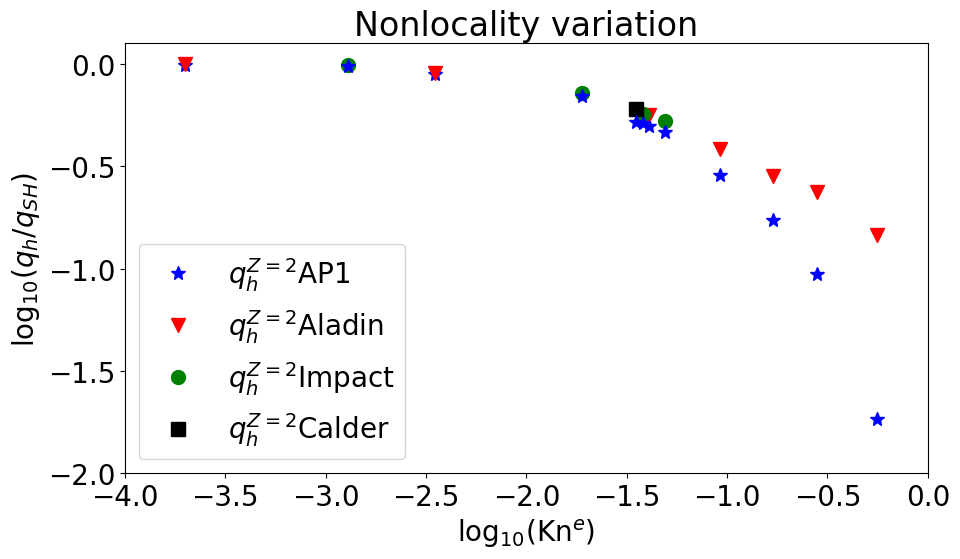
\includegraphics[width=\figscale\textwidth]{Kn_results.png}
    \end{tabular}
  \caption{  
  The~heat-flux inhibition compared to the~local SH theory along varying
  nonlocality (Kn$^e$) in the~heat bath problem. AP1 compares well to 
  the~full kinetic simulations by Aladin, Impact, and Calder, up to 
  Kn$^e \sim 10^{-1}$. For higher nonlocality \textit{decelerating} 
  AP1 departs significanlty from the~reference solutions because of
  the~electric field limiting in accordance with the~velocity limit in 
  \tabref{tab:vlim}. 
  %Simulation results for the case $Z=2$ computed by AP1/Aladin/Impact/Calder.
  %Every point corresponds to the maximum heat flux in a "tanh" temperature 
  %simulation, which can be characterized by Kn. The range of 
  %$\log_{10}(\text{Kn})\in (0, -4)$ can be expressed as equivalent 
  %to the~electron density approximate range n$_e \in (1e19, 3.5e22)$ of 
  %the~50 $\mu$m slope tanh case. In the case of Kn = 0.56, 
  %$q_{Aladin} / q_{AP1}\approx 7.9$.
  }
  \label{fig:Kn_results}
  \end{center} 
\end{figure}
When analyzing the~simulation results shown in \figref{fig:Kn_results}, 
we observed that 
the~maximum of $q_1$ at the~maximum point tends to decrease with increasing 
Kn$^e$ and that the~interval of electron velocities important for 
the~heat transport always belongs to $3 \vth < \vmag <4 \vth$ for an~example
refer to the~kinetics at maximum point in \figref{fig:C7_AladinCalder_case5} 
and \figref{fig:C7_Aladin_case3}. 
%We have also found 
%an~important observation related to the~electron-electron collisions.
According to simulations,
the~stopping force in \eqref{eq:AP1f0} and \eqref{eq:AP1f1} is dominated by
the~electric field for electrons with velocity above the~velocity limit
\begin{equation}
  \vmag_{lim} = \sqrt{\frac{\sqrt{3}\Gamma\me}{2\qe}\frac{n_e}{|\E|}}
  ,
  \label{eq:v_limit}
\end{equation}
and this limit drops 
down significantly with increasing Knudsen number as can be seen 
in \tabref{tab:vlim}. 
As a~consequence, the~electrons responsible for the~heat flux
($3 \vth < \vmag <4 \vth$) are preferably affected by the~electric field
rather than by collisions when Kn$^{e} > 10^{-1}$. According to 
\tabref{tab:vlim} collsions dominate stopping for $\vmag < 3.1 \vth$ 
when Kn$^e = 10^{-1}$ and even a~much lower value $\vmag < 1.8 \vth$ 
when Kn$^e = 1.0$. This explains the~unsatisfactory results of 
the~\textit{decelerating} AP1
model for high Kn$^e$ shown in \figref{fig:Kn_results}. 
Notably, the~AP1 limited electric field effect (described in 
\appref{app:AP1limit}) leads to a~steep increase of error with respect 
to VFP code Aladin for Kn$^e > 10^{-1}$. 
For example $\vmag_{lim}\sim 4.3\vth$ for the~maximum point EDF in 
\figref{fig:C7_AladinCalder_case5}.

Unfortunately, \eqref{eq:v_limit} also leads to a~limitation of 
the~\textit{decelerating} AP1 model, where the~strength of the~stopping/accelerating effect due to the~electric field on electrons must always 
be kept less than the~e-e collision friciton. Details are shown 
in \appref{app:AP1limit}.

\begin{table}
\begin{center}
  \begin{tabular}{c|ccccc}
    \hline\hline\\
    %Kn$^e$ & $10^{-4}$ & $10^{-3}$ & $10^{-2}$ & $10^{-1}$ & $1$ \\\\
    Kn$^e$ & $\,\,10^{-4}\,\,$ & $\,\,10^{-3}\,\,$ & $\,\,10^{-2}\,\,$ & $\,\,10^{-1}\,\,$ & $\,\,1\,\,$ \\\\
    \hline\\
    $\vmag_{lim} / \vth$ & 70.8 & 22.4 & 7.3 & 3.1 & 1.8\\\\
    \hline\hline
  \end{tabular}
  \caption{
  Scan over varying nonlocality (Kn$^e$) showing the~limit of 
  the~collision friction dominance over the~deceleration of electrons 
  due to the~electric field force. The~electric field effect is dominant
  for electrons with higher velocity than $\vmag_{lim}$ defined in 
  \eqref{eq:v_limit}. Kn$^e$ and $\vth$ are evaluated from the~same 
  plasma profiles.
  %$\sqrt{3}\vmag\frac{\me}{2\qe}\nue > |\E|$.
  }
\label{tab:vlim}
\end{center}
\end{table}

%Yet another observation can be made when analysing the~anisotropic term $q_1$ 
%in \figref{fig:C7_AladinCalder_case5} and \figref{fig:C7_Aladin_case3}. 
%When comparing the~kinetics at maximum and 
%preheat points, both velocity maxima of the~EDF correspond to approximately 
%same electron velocity. This means that the~electrons responsible for 
%the~flux in the~preheat region are those flux dominating electrons 
%from the~maximum point. This provides an~important information
%about the~microscopic motion of electrons on the~nonlocal spatial scale, i.e. 
%a~quantification how far the~fast electrons from the~heat flux maximum 
%are transported before being slowed down significantly. 
%Notice that different reference temperatures and $\vth$ are used 
%in the~maximum and preheat plots, 
%e.g. $\Te = 622$~eV and $\vmag_{q_1^{max}} = 3.24~\vth = 3.39\times10^9$~cm/s 
%at the~maximum point and $\Te = 192$~eV and 
%$\vmag_{q_1^{max}} = 5.95~\vth = 3.46\times10^9$~cm/s at the~preheat point
%in \figref{fig:C7_AladinCalder_case5}.

\begin{comment} % Simulations setup.
In every run of AP1 we used 250~velocity groups in order to avoid
numerical errors in modeling of the~electron kinetics. However, a~smaller 
number of groups, e.g. 50, provides a~very similar results 
(an~error around 10$\%$ in the~heat flux). 
\end{comment} % Simulations setup.

\subsection{Hohlraum problem}
Additionally to the~steep temperature gradients, the~laser-heated plasma 
experiments also involve steep density gradients and variation in ionization,
which are dominant effects in multi-material hohlraums
at the interface between the helium gas-fill and 
the ablated high $\Zbar$ plasma.

In~\cite{Brodrick_PoP2017}, a~kinetic simulation of laser pulse interaction 
with a gas filled hohlraum was presented. 
Plasma profiles provided by a~HYDRA simulation in 1D
geometry of a~laser-heated gadolinium hohlraum containing a~helium 
gas at time of 20 ns were used as input for the~Impact 
\cite{Kingham_JCP2004} VFP code.  
For simplicity, the Coulomb logarithm was treated as a
constant $\lnc_{ei}$ = $\lnc_{ee}$ = 2.1484. In reality, in the~low-density 
corona $\lnc$ reaches 8, which, however, does not affect the~heat flux profile 
significantly. 
%Plasma profiles at 20 nanoseconds of the~HYDRA simulation 
%were used (after spline smoothing) as the~initial conditions for 
%the~IMPACT run (in planar geometry).
\figref{fig:Gd_VFP_10ps_heatflux} shows the~electron temperature $\Te$ 
evolved during 10 ps by Impact and the~electron density $\ed$ profile
%and ionization $\Zbar$ profiles. 
Along with plasma profiles the~heat flux profiles
of AP1, Impact, and SNB are also shown. 
%\textit{Kn profile will be probably added}. 

\begin{figure}[htb]
  \begin{center}
    \begin{tabular}{c}
      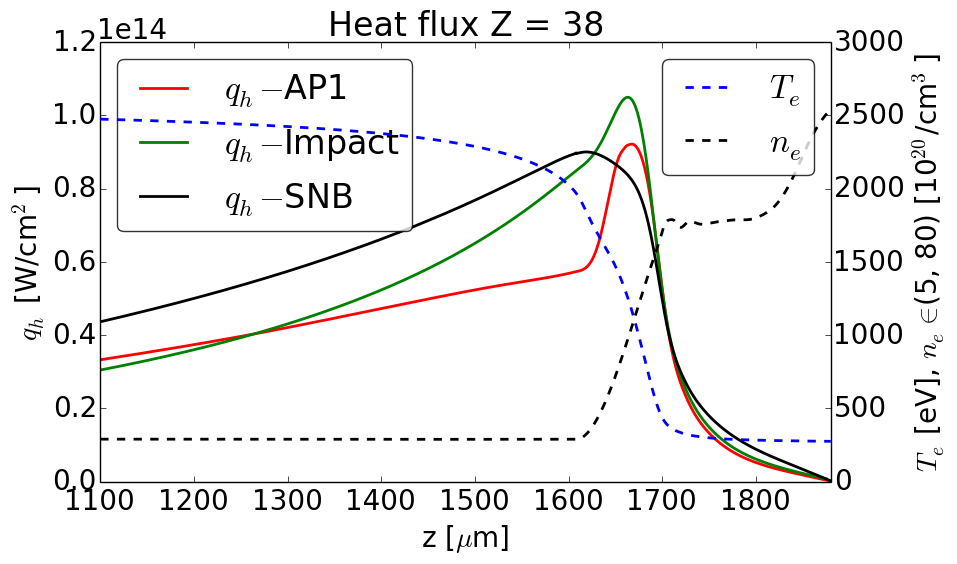
\includegraphics[width=\figscale\textwidth]{../VFPdata/C7_GdHohlraum_heatflux.png}
	  %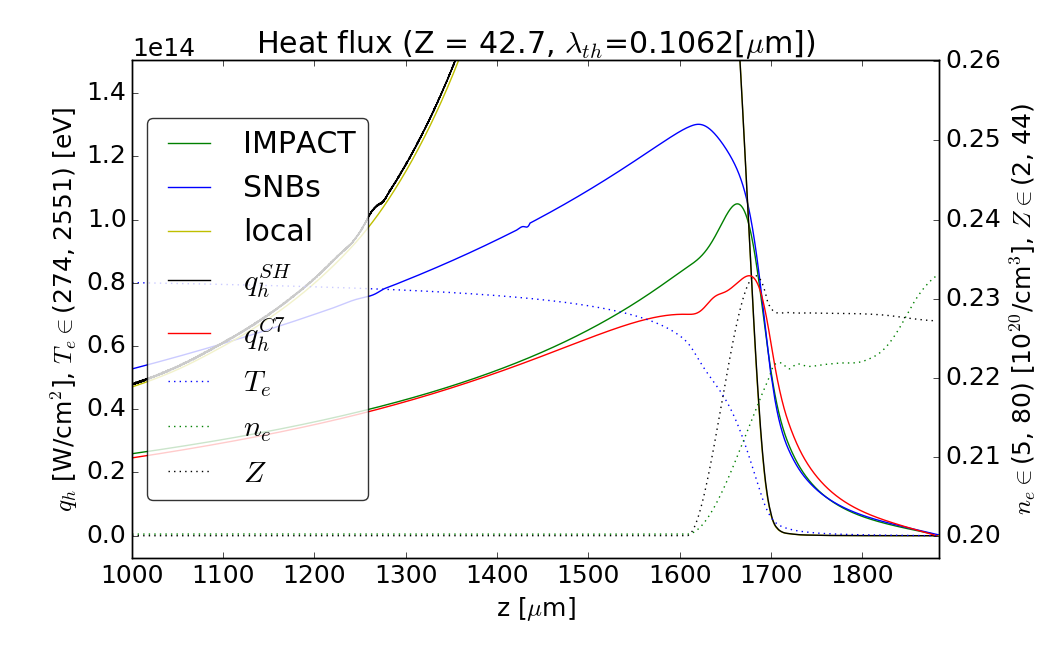
\includegraphics[width=\figscale\textwidth]{../VFPdata/GD_Hohlraum/fluxes_10ps.png} 
    \end{tabular}
  \caption{
  Heat flux profiles by AP1, Impact and SNB along 
  the~electron temperature $\Te$ and electron density $\ed$
  profiles in a~laser-heated gadolinium hohlraum 
  with a~helium gas-fill.
  }
  \label{fig:Gd_VFP_10ps_heatflux}
  \end{center} 
\end{figure}

One can observe a~very good
match between AP1 and Impact computations in the~preheat region.
It is worth mentioning that in the~surroundings of the~heat flux maximum 
($\sim 1662~\mu$m) the~profiles of all plasma variables 
exhibit steep gradients 
with a change from $T_e$ = 2.5 keV, $n_e$ = 5$\times$10$^{20}$ cm$^{−3}$, 
$\Zbar$ = 2 to $T_e$ = 0.3 keV, $n_e$ = 6$\times$10$^{21}$ cm$^{−3}$ , 
$\Zbar$ = 44 across approximately 100 $\mu$m 
(between 1600~$\mu$m and 1700~$\mu$m), starting at the~helium-gadolinium 
interface.  
In this region, we can see a~qualitative match between AP1 and Impact 
providing a~same sign of the~heat flux divergence, however,
the~electric field limitation explained in 
\appref{app:AP1limit} leads to a~stronger drop of 
the~\textit{decelerating} AP1 heat flux on the~material 
interface, which then closely aligns to the~Impact heat flux in the~corona. 
On the~other hand, 
SNB overestimates significantly the~heat flux in the~lower density part 
of plasma up to the~point of the~heat flux maximum given by Impact 
(green line in \figref{fig:Gd_VFP_10ps_heatflux}). More 
importantly, SNB shows the~opposite sign of the~heat flux divergence compared to Impact
(and AP1) in the~steep gradients region close to the~material interface. 
In the~preheat region SNB performs 
very well. Nevertheless, it is important to stress that 
SNB required only 25 velocity groups compared to 250 velocity groups used by
Impact and AP1 for this ICF relevant plasma conditions, thus making it a~very
efficient modeling approach though its description of kinetics is rather
qualitative.
%We also attribute this to the~lack of proper action of the~electric field 
%(the~directional effect) in the~SNB approach.

%

\section{Conclusions}
\label{sec:Conclusions}

\begin{itemize}
  \item The~most important point is that we introduce a~collision operator, 
    which is coherent with the full FP, i.e. no extra dependence on $\Zbar$.
  \item Touch pros/contras of linearized FP in Aladin and Impact vs AWBS
  \item Raise discussion about what is the weakest point of AP1 for high Kns: 
    the~velocity limit or phenomenological Maxwellization?
  \item Summarize useful outcomes related to plasma physics as 
    the~tendency of the~velocity maximum in $q_1$ with respect to $\Zbar$ and
	Kn$^e$.
  \item Emphasize the~good results of Aladin (compared to Impact) and also
    outstanding results of Calder while being PIC. 
\end{itemize}


\begin{acknowledgments}
\end{acknowledgments}

\appendix
\section{Background of the local diffusive regime theory}
\label{app:DiffusiveKinetics}

The~left hand side of \eqref{eq:1D_kinetic_equation} acts on 
\eqref{eq:f_approximation} as
\begin{multline}
  \mu\left(\pdv{\tilde{\ft}}{z} 
  + \frac{\qe\Ez}{\me\vmag}\pdv{\tilde{\ft}}{\vmag}\right) 
  + \frac{\qe\Ez}{\me}\frac{1-\mu^2}{\vmag^2}\pdv{\tilde{\ft}}{\mu} = \\
  \mu\left(\pdv{\ft^0}{z} + \frac{\qe\Ez}{\me\vmag}\pdv{\ft^0}{\vmag}\right) 
  + \frac{\qe\Ez}{\me\vmag^2} \ft^1 + O(\mu^2) .
  \label{app_eq:LHS_kinetic_equation}
\end{multline}
The~action on \eqref{eq:f_approximation} of the~BGK operator 
\eqref{eq:BGK_model_1D} as used in \eqref{eq:1D_kinetic_equation} reads
\begin{eqnarray}
  \frac{1}{\vmag}C_{BGK}(\tilde{\ft})
  &=&
  \frac{\tilde{\ft} - \fM}{\mfpe}
  + \frac{1}{2}\left(\frac{\Zbar}{\mfpe} + \frac{1}{\mfpe}\right)
  \pdv{}{\mu}(1 - \mu^2)\pdv{\tilde{\ft}}{\mu} ,\nonumber\\
  &=&  \frac{\ft^0 - \fM}{\mfpe}
  - \mu \frac{\Zbar}{\mfpe}\ft^1 .
  \label{app_eq:BGK_model_1D}
\end{eqnarray}
Consequently, if the~isotropic and anisotropic parts of 
\eqref{app_eq:LHS_kinetic_equation} and \eqref{app_eq:BGK_model_1D} are 
compared, one finds the~following equations 
\begin{eqnarray}
  \ft^0 &=& \fM + \frac{\mfpe\qe\Ez}{\me\vmag^2}f^1 ,
  \label{app_eq:BGK_f0} \\
  \ft^1 &=& - \frac{\mfpe}{\Zbar}
  \left( \pdv{\ft^0}{z} + \frac{\qe\Ez}{\me\vmag}\pdv{\ft^0}{\vmag} \right) . 
  \label{app_eq:BGK_f1}
\end{eqnarray}
It is valid to assume that $\ft^0 = \fM$ from \eqref{app_eq:BGK_f0}. Then,
\begin{equation}
  \ft^1_{BGK} = - \frac{\mfpe}{\Zbar}
  \left( \pdv{\fM}{z} + \frac{\qe\Ez}{\me\vmag}\pdv{\fM}{\vmag} \right) . 
  \label{app_eq:BGK_f1_fM}
\end{equation}
The~\textit{quasi-neutrality} constraint, corresponding to a~zero current 
imposed by the~electric field reads
\begin{equation}
\vect{j} \equiv \qe \int \vv \tilde{\ft} \, \dI\vv = \vect{0} .
\end{equation}
In the~case of the BGK EDF, in particular its~anisotropic part 
\eqref{app_eq:BGK_f1_fM}, the~zero current condition takes the~form
\begin{equation}
  2\pi\int_{-1}^{1} \int_{\vmag} \vmag \mu^2 \ft^1_{BGK}\, \dI\vmag\dI\mu = 0 ,
  \nonumber
\end{equation}
which leads to the~electric field (same as the~classical Lorentz electric field
$\E_L$ \cite{Lorentz_1905})
\begin{equation}
  \Ez = \frac{\me\vth^2}{\qe}\left(\frac{1}{L_{n_e}} 
  + \frac{5}{2}\frac{1}{L_{T_e}} \right) .
  \label{app_eq:BGK_Efield}
\end{equation}
It is worth mentioning, that the~deviation of $\ft^0$ from $\fM$ in 
\eqref{app_eq:BGK_f0} can be written as $\left(\frac{\mfpe}{L_{n_e}} 
  + \frac{5}{2}\frac{\mfpe}{L_{T_e}} \right)\frac{\vth^2}{\vmag^2}f^1$,
where naturally arises the~Knudsen number 
$Kn = \frac{\mfpe}{L_{n_e}} + \frac{5}{2}\frac{\mfpe}{L_{T_e}}$ comprising
both contributions of electron density and temperature gradients, and that 
a~multiplication of the~electron-electron collision contribution can be 
multiplied by a~constant in \eqref{app_eq:BGK_model_1D} without changing 
the~resulting form of the~local anisotropic term \eqref{app_eq:BGK_f1},
and consequently the~current and heat flux. This constant will be labeled $r$
as introduced in \cite{Brodrick_PoP2017} and the~BGK operator 
\eqref{eq:BGK_model_1D} can be written as 
$r \nue(\tilde{\ft} - \fM) + \frac{\nuei + r \nue}{2}
  \pdv{}{\mu}(1 - \mu^2)\pdv{\tilde{\ft}}{\mu}$. 

In the~case of the~AWBS operator \eqref{eq:AWBS_model} used in 
\eqref{eq:1D_kinetic_equation}, its action on \eqref{eq:f_approximation} reads
\begin{eqnarray}
  \frac{1}{\vmag}C_{AWBS}(\tilde{\ft})
  &=& 
  \frac{\vmag\zeta}{\mfpe} \pdv{}{\vmag}\left(\tilde{\ft} - \fM\right) 
  \nonumber \\
  && + \frac{1}{2}\left(\frac{\Zbar}{\mfpe} + \frac{\zeta}{\mfpe}\right)
  \pdv{}{\mu}(1 - \mu^2)\pdv{\tilde{\ft}}{\mu}  \nonumber \\
  &=& \frac{\vmag\zeta}{\mfpe} \pdv{}{\vmag}\left(\ft^0 - \fM\right) \nonumber \\ 
  &&\, + \mu\left(\frac{\vmag\zeta}{\mfpe} \pdv{\ft^1}{\vmag} 
  - \frac{\Zbar+\zeta}{\mfpe}\ft^1\right) ,
  \label{app_eq:AWBS_model_1D}
\end{eqnarray}
where $\nue^* = \zeta \nue = \frac{\vmag\zeta}{\mfpe}$ with $\zeta$ being a~scaling
parameter of the~standard e-e collision frequency. Its purpose is to
match AWBS heat flux to results obtained by Spitzer and Harm 
\cite{SpitzerHarm_PR1953} obtained for any $\Zbar$. 
\secref{sec:FPDiffusiveRegime} shows that this match can be found with 
a~constant $\zeta=0.5$.

One finds the~following equations if the~isotropic and anisotropic parts of 
\eqref{app_eq:LHS_kinetic_equation} and \eqref{app_eq:AWBS_model_1D} are 
compared 
\begin{eqnarray}
  \pdv{}{\vmag}\left( \ft^0 -\fM\right) &=& 
  \frac{\mfpe\qe\Ez}{\zeta\me\vmag^2}\frac{\ft^1}{\vmag} ,
  \label{app_eq:AWBS_f0} \\
  \frac{\vmag\zeta}{\mfpe} \pdv{\ft^1}{\vmag} 
  - \frac{\Zbar+\zeta}{\mfpe}\ft^1 &=&
  \pdv{\ft^0}{z} + \frac{\qe\Ez}{\me\vmag}\pdv{\ft^0}{\vmag} .
  \label{app_eq:AWBS_f1} 
  %\\  
  %\frac{\vmag}{\Zbar}\pdv{f^1}{\vmag} + \frac{4}{\Zbar}f^1 
  %- \frac{\Zbar + 1}{\Zbar} f^1 &=&
  %\pdv{f^0}{z} + \frac{\tilde{E}_z}{\vmag}\pdv{f^0}{\vmag}
  %\nonumber
\end{eqnarray}
If we assume that $\pdv{\ft^0}{\vmag} = \pdv{\fM}{\vmag}$, i.e. $\ft^0 = \fM$,
the~anisotropic part of the~AWBS operator is governed by the~equation
\begin{equation}
  \pdv{\ft^1_{AWBS}}{\vmag} 
  - \frac{\Zbar+\zeta}{\vmag\zeta}\ft^1_{AWBS} =
  \frac{\mfpe}{\vmag\zeta} 
  \left(\pdv{\fM}{z} + \frac{\qe\Ez}{\me\vmag}\pdv{\fM}{\vmag}\right) .
  \label{app_eq:AWBS_f1_fM}
\end{equation}
Even though it is not straightforward, the~electric field in 
\eqref{app_eq:AWBS_f1_fM} (solved numerically) providing a~zero current 
exactly matches \eqref{app_eq:BGK_Efield}. Consequently, the~deviation of
$\pdv{\ft^0}{\vmag}$ from $\pdv{\fM}{\vmag}$ in 
\eqref{app_eq:AWBS_f0} can be written as 
$Kn\frac{\vth^2}{\zeta\vmag^2}\frac{f^1}{\vmag}$.

Finally, it should be stressed, that the~concept of locality expressed as 
$Kn\ll1$ is crucial for our \textit{local diffusive regime} analysis, 
because it provides sufficient Maxwellization, i.e.  \eqref{app_eq:BGK_f0} and
\eqref{app_eq:AWBS_f0}, and correspondingly, \eqref{app_eq:BGK_f1_fM} 
and \eqref{app_eq:AWBS_f1_fM} are valid models.

\section{AP1 electric field limit}
\label{app:AP1limit}

Interestingly, we have encountered a~very specific property of the~AP1 model
with respect to the~electric field magnitude. The~easiest way how to 
demonstrate this is to write the~model equations \eqref{eq:AP1f0} and 
\eqref{eq:AP1f1} in 1D (z-axis). Then, due to its linear nature, it is easy 
to eliminate one of the~partial derivatives with respect to $\vmag$, i.e. 
$\pdv{\fzero}{\vmag}$ or $\pdv{\fonez}{\vmag}$. 
In the~case of elimination of $\pdv{\fzero}{\vmag}$ 
one obtains the~following equation
\begin{multline}
  %\frac{2}{3\vmag\nue} 
  %\left(\left(\sqrt{3}\vmag\frac{\nue}{2}\right)^2 - \Ez^2\right)  
  \left(\vmag\frac{\nue}{2} - \frac{2\qe^2\Ez^2}{3\me^2\vmag\nue}\right) 
  \pdv{\fonez}{\vmag} 
  =
  \frac{2\qe\Ez}{3\me\nue}\pdv{\fonez}{z}  
  + \frac{4\pi\qe\Ez}{3\me}\pdv{\fM}{\vmag} \\
  + \frac{\vmag}{3}\pdv{\fzero}{z} 
  + \left(\frac{4\qe^2\Ez^2}{3\me^2\vmag^2\nue}
  + \left(\nuei + \frac{\nue}{2}\right) \right)\fonez .
  \label{eq:AP1_model_1D}
\end{multline}
It is convenient to write the~bracket on the~left hand side of 
\eqref{eq:AP1_model_1D} as
$\frac{2}{3\vmag\nue} 
\left(\left(\sqrt{3}\vmag\frac{\nue}{2}\right)^2 
- \frac{\qe^2}{\me^2}\Ez^2\right)$
from where it is clear that the~bracket is negative if 
$\sqrt{3}\vmag\frac{\nue}{2} < \frac{\qe}{\me}|\E|$, 
i.e. there is a~velocity limit for a~given magnitude $|\E|$, 
when the~collisions are no more fully dominant and the~electric field 
introduces a~comparable effect to the~collision friction in 
the~electron transport.

It can be shown, that the~last term on the~right hand side of 
\eqref{eq:AP1_model_1D} is dominant and the~solution behaves as 
\begin{equation}
  \Delta \fone \sim \exp\left(\frac{\frac{4\qe^2\Ez^2}{3\me^2\vmag^2\nue}
  + \left(\nuei + \frac{\nue}{2}\right)}
  {\vmag\frac{\nue}{2} - \frac{2\qe^2\Ez^2}{3\me^2\vmag\nue}}\, 
  \Delta\vmag\right) ,
  \label{eq:f1z_behavior}
\end{equation}
where $\Delta \vmag < 0$ represents a~velocity step of the~implicit Euler
numerical integration of decelerating electrons.
However, \eqref{eq:f1z_behavior} exhibits an~exponential growth 
for velocities above the~friction limit (bracket on the~left hand side of 
\eqref{eq:AP1_model_1D})
\begin{equation}
  \vmag_{lim}  = \sqrt{\frac{\sqrt{3}\Gamma\me}{2\qe}\frac{n_e}{|\E|}} ,
  \label{eq:v_limit}
\end{equation}
which makes the~problem to be ill-posed.

In order to provide a~stable model, we introduce a~reduced electric field
to be acting as the~accelerating force of electrons
\begin{equation}
  |\E_{red}| = \sqrt{3} \vmag\frac{\me}{\qe}\frac{\nue}{2} ,
  \label{eq:Elimit}
\end{equation}
ensuring that the~bracket on the~left hand side of \eqref{eq:AP1_model_1D}
remains positive. We define a~quantity $\eta_{red} = \frac{|\E_{red}|}{|\E|}$.
Then, the~AP1 model \eqref{eq:AP1f0}, \eqref{eq:AP1f1} can be formulated 
as well posed 
\begin{eqnarray}
  \vmag\frac{\nue}{2}\pdv{}{\vmag}\left(\fzero - \fM \right) &=&
  \frac{\vmag}{3}\nabla\cdot\fone + \frac{\qe}{\me}\frac{\E}{3}\cdot
  \nonumber \\
  &&\left(
  \eta_{red}\pdv{\fone}{\vmag} + \frac{2(2-\eta_{red})}{\vmag}\fone\right) , 
  \nonumber \\
  \label{eq:AP1f0_app}\\
  \vmag\frac{\nue}{2}\pdv{\fone}{\vmag}
  - \nuscat\fone &=& 
  \vmag\nabla\fzero + 
  \frac{\qe\eta_{red}}{\me}\E\pdv{\fzero}{\vmag} 
  +\frac{\qe\B}{\me c}\vect{\times} \fone
  ,
  \nonumber \\
  \label{eq:AP1f1_app}
\end{eqnarray}
while introducing the~reduction factor of the~accelerating electric field
and the~compensation of the~electric field effect via its angular term.  

\begin{comment} % delta f0.
Nevertheless, before doing so,
we introduce a~slightly different approximation to the~electron distribution 
function as
\begin{equation}
  \tilde{f} = \frac{4\pi \fM + \dafzero}{4\pi} + \frac{3}{4\pi}\vn\cdot\fone .
  \label{eq:P1_OOE}
\end{equation}
where $\dafzero$ represents the~departure of isotropic part from 
the~Maxwell-Boltzmann equilibrium distribution $\fM$. 
%which we keep 
%intentionally in the~distribution function approximation.
Then, the~stable AP1 model reads
\begin{eqnarray}
  \vmag \frac{\nue}{2}\pdv{\dafzero}{\vmag} &=&
  \vmag\nabla\cdot\fone 
  + \frac{\qe}{\me}\E\cdot\left(\omega_{red} \pdv{\fone}{\vmag} 
  + \frac{2}{\vmag}\fone\right) , 
  \label{eq:AP1f0_stable}\\
  \vmag\frac{\nue}{2}\pdv{\fone}{\vmag} 
  &=& \tnuscat\fone 
  + \frac{\vmag}{3}\nabla\left(4\pi\fM + \dafzero\right)
  \nonumber \\
  && 
  + \frac{\qe\E}{3\me}\left(4\pi \pdv{\fM}{\vmag} 
  + \omega_{red} \pdv{\dafzero}{\vmag} 
  \right) ,
  \label{eq:AP1f1_stable}
\end{eqnarray}
where $\tnuscat = \nuei + \nuscat^E + \frac{\nue}{2}$.

The~reason for keeping $\fM$ in the~distribution function approximation
\eqref{eq:P1_OOE} can be seen in the~last term on the~right hand side of 
\eqref{eq:AP1f1_stable}, which provides the~effect of electric field on
directional quantities as current or heat flux. In principle, the~explicit use
of $\fM$ ensures the~proper effect of $\E$ if $\dafzero \ll \fM$, i.e.
no matter what the~reduction $\omega_{red}$ is. Apart from its stability,
it also exhibits much better convergence of the~electric field, which is now
given by the~zero current condition of \eqref{eq:AP1f1_stable} as
\begin{equation}
  \E =
  \frac{\intv \left(\frac{\nue}{2\tnuscat}\vmag^2\pdv{\fone}{\vmag}
  - \frac{\vmag^2}{3\tnuscat}
  \nabla\left(4\pi\fM + \dafzero\right)\right) \vmag^2\, \dI\vmag}
  {\frac{\qe}{\me}\intv \frac{\vmag}
  {3\tnuscat}
  \left(4\pi\pdv{\fM}{\vmag} + \omega_{red} \pdv{\dafzero}{\vmag}\right)
  \vmag^2\, \dI\vmag} .
  \label{eq:AP1_Efield_stable}
\end{equation}
\end{comment} % delta f0.

\begin{comment} % CALDER kinetics.
\section{Calder kinetics}
\label{app:CalderKinetics}
and is written (it would be better to write Eq. (2) in its conservative forme and its non relativistic kernel U):
\begin{widetext}
\begin{eqnarray}
&&\frac{\partial f_\alpha}{\partial t}+\mathbf{v}\cdot\nabla_{\mathbf{x}}f_\alpha+q_\alpha\left(\mathbf{E}+\mathbf{v}\vect{\times}\mathbf{B}\right)\nabla_{\mathbf{p}}f_\alpha=C_{LBB}(f_\alpha,f_\alpha)+\sum_\beta C_{LBB}(f_\alpha,f_\beta),\\
&&C_{LBB}(f_\alpha,f_\beta)=-\frac{\partial}{\partial \mathbf{p}}\cdot\frac{\Gamma_{\alpha\beta}}{2}\left[\int \mathbf{U}(\mathbf{p},\mathbf{p}^\prime)\cdot(f_\alpha\nabla_{\mathbf{p}^\prime}f_\beta^\prime-f_\beta^\prime\nabla_{\mathbf{p}}f_\alpha)\right]d^3\mathbf{p}^\prime,\\
&&\mathbf{U}(\mathbf{p},\mathbf{p}^\prime)=\frac{r^2/\gamma\gamma^\prime}{(r^2-1)^{3/2}}\left[(r^2-1)\mathbf{I}-\mathbf{p}\otimes\mathbf{p}-\mathbf{p}^\prime\otimes\mathbf{p}^\prime+r(\mathbf{p}\otimes\mathbf{p}^\prime+\mathbf{p}^\prime\otimes\mathbf{p})\right],
\end{eqnarray}
\end{widetext}
with $\gamma=\sqrt{1+\mathbf{p}^2}$, $\gamma^\prime=\sqrt{1+\mathbf{p}^{\prime 2}}$ and $r=\gamma\gamma^\prime-\mathbf{p}\cdot\mathbf{p}^\prime$. The momemtum $\mathbf{p}_\alpha$ ($\mathbf{p}_\beta$) is normalized to $m_\alpha c$ (resp. $m_\beta c$). Obviously, this collision operator tends to Eq. (2) in the non-relativistic limit.
\end{comment} % CALDER kinetics.



\bibliographystyle{elsarticle-num}
\bibliography{NTH}

%% Authors are advised to submit their bibtex database files. They are
%% requested to list a bibtex style file in the manuscript if they do
%% not want to use elsarticle-num.bst.

\clearpage

\end{document}

%% Old stuff goes to appendix 
\appendix
\section{The~Fokker-Planck equation}
\label{sed:FP}
%Use equation Hu (1, 2, 3) in text, (10), which puts together (4, 5, 7),
%and	write definitions (11, 12) using (5, 7, 13) and after define (6, 8)
%and to close write (31) from Tzoufras.
\begin{equation}
  \pdv{\ft}{t} + \vv\cdot\gx \ft + (\tE + \vv\times\tB) \cdot\gv \ft =
  - \gv \cdot \sum_{\pb}\vect{S}_c^{\tob} ,
  \nonumber
\end{equation}
where the~collision flux of test particles (labeled $\ft$) colliding on field
particles (labeled $\fb$) takes the~Landau-Fokker-Planck (LFP) form
\begin{equation}
  \vect{S}_c^{\tob} = \Gamma^{\tob}\int \gv\gv\vs \cdot \left[ 
  \ft(\vv)\frac{m_\pt}{m_\pb}\gvb \fb(\vvb) - \fb(\vvb)\gv \ft(\vv)
  \right]\, \dI\vvb , \nonumber 
  %&=& \vect{F}^{\tob}(\fb)\, \ft - \matr{D}^{\tob}(\fb)\cdot\gv\ft ,
  \nonumber
\end{equation} 
where $\Gamma^{\tob} = \frac{4\pi\Zbar_\pt^2\Zbar_\pb^2 q^4 \lnc}{m_\pt^2}$, $\vs = \vv - \vvb$, and 
$\frac{\MI}{\vsmag} - \frac{\vs\vs}{\vsmag^3} = \gv\gv\vs$ was used.
%The friction and diffusion coefficients of collision flux are then defined as
%\begin{eqnarray}
%  \vect{F}^{\tob}(\fb) &=& \frac{1}{m_\pb} 
%  \int \gv\gv\vs\cdot\gvb \fb(\vvb)\,\dI\vvb = -\Gamma^{\tob}\gv 
%  \Rh(\vv) ,
%  \nonumber \\
%  \matr{D}^{\tob}(\fb) &=& \frac{1}{m_\pt} 
%  \gv\gv\int \vs \fb(\vvb)\,\dI\vvb = -\Gamma^{\tob}\gv\gv \Rg(\vv) ,
%  \nonumber
%\end{eqnarray}
The~LFP integral collision model can written in the~form introduced by 
Rosenbluth 1957
\begin{equation}
  \left(\pdv{\ft}{t}\right)_{\pb} = - \gv \cdot \vect{S}_c^{\tob} = 
  - \Gamma^{\tob} \left[ \gv\cdot\left(\ft \gv\Rhb\right)
  - \frac{\gv\gv:\left(\ft \gv\gv\Rgb \right)}{2}\right] ,
  \label{eq:FP_Rosenbluth}
\end{equation}
where $\left(\pdv{\ft}{t}\right)_{\pb}$ expresses the~rate of change in 
the~distribution function of test particles $\ft$ due to collisions with
background field particles (distribution function $\fb$) and
where the~complicated nature of collisions is modeled by the~Rosenbluth 
potentials 
\begin{equation}
  \Rhb(\vv) = \frac{m_\pt + m_\pb}{m_\pb}
  \int \frac{\fb(\vvb)}{|\vv - \vvb|}\, \dI\vvb ,
  \quad \Rgb(\vv) = \int \fb(\vvb)|\vv - \vvb|\, \dI\vvb ,
  \nonumber
\end{equation}
which have the following properties
\begin{equation}
  \gv\cdot\gv \Rhb = 
  -4\pi \frac{m_\pt + m_\pb}{m_\pb} \Gamma^{\tob}\fb ,\quad
  \gv\cdot\gv \Rgb = 
  2 \frac{m_\pb}{m_\pt + m_\pb} \Rhb .
  \nonumber
\end{equation}
The~Rosenbluth equation \refeq{eq:FP_Rosenbluth} can be further rewritten
according to $[$Longmire, Conrad L. : Elementary Plasma Physics. Intersci. Pub., 1963$]$ as
\begin{equation}
  \left(\pdv{\ft}{t}\right)_c = \sum_{\pb} \Gamma^{\tob} 
  \left[ 4\pi \frac{m_{\pt}}{m_\pb} \fb \ft 
  + \frac{m_\pb - m_\pt}{m_\pt + m_\pb} \gv\Rhb\cdot\gv \ft 
  + \frac{\gv\gv\Rgb : \gv\gv \ft}{2} \right] ,
  \label{eq:FP_Longmire}
\end{equation}
which was also published in Shkarofsky 1966 and used in Tzoufras 2011.

%\subsection{Spherical harmonics expansion}
%\label{sec:FP_spherical_harmonics}
%Write Hu (14, 15) and full (1) in spherical coordinates. Then explicitly write
%(17, 18, 23, 24, 25). Further define spherical harmonics expansion and 
%from Tzoufras (34, 35, 36, 37).

\subsection{The linearized Fokker-Planck equation for low anisotropy}
\label{sec:FP_linear}
Define the anisotropic perturbation as in Tzoufras and then use the equations
(32, 33) and the harmonic expansions (38, 39, 40) and the most importantly (41)
for one-kind particles. Finally, write explicitly (41) for the case $f_1^0$
and write set of integrals $I, J$ and constants $C_1, .., C_6$,
which will be used to calculate FP equation solution for diffusive conditions.

If we write the~distribution function as its isotropic and anisotropic parts, 
i.e. $\ft = \ft_0 + \delta\ft$ and $\fb = \fb_0 + \delta\fb$, 
then the~linearized LFP operator for low anisotropy of order 
$O(\delta\ft^2, \delta\fb^2)$ reads 
\begin{eqnarray}
  \frac{1}{\Gamma^{\tob}} \left(\pdv{\ft_0}{t}\right)_{\pb} &=&  
  4\pi \frac{m_{\pt}}{m_\pb} \fb_0 \ft_0 
  + \frac{m_\pb - m_\pt}{m_\pt + m_\pb} \gv\Rh(\fb_0)\cdot\gv \ft \nonumber \\ 
  &&+ \frac{\gv\gv\Rg(\fb_0) : \gv\gv \ft_0}{2} ,
  \label{eq:FP_f0} \\ 
  \frac{1}{\Gamma^{\tob}}\left(\pdv{\delta\ft}{t}\right)_{\pb} &=&  
  4\pi \frac{m_{\pt}}{m_\pb} 
  \left(\fb_0\delta\ft + \ft_0\delta\fb\right) \nonumber \\ 
  &&+ \frac{m_\pb - m_\pt}{m_\pt + m_\pb} 
  \left(\gv\Rh(\fb_0)\cdot\gv \delta\ft + \gv\ft_0\cdot\gv\Rh(\delta\fb)\right)
  \nonumber \\ 
  &&+ \frac{\gv\gv\Rg(\fb_0) : \gv\gv \delta\ft}{2} 
  + \gv\gv \ft_0 : \frac{\gv\gv\Rg(\delta\fb)}{2} .
  \label{eq:FP_deltaf} 
\end{eqnarray}

\begin{eqnarray}
  \ft &=& \ft_0 + \sum_{l=1}^\infty\sum_{m=-l}^l \ft^m_l(\vmag) 
  P_l^{|m|}(\cos \theta) \exp^{i m \phi} ,
  \nonumber \\ 
  \fb &=& \fb_0 + \sum_{l=1}^\infty\sum_{m=-l}^l \fb^m_l(\vmag) 
  P_l^{|m|}(\cos \theta) \exp^{i m \phi} ,
  \nonumber
\end{eqnarray}

\begin{eqnarray}
  I_j(\fb_l^m) &=& \frac{4\pi}{\vmag^j} \int_0^\vmag \fb_l^m(u) u^{j+2}
  \, \dI u ,
  \nonumber \\
  J_j(\fb_l^m) &=& \frac{4\pi}{\vmag^j} \int_\vmag^\infty 
  \fb_l^m(u) u^{j+2}\, \dI u ,
  \nonumber
\end{eqnarray}

\begin{equation}
  \frac{1}{\Gamma^{\tob}}\left(\pdv{\ft_0}{t}\right)_{\pb} =
  \frac{1}{3\vmag^2}\pdv{}{\vmag}\left[\frac{3 m_\pt}{m_\pb} 
  \ft_0 I_0(\fb_0) + \vmag \left( I_2(\fb_0) + J_{-1}(\fb_0)\right)
  \pdv{\ft_0}{\vmag} \right] ,
  \nonumber
\end{equation}

\begin{multline}
  \frac{1}{\Gamma^{\tob}}\left(\pdv{\ft_l^m}{t}\right)_{\pb} = 
  4\pi\frac{m_\pt}{m_\pb} \left[\fb_0 \ft_l^m + \ft_0 \fb_l^m \right] 
  \\
  + \frac{m_\pt-m_\pb}{m_\pb \vmag^2} \left[ \pdv{\ft_0}{\vmag}
  \left(\frac{l+1}{2 l+1} I_l(\fb_l^m) 
  - \frac{l}{2 l +1} J_{-1-l}(\fb_l^m)\right) 
  + I_0(\fb_0)\pdv{\ft_l^m}{\vmag}\right] 
  \\
  + \frac{I_2(\fb_0) + J_{-1}(\fb_0)}{3\vmag}
  \frac{\partial^2 \ft_l^m}{\partial\vmag^2} + 
  \frac{-I_2(\fb_0) + 2 J_{-1}(\fb_0) + 3 I_0(\fb_0)}{3\vmag^2}
  \pdv{\ft_l^m}{\vmag}
  \\
  - \frac{l(l+1)}{2}
  \frac{-I_2(\fb_0) + 2 J_{-1}(\fb_0) + 3 I_0(\fb_0)}{3\vmag^3} \ft_l^m 
  \\
  \frac{1}{2 \vmag} \frac{\partial^2 \ft_0}{\partial\vmag^2}
  \left[C_1 I_{l+2}(\fb_l^m) + C_1 J_{-l-1}(\fb_l^m) + C_2 I_l(\fb_l^m) 
  + C_2 J_{1-l}(\fb_l^m) \right]
  \\
  \frac{1}{\vmag^2} \pdv{\ft_0}{\vmag}
  \left[C_3 I_{l+2}(\fb_l^m) + C_4 J_{1-l}(\fb_l^m) + C_5 J_{-l-1}(\fb_l^m) 
  + C_6 I_l(\fb_l^m) \right]
  \label{eq:FP_flm}
\end{multline}
\begin{eqnarray}
  C_1 = \frac{(l+1)(l+2)}{(2l+1)(2l+3)}, 
  C_2 = -\frac{(l-1)l}{(2l +1)(2l-1)},
  C_3 = -\frac{l(l+1)/2 + (l+1)}{(2l+1)(2l+3)},
  \nonumber \\
  C_4 = \frac{l(l+1)/2 - l}{(2l+1)(2l-1)},
  C_5 = \frac{(l+2) - l(l+1)/2}{(2l+1)(2l+3)}, 
  C_6 = \frac{l(l+1)/2 + (l-1)}{(2l+1)(2l-1)}, 
  \nonumber
\end{eqnarray}

In the~case of massive background particles $m_\pt / m_\pb << 1$ in equilibrium
and comparable temperatures $T_\pb\approx T_\pb$, 
i.e. slow-non-moving background, 
the~isotropic distribution function can be approximated by 
$\fb_0^{slow} = n_{slow} \delta(\vmag) / (4\pi\vmag^2)$, 
and since all integrals 
$I_j(\fb_0^{slow}), J_j(\fb_0^{slow})$ vanish except 
$I_0(\fb_0^{slow}) = n_{slow}$, equation \refeq{eq:FP_flm} reduces to 
\begin{equation}
  \frac{1}{\Gamma^{\pt/slow}}\left(\pdv{\ft_l^m}{t}\right)_{slow} = 
  - \frac{l(l+1)}{2}
  \frac{n_{slow}}{\vmag^3} \ft_l^m 
  \label{eq:FP_flm_slow}
\end{equation} 
where $n_{slow}$ is the~density of slow massive particles. Consequently, 
the~effect of collisions on slow massive particles leads to scattering but no
change in velocity, i.e. energy, of test particles.

\subsection{Plasma Fokker-Planck equation in diffusive regime}
\begin{equation}
  \left(\pdv{\ft_0}{t}\right)_{e} =
  \frac{\Gamma^{e/e}}{3\vmag^2}\pdv{}{\vmag}\left[3 
  \ft_0 I_0(\ft_0) + \vmag \left( I_2(\ft_0) + J_{-1}(\ft_0)\right)
  \pdv{\ft_0}{\vmag} \right] ,
  \nonumber
\end{equation}

\begin{multline}
  \left(\pdv{\ft_l^m}{t}\right)_{e} = \Gamma^{e/e} \Bigg[
  8\pi \ft_0 \ft_l^m  
  - \frac{l(l+1)}{2}
  \frac{3 I_0(\ft_0) - I_2(\ft_0) + 2 J_{-1}(\ft_0)}{3\vmag^3} \ft_l^m
  \\
  + \frac{I_2(\ft_0) + J_{-1}(\ft_0)}{3\vmag}
  \frac{\partial^2 \ft_l^m}{\partial\vmag^2} + 
  \frac{3 I_0(\ft_0) - I_2(\ft_0) + 2 J_{-1}(\ft_0)}{3\vmag^2}
  \pdv{\ft_l^m}{\vmag} 
  \\
  + \frac{1}{2 \vmag} \frac{\partial^2 \ft_0}{\partial\vmag^2}
  \left[C_1 I_{l+2}(\ft_l^m) + C_1 J_{-l-1}(\ft_l^m) + C_2 I_l(\ft_l^m) 
  + C_2 J_{1-l}(\ft_l^m) \right]
  \\
  + \frac{1}{\vmag^2} \pdv{\ft_0}{\vmag}
  \left[C_3 I_{l+2}(\ft_l^m) + C_4 J_{1-l}(\ft_l^m) + C_5 J_{-l-1}(\ft_l^m) 
  + C_6 I_l(\ft_l^m) \right] \Bigg]
\end{multline}

\begin{equation}
  C_1 = \frac{2}{5}, 
  C_2 = 0,
  C_3 = -\frac{1}{5},
  C_4 = 0,
  C_5 = \frac{2}{15}, 
  C_6 = \frac{1}{3}, 
  \nonumber
\end{equation}

%\begin{multline}
%  \frac{1}{\Gamma^{e/e}}\left(\pdv{\ft_1}{t}\right)_{e} = 
%  8\pi \ft_0 \ft_1  
%  - \frac{-I_2(\ft_0) + 2 J_{-1}(\ft_0) + 3 I_0(\ft_0)}{3\vmag^3} \ft_1
%  \\
%  + \frac{I_2(\ft_0) + J_{-1}(\ft_0)}{3\vmag}
%  \frac{\partial^2 \ft_1}{\partial\vmag^2} + 
%  \frac{-I_2(\ft_0) + 2 J_{-1}(\ft_0) + 3 I_0(\ft_0)}{3\vmag^2}
%  \pdv{\ft_1}{\vmag} 
%  \\
%  + \frac{1}{5 \vmag} \frac{\partial^2 \ft_0}{\partial\vmag^2}
%  \left[I_{3}(\ft_1) + J_{-2}(\ft_1)\right]
%  + \frac{1}{15 \vmag^2} \pdv{\ft_0}{\vmag}
%  \left[5 I_1(\ft_1) - 3 I_{3}(\ft_1) + 2 J_{-2}(\ft_1) 
%  \right]
%\end{multline}

\begin{multline}
  \left(\pdv{\ft_1}{t}\right)_{e+i} = \Gamma^{e/e}\Bigg[
  8\pi \ft_0 \ft_1  
  - \left[\frac{3 I_0(\ft_0) - I_2(\ft_0) + 2 J_{-1}(\ft_0)}{3\vmag^3} +
  \frac{\Zbar n_e}{\vmag^3}\right] \ft_1
  \\
  +   \frac{3 I_0(\ft_0) -I_2(\ft_0) + 2 J_{-1}(\ft_0)}{3\vmag^2}
  \pdv{\ft_1}{\vmag}
  + \frac{I_2(\ft_0) + J_{-1}(\ft_0)}{3\vmag}
  \frac{\partial^2 \ft_1}{\partial\vmag^2} 
  \\
  + \frac{1}{5 \vmag} \frac{\partial^2 \ft_0}{\partial\vmag^2}
  \left[I_{3}(\ft_1) + J_{-2}(\ft_1)\right]
  + \frac{1}{15 \vmag^2} \pdv{\ft_0}{\vmag}
  \left[5 I_1(\ft_1) - 3 I_{3}(\ft_1) + 2 J_{-2}(\ft_1) 
  \right] \Bigg]
\end{multline}

\begin{equation}
  \ft \approx \fM + \cos(\theta) \mfpei(\vmag) 
  \left[\frac{\vmag^2}{2\vth^2} - 4 + D\left(\vmag\right) \right] \fM ,
  \nonumber
\end{equation}

\begin{multline}
  \vmag\pdv{\fM}{z} - \frac{\vmag\tEz}{\vth^2}\fM = \Gamma^{e/e}\Bigg[
  8\pi \fM \ft_1  
  - \frac{3 I_0(\fM) - I_2(\fM) + 2 J_{-1}(\fM) + 3 \Zbar n_e}{3\vmag^3} \ft_1
  \\
  +   \frac{3 I_0(\fM) -I_2(\fM) + 2 J_{-1}(\fM)}{3\vmag^2}
  \pdv{\ft_1}{\vmag}
  + \frac{I_2(\fM) + J_{-1}(\fM)}{3\vmag}
  \frac{\partial^2 \ft_1}{\partial\vmag^2} 
  \\
  + \frac{\fM}{15 \vmag\vth^2} \left[\frac{3\vmag^2}{\vth^2}
  \left[I_{3}(\ft_1) + J_{-2}(\ft_1)\right]
  - 5 \left[I_1(\ft_1) + J_{-2}(\ft_1)\right]
  \right] \Bigg]
  \nonumber
\end{multline}

\begin{multline} 
  \left[\frac{I_2(\fM) + J_{-1}(\fM)}{3\vmag}\right]
  \frac{\partial^2 \ft_1}{\partial\vmag^2}
  + \left[\frac{3 I_0(\fM) -I_2(\fM) + 2 J_{-1}(\fM)}{3\vmag^2}\right]
  \pdv{\ft_1}{\vmag}
  \\ 
  + \left[8\pi \fM  - \frac{3 I_0(\fM) - I_2(\fM) + 2 J_{-1}(\fM)}{3\vmag^3}
  - \frac{\Zbar n_e}{\vmag^3} \right] \ft_1 =
  \\
  \frac{1}{\Gamma^{e/e}}
  \left[\vmag\pdv{\fM}{z} - \frac{\vmag\tEz}{\vth^2}\fM\right]
  - \frac{\fM}{15 \vmag\vth^2} \left[\frac{3\vmag^2}{\vth^2}
  \left[I_{3}(\ft_1) + J_{-2}(\ft_1)\right]
  - 5 \left[I_1(\ft_1) + J_{-2}(\ft_1)\right]
  \right]
  \label{eq:FP_f1_diffusive}
\end{multline}

\begin{equation} 
  a \frac{\partial^2 \ft_1}{\partial\vmag^2} + b \pdv{\ft_1}{\vmag} + c \ft_1 
  = d
  \nonumber
\end{equation}

Integration of \refeq{eq:FP_f1_diffusive} from $\infty \rightarrow 0$
\begin{eqnarray}
  a^{n-0.5} \frac{df^n - df^{n-1}}{ - \Delta \vmag} &=& b^{n-0.5} df^{n-1} 
  + c^{n-0.5} \ft_1^{n-1} + d^{n-0.5} ,
  \nonumber \\
  \frac{\ft_1^n - \ft_1^{n-1}}{- \Delta \vmag} &=& df^{n-1} ,
  \nonumber
\end{eqnarray}
\begin{eqnarray}
  \left(\frac{a^{n-0.5}}{\Delta \vmag} - b^{n-0.5}\right) df^{n-1} 
  - c^{n-0.5} \ft_1^{n-1}&=&  d^{n-0.5} + \frac{a^{n-0.5}}{\Delta \vmag} df^n,
  \nonumber \\
  - df^{n-1} + \frac{1}{\Delta \vmag} \ft_1^{n-1} &=&  
  \frac{1}{\Delta \vmag} \ft_1^n ,
  \nonumber
\end{eqnarray}

\begin{equation}
  \begin{bmatrix}
    - c^{n-0.5}  &
	\frac{a^{n-0.5}}{\Delta \vmag} - b^{n-0.5}
    \\
	\frac{c^{n-0.5}}{\Delta \vmag} & -c^{n-0.5} 
  \end{bmatrix}
  \begin{bmatrix}
    \ft_1^{n-1} \\
    df^{n-1}
  \end{bmatrix}
  =  
  \begin{bmatrix}
    d^{n-0.5} + \frac{a^{n-0.5}}{\Delta \vmag} df^n \\
    \frac{c^{n-0.5}}{\Delta \vmag} \ft_1^n
  \end{bmatrix}   ,
  \nonumber
\end{equation}

\begin{multline}
  \begin{bmatrix}
    - c^{n-0.5}  &
	\frac{a^{n-0.5}}{\Delta \vmag} - b^{n-0.5} 
    \\
	0 & 
	\frac{1}{\Delta \vmag}
	\left(\frac{a^{n-0.5}}{\Delta \vmag} - b^{n-0.5}\right) - c^{n-0.5} 
  \end{bmatrix}
  \begin{bmatrix}
    \ft_1^{n-1} \\
    df^{n-1}
  \end{bmatrix}
  =  \\
  \begin{bmatrix}
    d^{n-0.5} + \frac{a^{n-0.5}}{\Delta \vmag} df^n \\
    \frac{1}{\Delta \vmag} \left(c^{n-0.5}\ft_1^n + 
	d^{n-0.5} + \frac{a^{n-0.5}}{\Delta \vmag} df^n \right) 
  \end{bmatrix}   ,
  \nonumber
\end{multline}

\begin{eqnarray}
  a^n &=& \frac{I^n_2(\fM) + J^n_{-1}(\fM)}{3\vmag^n} ,
  \nonumber \\
  b^n &=& \frac{3 I^n_0(\fM) - I^n_2(\fM) + 2 J^n_{-1}(\fM)}{3{\vmag^n}^2} ,
  \nonumber \\
  c^n &=& 8\pi \fM^n  - \frac{3 I^n_0(\fM) - I^n_2(\fM) + 2 J^n_{-1}(\fM)}
  {3{\vmag^n}^3} - \frac{\Zbar n_e}{{\vmag^n}^3},
  \nonumber \\
  d^n &=& \frac{1}{\Gamma^{e/e}}
  \left[\vmag^n\pdv{\fM^n}{z} - \frac{\vmag^n\tEz}{\vth^2}\fM^n\right]
  \nonumber \\
  &&- \frac{\fM^n}{15 \vmag^n\vth^2} \left[\frac{3{\vmag^n}^2}{\vth^2}
  \left[I^n_{3}(\ft_1) + J^n_{-2}(\ft_1)\right]
  - 5 \left[I^n_1(\ft_1) + J^n_{-2}(\ft_1)\right] \right]
  \nonumber
\end{eqnarray}

\begin{eqnarray}
  I^n_0(g) = 4\pi \int_0^{\vmag^n} g(u) u^{2}
  \, \dI u ,\quad
  I^n_1(g) = \frac{4\pi}{\vmag^n} \int_0^{\vmag^n} g(u) u^{3}
  \, \dI u ,
  \nonumber \\
  I^n_2(g) = \frac{4\pi}{{\vmag^n}^2} \int_0^{\vmag^n} g(u) u^{4}
  \, \dI u ,\quad 
  I^n_3(g) = \frac{4\pi}{{\vmag^n}^3} \int_0^{\vmag^n} g(u) u^{5}
  \, \dI u ,
  \nonumber \\
  J^n_{-1}(g) = 4\pi\vmag^n \int_{\vmag^n}^\infty 
  g(u) u\, \dI u ,\quad
  J^n_{-2}(g) = 4\pi{\vmag^n}^2 \int_{\vmag^n}^\infty 
  g(u) \, \dI u ,
  \nonumber
\end{eqnarray}

\section{AWBS-P1 modeling of laser heated plasmas}\label{sec:OOE_AWBSP1}
\subsection{Model equations}
The~AWBS electron transport equation reads
\begin{multline}
  \vmag\vn\cdot\nabla f + \tE\cdot\vn \pdv{f}{\vmag} 
  + \frac{\tE\cdot\vect{e}_\phi 
  - \vmag\tB\cdot\vect{e}_\theta}{\vmag}\pdv{f}{\phi}
  =
  \vmag \nue \pdv{}{\vmag}\left(f - f_M\right) 
  + (\nuei + \nue) (\fzero - f) ,
  \nonumber \label{eq:AWBS_model}
\end{multline}
where $\nue$ is the~electron-electron collision frequency, 
$\nuei$ is the~electron-ion collision frequency, and $\nuei = \Zbar \nue$.

In order to eliminate the~dimensions of the~above transport problem 
the~first-two-moment model based on approximation 
\begin{equation}
  f = \frac{\fzero}{4\pi} + \frac{3}{4\pi}\vn\cdot\fone , 
  \nonumber \label{eq:OOE_P1approximation}
\end{equation}
can be adopted and reads
\begin{eqnarray}
  \nue\vmag\pdv{}{\vmag}\left(\fzero - \tfM \right) &=&
  \vmag\nabla\cdot\fone + \tE\cdot
  \pdv{\fone}{\vmag} + \frac{2}{\vmag}\tE\cdot\fone , 
  \nonumber \label{eq:OOE_P1f0}\\
  \nue\vmag\pdv{}{\vmag}\fone - \nutot\fone &=& 
  \vmag\nabla\cdot\left(\MA\fzero\right) + 
  \tE\cdot\pdv{\left(\MA\fzero\right)}{\vmag} + \tB\times\fone ,
  \nonumber \label{eq:OOE_P1f1}
\end{eqnarray}
where $\tfM = 4\pi \fM$ and the~closure matrix takes the~form
\begin{equation}
  \MA = \frac{1}{3}\MI .
  \nonumber \label{eq:OOE_P1closure}
\end{equation}

Since in the~laser heated plasmas the~Knudsen number 
Kn$ = \frac{\vth}{\nu_t(\vth) L} \in (0, 1)$, i.e. the~collisionality in 
the~kinetics of electrons plays always an~important effect for thermal-like 
particles, the~electron distribution 
function can be treated as out-of-equilibrium approximation 
\begin{equation}
  f = \fM + \daf ,
  \label{eq:OOE_outofeq}
\end{equation}  
where the~consequent AWBS model reads
\begin{multline}
  \vmag\vn\cdot\nabla (\fM + \daf) + \tE\cdot\vn \pdv{\fM}{\vmag} 
  + \tE\cdot\vn \pdv{\daf}{\vmag} 
  + \frac{\tE\cdot\vect{e}_\phi 
  - \vmag\tB\cdot\vect{e}_\theta}{\vmag}\pdv{\daf}{\phi}
  = \\
  \vmag \nue \pdv{\daf}{\vmag} 
  + (\nuei + \nue) (\fzero - \fM - \daf) ,
  \label{eq:OOE_AWBS_model}
\end{multline}
or its P1 approximation equivalent
\begin{equation}
  f = \frac{4\pi \fM + \dafzero}{4\pi} + \frac{3}{4\pi}\vn\cdot\fone .
  \label{eq:OOE_P1outofeq}
\end{equation}
where the~moment model reads
\begin{eqnarray}
  \nue\vmag\pdv{\dafzero}{\vmag} &=&
  \vmag\nabla\cdot\fone + \tE\cdot
  \pdv{\fone}{\vmag} + \frac{2}{\vmag}\tE\cdot\fone , 
  \label{eq:OOE_P1f0}\\
  \nue\vmag\pdv{\fone}{\vmag} - \nutot\fone &=& 
  \frac{\vmag}{3}\nabla\dafzero + 
  \frac{\tE}{3}\pdv{\dafzero}{\vmag} + \tB\times\fone 
  \nonumber \\
  & & + \frac{\vmag}{3}\nabla\tfM + \frac{\tE}{3}\pdv{\tfM}{\vmag} .
  \label{eq:OOE_P1f1}
\end{eqnarray}

\subsection{A~consistent treatment of $\tE$ field}
\label{sec:OOE_E_treatment}
The~plasma conditions providing an~appropriate electric field
are the~best expressed via the~definition of current
\begin{equation}
  \vect{q}_c(\vect{x}) = \intv
  \vmag\fone(\vect{x}) \vmag^2\, \dI\vmag , 
  \nonumber 
\end{equation}
which can be directly expressed from \refeq{eq:OOE_P1f1} as
\begin{equation}
  %\frac{\vect{j}}{\qe} = 
  \vect{q}_c =
  \intv \left(\frac{\nue\vmag^2}{\nutot}\pdv{\fone}{\vmag}
  - \frac{\vmag^2}{3\nutot}\nabla\left(\tfM + \dafzero\right) - 
  \frac{\vmag}{3\nutot}\pdv{\left(\tfM + \dafzero\right)}{\vmag}\tE
  \right) \vmag^2\, \dI\vmag ,
  \label{eq:OOE_P1current}
\end{equation}
where the $\B$ field and $\E$ field scattering effect (angular) have been 
omitted.  

Then, the~current can be easily evaluated based on
\begin{eqnarray}
  a_0(\vect{x}) &=& \intv\frac{\vmag}{3 \nutot} \pdv{\left(\tfM + \dafzero\right)}{\vmag}(\vect{x})
  \vmag^2\, \dI\vmag , \nonumber \\
  \vect{b}_{0}(\vect{x}) &=& \intv\left(  
  \frac{\vmag^2}{3 \nutot}\nabla\left(\tfM(\vect{x}) + \dafzero(\vect{x})\right)
  - \frac{\nue\vmag^2}{\nutot}\pdv{\fone}{\vmag}(\vect{x})
  \right)\vmag^2\, \dI\vmag , \nonumber 
\end{eqnarray}
%Alors, treat $a_0, \vect{b}_{0}, \vect{b}_1$ as grid functions, 
%where it is obvious to express 
%$\pdv{a_0}{\vmag}, \pdv{\vect{b}_{0}}{\vmag}, \pdv{\vect{b}_1}{\vmag}$ in 
%ImplicitSolve().
as the~following generalization of the~Ohm's law
\begin{equation}
  \vect{q}_c(\vect{x}) 
  = -\vect{b}_{0}(\vect{x}) 
  - a_{0}(\vect{x})\tE(\vect{x}) ,
  \nonumber \label{eq:OOE_HOFcurrent}
\end{equation}
where one needs the~actual distribution function $f$ values.

%\begin{equation}
%  \tE(\vect{x}) = -\frac{\vect{b}_{0}(\vect{x})}{a_{0}(\vect{x})} 
%  - \frac{\vect{q}_c(\vect{x})}{a_{0}(\vect{x})}
%   + \frac{\vect{b}_{1}(\vect{x})}{a_{0}(\vect{x})}\times\tB(\vect{x}) ,
%  \nonumber \label{eq:OOE_HOFcurrent}
%\end{equation}

It is straightforward to find the~\textit{zero current} formula for 
the~electric field
\begin{equation}
  \tE(\vect{x}) = -\frac{\vect{b}_{0}(\vect{x})}{a_{0}(\vect{x})} .
  \label{eq:OOE_E_j0}
\end{equation}

\subsection{AWBS model analysis}
\label{sec:OOE_AWBS_model_analysis}
The~AWBS transport equation can be written as the~following
\begin{multline}
  \left(\vmag \nue - \tE\cdot\vn\right)\pdv{\daf}{\vmag} 
  %+ \frac{\tE\cdot\vect{e}_\phi 
  %- \vmag\tB\cdot\vect{e}_\theta}{\vmag}\pdv{f}{\phi}
  =
  \vmag\vn\cdot\nabla (\fM + \daf) + \tE\cdot\vn\pdv{\fM}{\vmag} 
  + (\nuei + \nue) (\fM + \daf - \fzero) ,
  \label{eq:OOE_AWBS_model_analysis}
\end{multline}
in order to stress the~effect of force applied to electrons, i.e. the~effect
of friction described by $\nue$ and the~Lorentz force effect via $\tE$, 
and their competition.

The~same reformulation can be written for the~moment AWBS model
\begin{eqnarray}
  \pdv{\dafzero}{\vmag} &=&
  \frac{1}{\nue\vmag}\left(\vmag\nabla\cdot\fone + \tE\cdot
  \pdv{\fone}{\vmag}\right) , 
  \nonumber\\
  \nue\vmag\pdv{\fone}{\vmag} - \nutot\fone &=& 
  \frac{\vmag}{3}\nabla\dafzero + 
  \frac{\tE}{3}\pdv{\dafzero}{\vmag}
  + \frac{\vmag}{3}\nabla\tfM + \frac{\tE}{3}\pdv{\tfM}{\vmag} ,
  \nonumber
\end{eqnarray}
and it takes the~following form
\begin{equation}
  \left(\nue\vmag\MI - \frac{\tE\tE}{3 \nue\vmag}\right)\cdot
  \pdv{\fone}{\vmag} = 
  \frac{\vmag}{3}\nabla\dafzero + \frac{\tE}{3 \nue}\nabla\cdot\fone
  + \frac{\vmag}{3}\nabla\tfM + \frac{\tE}{3}\pdv{\tfM}{\vmag} 
  + \nutot\fone ,
  \nonumber \label{eq:OOE_P1AWBS_model_analysis}
\end{equation}
which is especially instructive in 1D
\begin{equation}
  \left(\nue\vmag - \frac{\tEz^2}{3 \nue\vmag}\right)
  \pdv{\fonez}{\vmag} = 
  \frac{\vmag}{3}\pdv{\dafzero}{z} + \frac{\tEz}{3 \nue}\pdv{\fonez}{z}
  + \frac{\vmag}{3}\pdv{\tfM}{z} + \frac{\tEz}{3}\pdv{\tfM}{\vmag} 
  + \nutot\fonez ,
  \label{eq:OOE_P1AWBS_model_1Danalysis}
\end{equation}
because it gives a \textit{"reverse-time-like evolution"} condition
\begin{equation}
  \sqrt{3} \nue > \frac{|\tEz|}{\vmag} .
  \label{eq:OOE_reverse_time_condition}
\end{equation}

\begin{equation}
  \pdv{\fonez}{\vmag} = 
  \frac{3 \nue\vmag}{3 (\nue\vmag)^2 - \tEz^2}
  \left(
  \frac{\vmag}{3}\pdv{\dafzero}{z} + \frac{\tEz}{3 \nue}\pdv{\fonez}{z}
  + \frac{\vmag}{3}\pdv{\tfM}{z} + \frac{\tEz}{3}\pdv{\tfM}{\vmag} 
  + \nutot\fonez\right) ,
  \label{eq:OOE_P1AWBS_model_1Danalysis}
\end{equation}
because it gives a \textit{"reverse-time-like evolution"} condition
\begin{equation}
  3(\nue\vmag)^2 - \tEz^2 \neq 0 ,
  \nonumber
\end{equation}
or a~numerical stability formulation
because it gives a \textit{"reverse-time-like evolution"} condition
\begin{equation}
  |3(\nue\vmag)^2 - \tEz^2| > \epsilon .
  \label{eq:OOE_reverse_time_condition}
\end{equation}
which can be obtained from
\begin{equation}
  \left(3(\nue\vmag)^2 - \tEz^2\right)^2 - \epsilon^2 = 0 .
  \label{eq:OOE_reverse_time_condition}
\end{equation}

\subsection{\textit{"Reverse-time-like evolution"} model by splitting}
\label{sec:OOE_stable_splitting}
Full separation of advection and E field
\begin{eqnarray}
  \nue\vmag \pdv{\fone^{\nue}}{\vmag} &=& 
  \frac{\vmag}{3}\nabla\dafzero^{\nue}
  + \frac{\vmag}{3}\nabla\tfM + \nutot\fone^{\nue} ,
  \nonumber \\
  \frac{\tE\tE}{3 \nue\vmag}\cdot
  \pdv{\fone^{\tE}}{\vmag} &=& -\frac{\tE}{3 \nue}\nabla\cdot\fone^{\tE} 
  - \frac{\tE}{3}\pdv{\tfM}{\vmag},
  \nonumber
\end{eqnarray}
or separation of stable "bulk" E field effect and implicit E field effect
\begin{eqnarray}
  \nue\vmag \pdv{\fone^{\nue}}{\vmag} &=& 
  \frac{\vmag}{3}\nabla\dafzero^{\nue}
  + \frac{\vmag}{3}\nabla\tfM + \nutot\fone^{\nue} 
  + \frac{\tE}{3}\pdv{\tfM}{\vmag},
  \nonumber \\
  \frac{\tE\tE}{3 \nue\vmag}\cdot
  \pdv{\fone^{\tE}}{\vmag} &=& -\frac{\tE}{3 \nue}\nabla\cdot\fone^{\tE} ,
  \nonumber
\end{eqnarray}
and the~complete effect of diffusion in velocity space reads
\begin{equation}
  \pdv{\fone}{\vmag} = \pdv{\fone^{\nue}}{\vmag} + \pdv{\fone^{\tE}}{\vmag} ,
  \nonumber
\end{equation}

\begin{comment}
\begin{multline}
  \IV_{\left(\MA \cdot \tE\right)} \cdot
  \left[
  \frac{1}{\vmag} \IM^{0^{-1}}_{(\nue)} \cdot \IV^T_{\left(\tE\right)} \cdot 
  \pdv{\fone}{\vmag} 
  + \IM^{0^{-1}}_{(\nue)} \cdot \left( \ID^T_{\left(\MI\right)} 
  + \frac{2}{\vmag^2}\IV^T_{\left(\tE\right)} \right)\cdot  
  \left(\fone^n 
  + \Delta\vmag\pdv{\fone}{\vmag}\right)\right] = \\
  -\IV_{\left(\MA \cdot \tE\right)} \cdot
  \pdv{\tvfM}{\vmag} .
  \nonumber
\end{multline}
\end{comment}

\subsection{\textit{"Friction"} model}
\label{sec:OOE_stable_splitting}
\newcommand{\nuE}{\nu_{\tE}}
In order to obey \refeq{eq:OOE_reverse_time_condition}, an~additional friction
$\nu_{\tE}$ can be introduced as
\begin{eqnarray}
  |\tE| &=& |\tE^*| + \nuE \vmag  ,
  \nonumber \\
  \nue + \nuE &=& \frac{|\tE^*|}{\vmag} ,
  \nonumber
\end{eqnarray}
which is then applied to perturbation $\dafzero$ as
\begin{eqnarray}
  \left(\nue + \nuE\right) \vmag \pdv{\dafzero}{\vmag} &=&
  \vmag\nabla\cdot\fone + \tE^*\cdot\pdv{\fone}{\vmag} , 
  \nonumber\\
  \left(\nue + \frac{\nuE}{3}\right) \vmag\pdv{\fone}{\vmag} - \nutot\fone &=& 
  \frac{\vmag}{3}\nabla\dafzero + 
  \frac{\tE^*}{3}\pdv{\dafzero}{\vmag}
  + \frac{\vmag}{3}\nabla\tfM + \frac{\tE}{3}\pdv{\tfM}{\vmag} .
  \nonumber
\end{eqnarray}

\begin{comment} % Implicit fully-discrete scheme
\subsection{Implicit fully-discrete scheme}
\label{sec:OOE_impl_fullydiscrete_scheme}
The moment P1 model \refeq{eq:OOE_P1f0}, \refeq{eq:OOE_P1f1} can be written 
in a~semi-discrete form
\begin{eqnarray}
  \IM^0_{(\nue)} \cdot \pdv{\davfzero}{\vmag}  
  &=& 
  \left(\ID^T_{\left(\MI\right)}
  + \frac{2}{\vmag^2}\IV^T_{\left(\tE\right)}\right) \cdot \fone
  + \frac{1}{\vmag}\IV^T_{\left(\tE\right)} \cdot 
  \pdv{\fone}{\vmag} ,  
  \nonumber \label{eq:OOE_semiM1hosf0} \\
  \IM^1_{(\nue)} \cdot \pdv{\fone}{\vmag}  
  &=& 
  - \ID_{\left(\MA\right)}\cdot\davfzero
  + \frac{1}{\vmag}\IV_{\left(\MA \cdot \tE\right)} \cdot
  \pdv{\davfzero}{\vmag}
  + \frac{1}{\vmag}\left(
  \IM^1_{\left( \nutot \right)} + \IB_{\left( \tB \right)}  
  \right) \cdot \fone
  \nonumber\\
  & & - \ID_{\left(\MA\right)}\cdot \tvfM
  + \frac{1}{\vmag}\IV_{\left(\MA \cdot \tE\right)} \cdot
  \pdv{\tvfM}{\vmag} .
  \label{eq:OOE_semiM1hosf1}
\end{eqnarray}
It is convenient to define
\begin{equation}
  \matr{DIVE} = \ID^T_{\left(\MI\right)} 
  + \frac{2}{\vmag^2}\IV^T_{\left(\tE\right)}.
  \nonumber
\end{equation}
The next step goes towards implicit Runge-Kutta method (DIRK).
Then, a~very effective inversion in the~L2 space can be formally performed
\begin{equation}
  \pdv{\davfzero}{\vmag}  
  = \frac{1}{\vmag}
  \IM^{0^{-1}}_{(\nue)} \cdot \IV^T_{\left(\tE\right)} \cdot 
  \pdv{\fone}{\vmag} 
  + \IM^{0^{-1}}_{(\nue)} \cdot \matr{DIVE}\cdot  
  \left(\fone^n 
  + \Delta\vmag\pdv{\fone}{\vmag}\right) .
  \label{eq:OOE_fullP1hosf0}
\end{equation}
The~first moment equation in the DIRK framework reads
\begin{multline}
  \IM^1_{(\nue)} \cdot \pdv{\fone}{\vmag}  
  = \frac{1}{\vmag}\IV_{\left(\MA \cdot \tE\right)} \cdot
  \pdv{\davfzero}{\vmag}
  - \ID_{\left(\MA\right)}\cdot \left(\tvfM^n + \davfzero^n 
  + \Delta\vmag\pdv{\davfzero}{\vmag}\right)\\ 
  + \frac{1}{\vmag}\left(\IB_{\left( \tB \right)} 
  + \IM^1_{\left( \nutot \right)}\right) 
  \cdot \left(\fone^n 
  + \Delta\vmag\pdv{\fone}{\vmag}\right)
  + \frac{1}{\vmag}\IV_{\left(\MA \cdot \tE\right)} \cdot
  \pdv{\tvfM^n}{\vmag} .
  \label{eq:OOE_semiM1hosf1}
\end{multline}
Finally, one can eliminate $\pdv{\davfzero}{\vmag}$, 
which leads to the~final form
\begin{multline}
  \IM^1_{(\nue)} \cdot \pdv{\fone}{\vmag}  
  = 
  \left(\frac{1}{\vmag}\IV_{\left(\MA \cdot \tE\right)}
  - \Delta\vmag \ID_{\left(\MA\right)} \right) \cdot
  \IM^{0^{-1}}_{(\nue)} \cdot 
  \left(\frac{1}{\vmag} \IV^T_{\left(\tE\right)} 
  + \Delta\vmag \matr{DIVE}
  \right)
  \cdot \pdv{\fone}{\vmag}
  \\
  +\frac{\Delta\vmag}{\vmag}\left(\IB_{\left( \tB \right)} 
  + \IM^1_{\left( \nutot \right)}\right) 
  \cdot \pdv{\fone}{\vmag} + 
  \frac{1}{\vmag}\left(\IB_{\left( \tB \right)} 
  + \IM^1_{\left( \nutot \right)}\right) 
  \cdot \fone^n
  + \frac{1}{\vmag}\IV_{\left(\MA \cdot \tE\right)} \cdot
  \pdv{\tvfM^n}{\vmag}
  \\ 
  +\left(\frac{1}{\vmag}\IV_{\left(\MA \cdot \tE\right)}
  - \Delta\vmag \ID_{\left(\MA\right)} \right) \cdot
  \IM^{0^{-1}}_{(\nue)} \cdot \matr{DIVE}\cdot\fone^n 
  - \ID_{\left(\MA\right)}\cdot\left(\tvfM^n + \davfzero^n\right),
  \label{eq:OOE_fullP1hosf1}
\end{multline}
where the~only unknown is $\pdv{\fone}{\vmag}$. Once \refeq{eq:OOE_fullP1hosf1}
is solved the~completion of the~solution 
$[\pdv{\davfzero}{\vmag}, \pdv{\fone}{\vmag}]$ is achieved by evaluating 
\refeq{eq:OOE_fullP1hosf0}.
\cite{Dobrev_Kolev_Rieben-High-order_curvilinear_finite_element_methods_for_Lagrangian_hydrodynamics}
\end{comment} % Implicit fully-discrete scheme

\section{Simulation results}\label{sec:results}
Three cases:
\begin{itemize}
  \item constant $n_e = 5\times10^{20}$ [1/cm$^3$], constant $\Zbar = 4$, 
  $T_e$ temperature profile taken from Impact simulation at 12 ps, see Figure 1
  %\figref{fig:Philippe_VFP_12ps}
  \item $n_e, T_e, \Zbar$ profiles taken from HYDRA simulation of Gadolinium
  hohlraum at 10 ps, see Figure 2 and Figure 3
  %\figref{fig:Gd_VFP_10ps_heatflux} and \figref{fig:Gd_VFP_10ps_kinetics} 
  \item Detail of distribution function under diffusive conditions of hydrogen 
  raising the~question of potentially outstanding properties of AWBS, since
  the uncorrected AWBS result is very close to KIPP full collision operator,
  see Figure 4 (consult Eq. (41) in Tzoufras OSHUN JCP 2011) 
\end{itemize}
\begin{figure}[tbh]
  \begin{center}
    \begin{tabular}{c}
      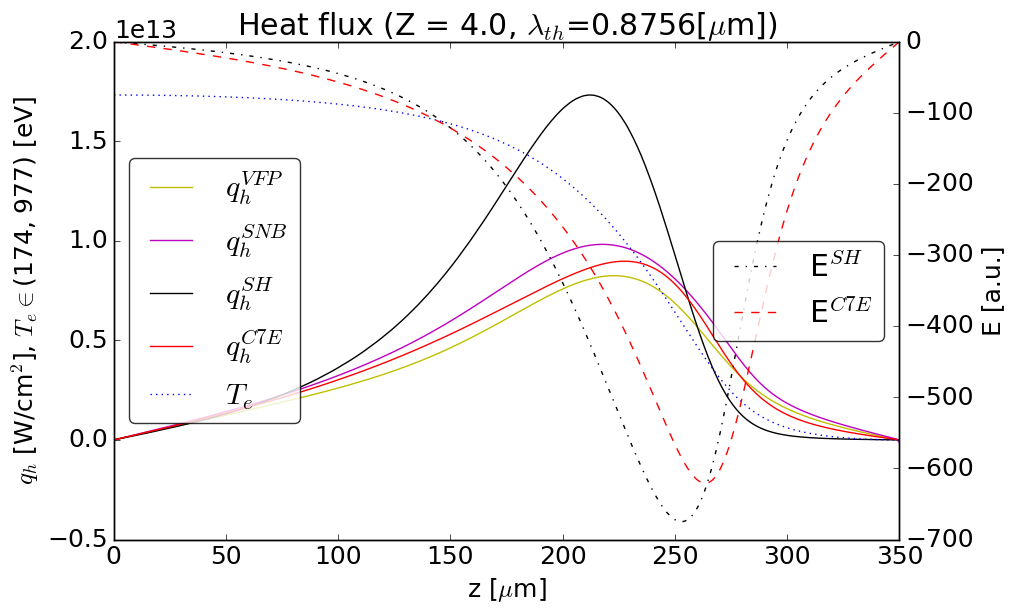
\includegraphics[width=1.0\textwidth]{../VFPdata/C7_heatflux_12ps.png} \\ 
      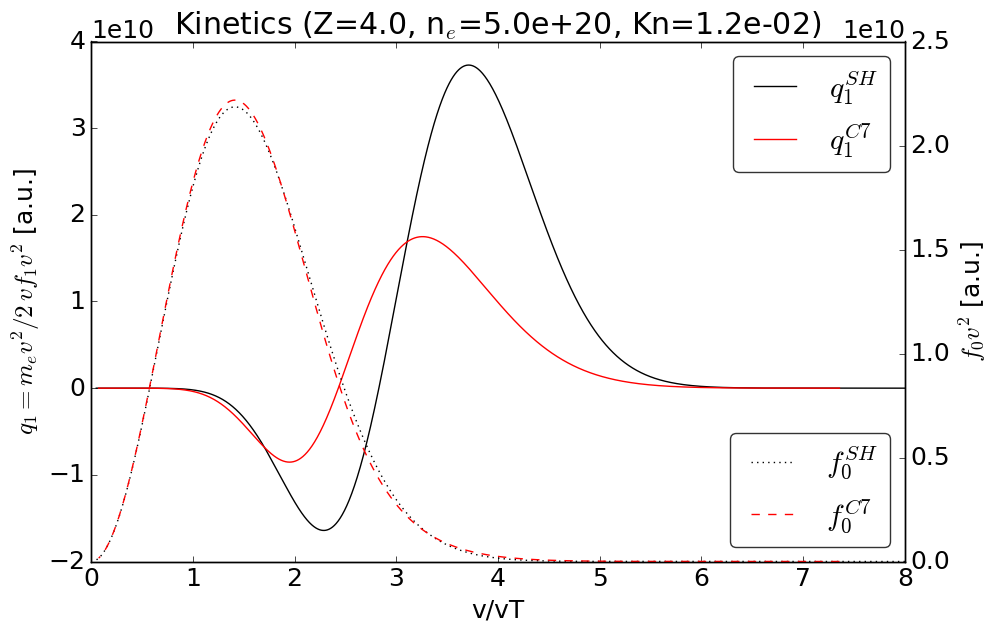
\includegraphics[width=1.0\textwidth]{../VFPdata/C7_kinetics_12ps.png}
    \end{tabular}
  \caption{
  Philippe's preferred test $\Zbar = 4$ at 12 ps.  
  }
  \end{center}
  \label{fig:Philippe_VFP_12ps}
\end{figure}

\begin{figure}[tbh]
  \begin{center}
    \begin{tabular}{c}
      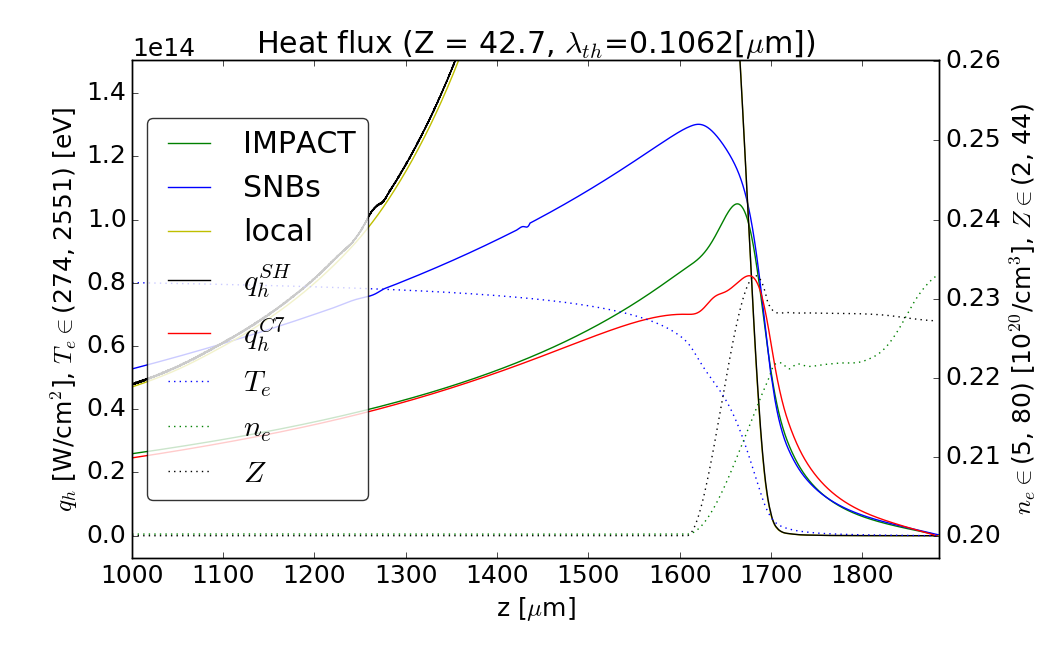
\includegraphics[width=1.0\textwidth]{../VFPdata/GD_Hohlraum/fluxes_10ps.png} \\
      %\includegraphics[width=1.0\textwidth]{../VFPdata/GD_Hohlraum/diffusion_fluxes_10ps.png} 
      %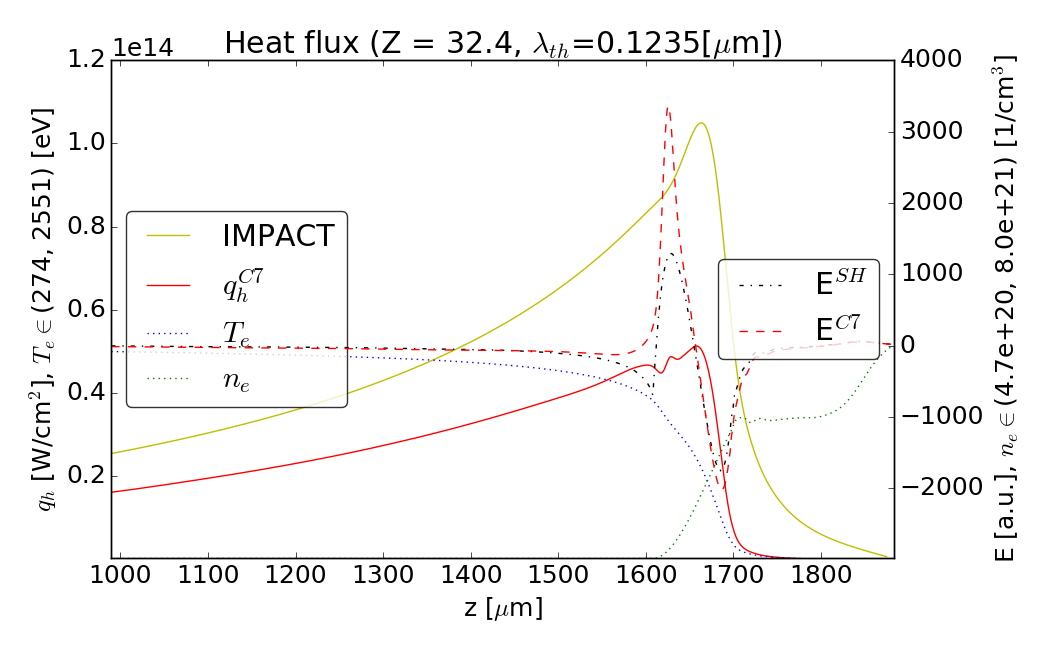
\includegraphics[width=1.0\textwidth]{../VFPdata/GD_Hohlraum/fluxes_Efield_10ps.png} \\ 
      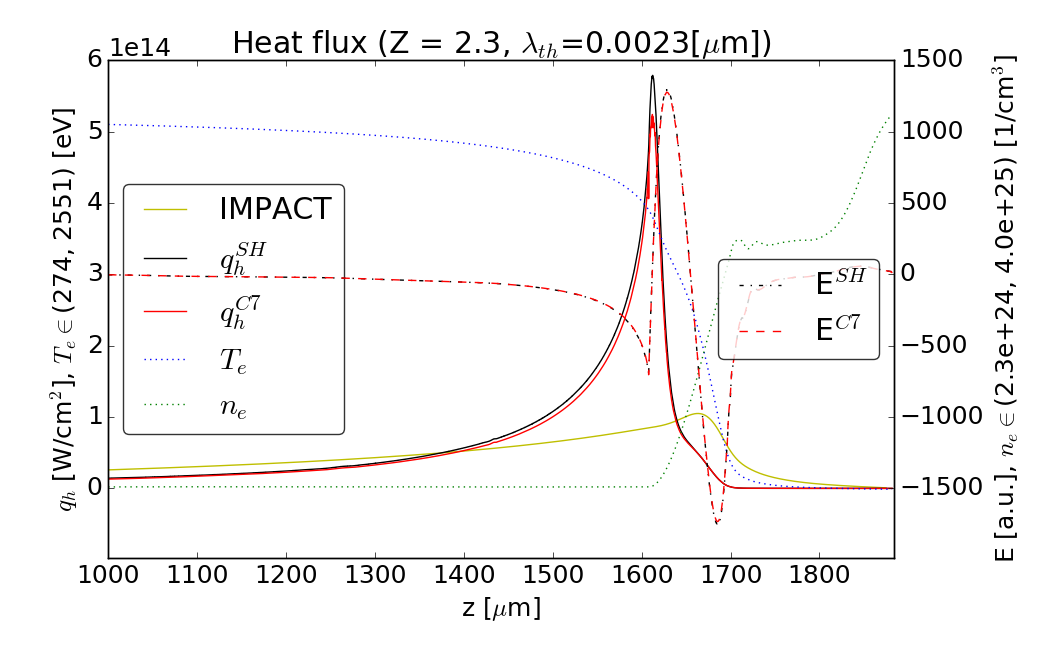
\includegraphics[width=1.0\textwidth]{../VFPdata/GD_Hohlraum/diffusion_fluxes_Efield_10ps.png} 
    \end{tabular}
  \caption{
  }
  \end{center}
  \label{fig:Gd_VFP_10ps_heatflux}
\end{figure}

\begin{figure}[tbh]
  \begin{center}
    \begin{tabular}{c}
       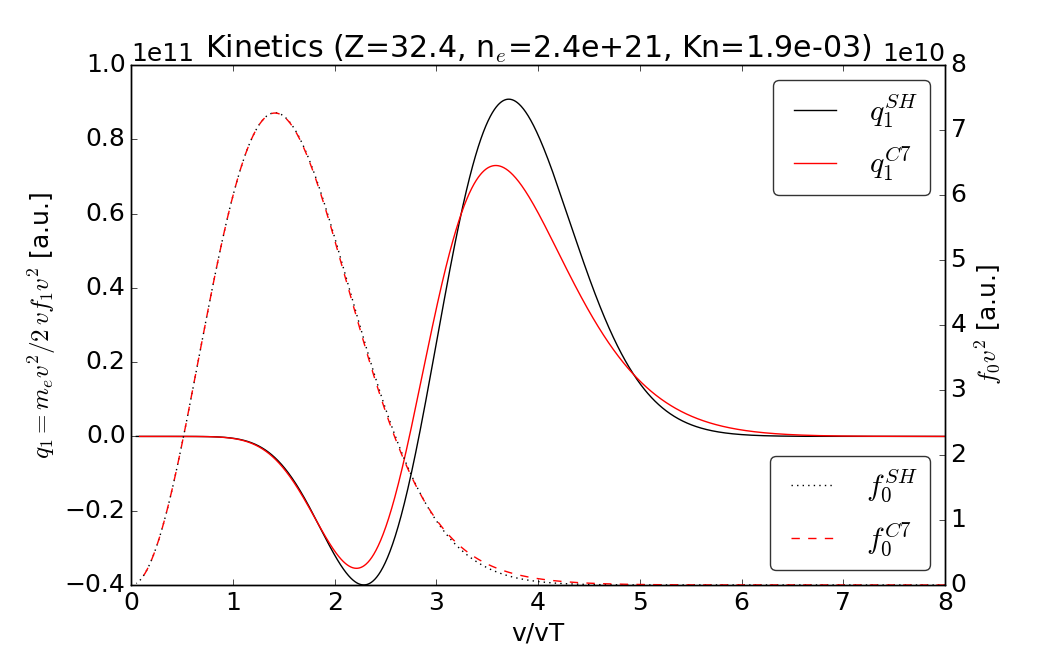
\includegraphics[width=1.0\textwidth]{../VFPdata/GD_Hohlraum/kinetics_10ps_xpointmax.png} \\ 
      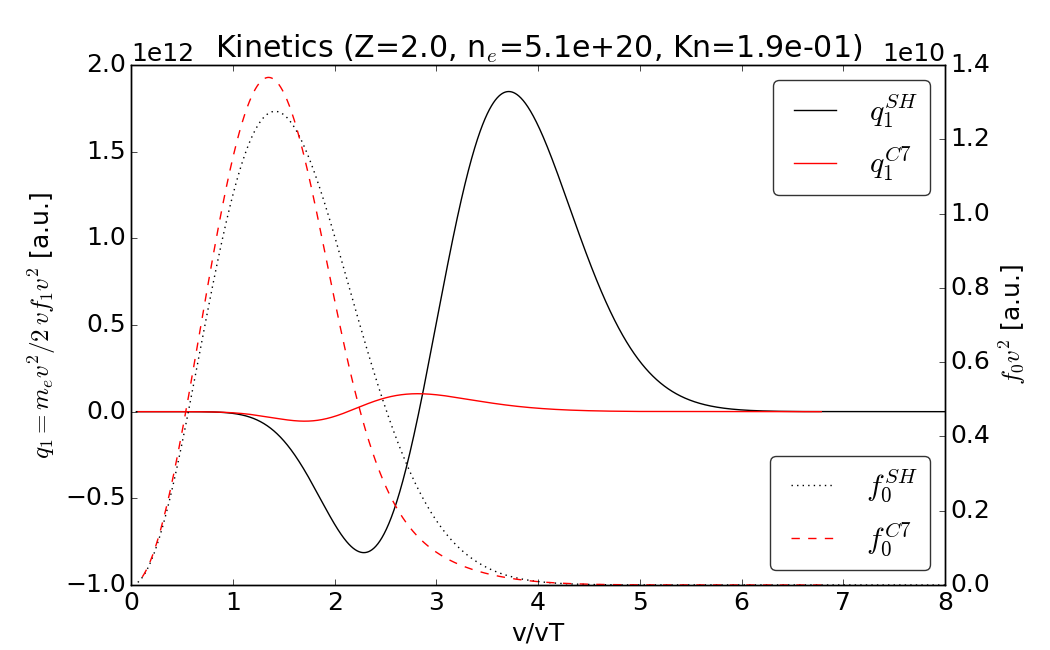
\includegraphics[width=1.0\textwidth]{../VFPdata/GD_Hohlraum/kinetics_10ps_xpoint_1605microns.png}
    \end{tabular}
  \caption{
  Kinetics profiles for max(flux) point and 1605 microns point for the case of 10ps VFP temperature profile, ne and Z Hydra profiles. 
  }
  \end{center}
  \label{fig:Gd_VFP_10ps_kinetics}
\end{figure}

\begin{figure}[tbh]
  \begin{center}
    \begin{tabular}{c}
      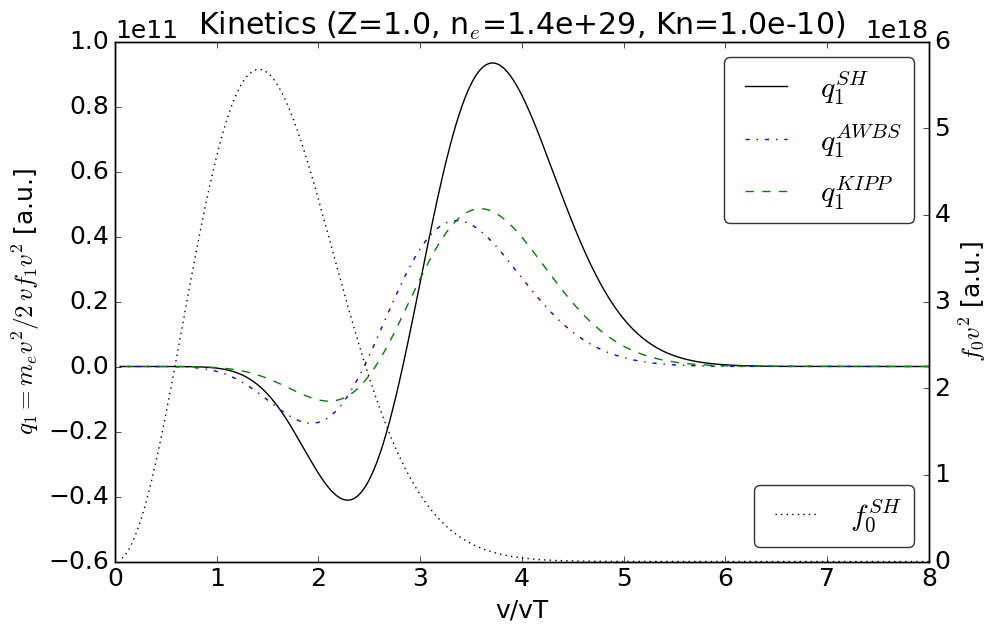
\includegraphics[width=1.0\textwidth]{../VFPdata/KIPP_q_kinetics.png} \\
      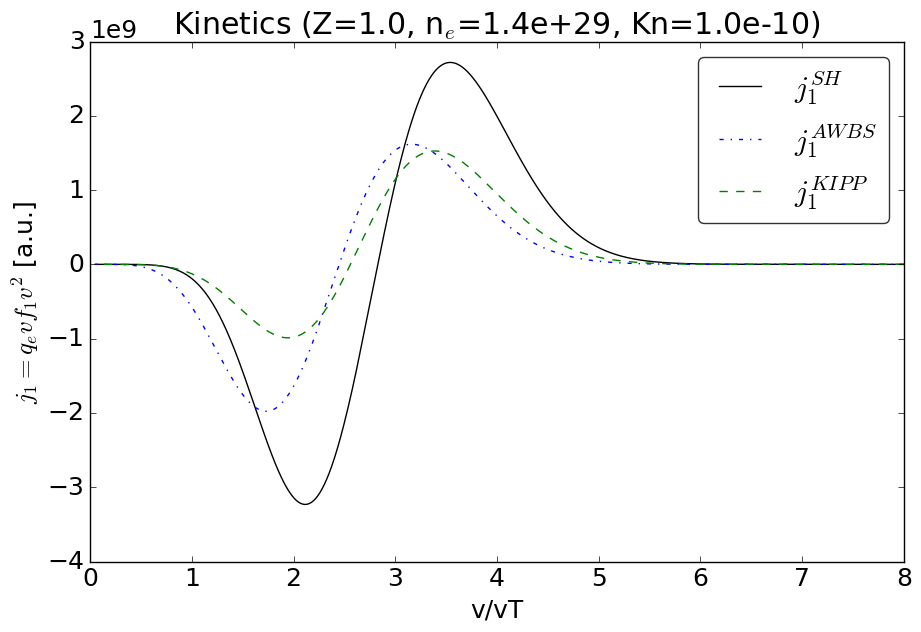
\includegraphics[width=1.0\textwidth]{../VFPdata/KIPP_j_kinetics.png}
    \end{tabular}
  \caption{KIPP (by Johnathan) vs AWBS using 
  $\mfpei^* = \frac{\Zbar + 0.24}{\Zbar + 4.2}\mfpei, \Zbar=1, 
  \vth = \sqrt{\frac{\kB T_e}{\me}}$ 
  $f_1^{SH} = -\mfpei^*(v) \left(\frac{v^2}{2 \vth^2} - 4\right) 
  \frac{\vn\cdot\nabla T_e}{T_e} \fM,\quad 
  f_1^{KIPP} = -\mfpei^*(v) \left(\frac{3}{16}\frac{v^2}{\vth^2} - 1 
  - \frac{3}{2}\frac{\vth^2}{v^2} \right) 
  \frac{\vn\cdot\nabla T_e}{T_e} \fM$.
  }
  \end{center}
  \label{fig:}
\end{figure}

\begin{figure}[tbh]
  \begin{center}
    \begin{tabular}{c}
      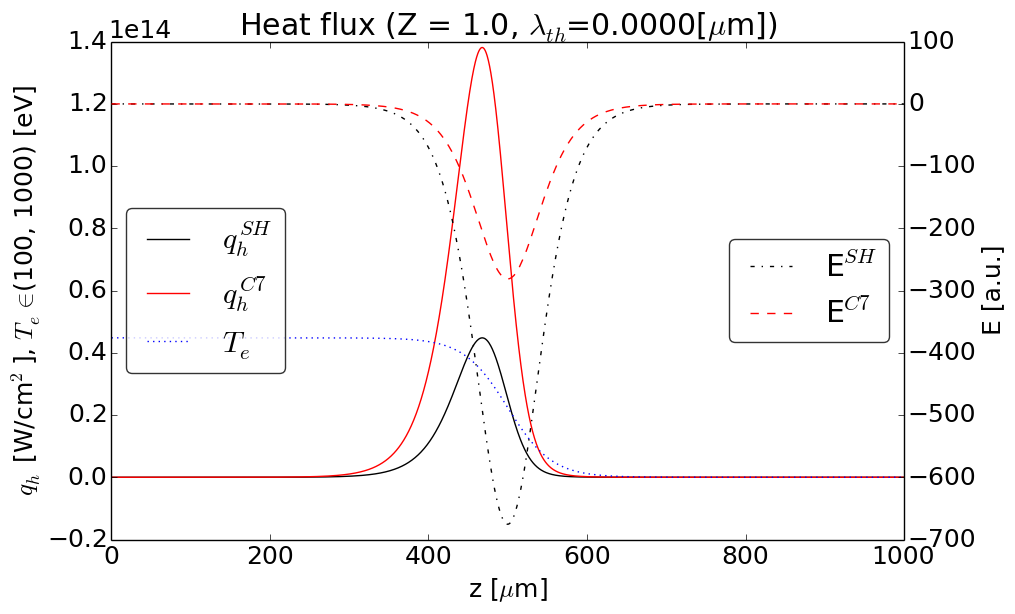
\includegraphics[width=1.0\textwidth]{../results/fe_analysis/figs/P5_diffusive_heatflux_Z1_decelerating_Ezerothiter.png} \\
      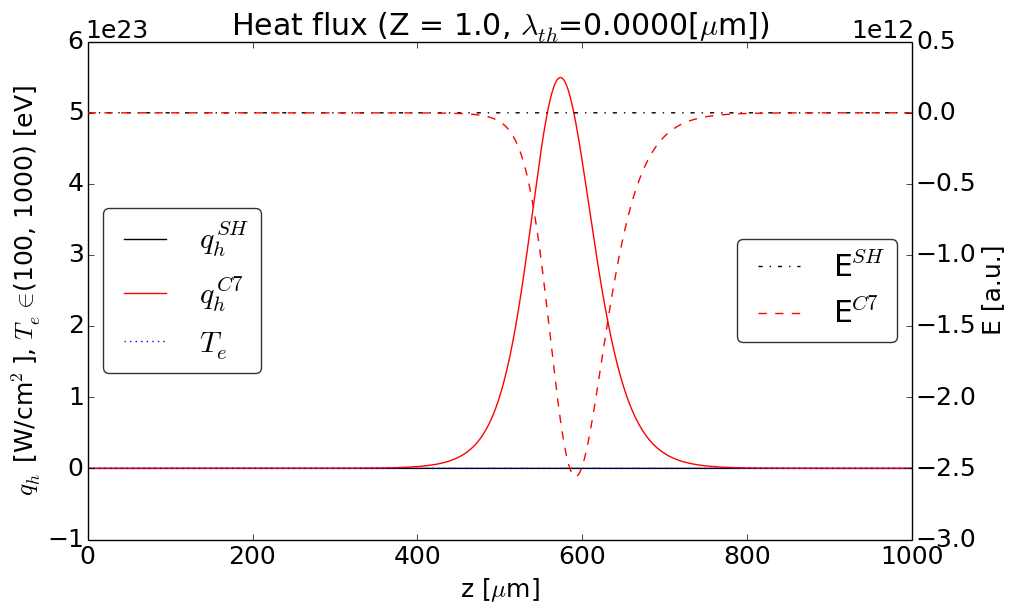
\includegraphics[width=1.0\textwidth]{../results/fe_analysis/figs/P5_diffusive_heatflux_Z1_accelerating_Ezerothiter.png}
    \end{tabular}
  \caption{
  Decelerating (top) vs. accelerating (bottom) computations. 
  Zeroth E field iteration, i.e.
  no E field effect, of the diffusion regime conditions.
  }
  \end{center}
  \label{fig:}
\end{figure}

\clearpage

%\begin{figure}[tbh]
%  \begin{center}
%    \begin{tabular}{c}
%      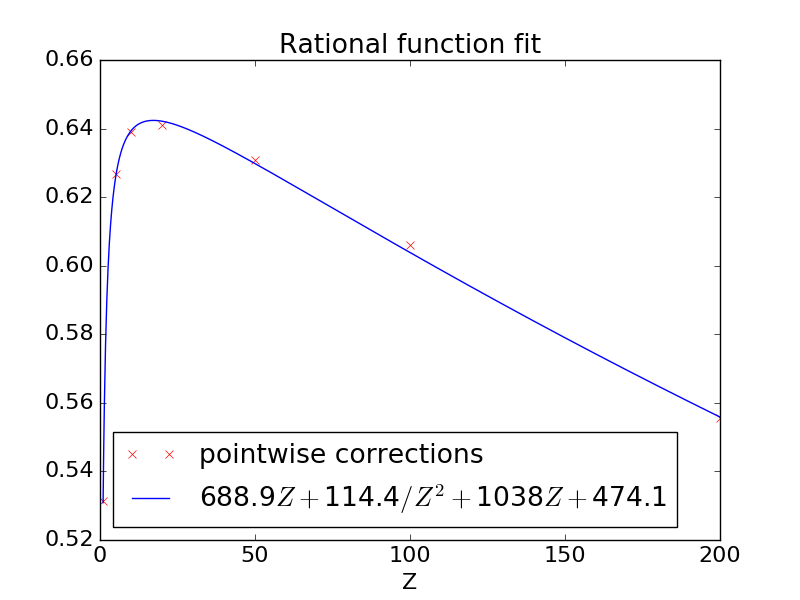
\includegraphics[width=0.55\textwidth]{../results/fe_analysis/figs/AWBScorrection_fit.png} 
%    \end{tabular}
%  \caption{
%  Analytic fit to the~Z correction 
%  ($\nue^* = \frac{688.9 \Zbar + 114.4}{\Zbar^2 + 
%  1038 \Zbar + 474.1} \nue$, where $\nue = \nuei / \Zbar$) 
%  of the~diffusion asymptotic of AWBS with respect to SH.
%  }
%  \end{center}
%  \label{fig:}
%\end{figure}

%% The Appendices part is started with the command \appendix;
%% appendix sections are then done as normal sections
%% \appendix

%% \section{}
%% \label{}

%% References
%%
%% Following citation commands can be used in the body text:
%% Usage of \cite is as follows:
%%   \cite{key}         ==>>  [#]
%%   \cite[chap. 2]{key} ==>> [#, chap. 2]
%%

%% References with bibTeX database:

\bibliographystyle{elsarticle-num}
\bibliography{NTH}

%% Authors are advised to submit their bibtex database files. They are
%% requested to list a bibtex style file in the manuscript if they do
%% not want to use elsarticle-num.bst.

%% References without bibTeX database:

% \begin{thebibliography}{00}

%% \bibitem must have the following form:
%%   \bibitem{key}...
%%

% \bibitem{}

% \end{thebibliography}


\end{document}

%%
%% End of file 
